\chapter{Experiments in live introspection}
\label{ch:experiments}

This chapter serves the purpose of showcasing the library and validating its
usefulness for actual deep learning research. While the ultimate goal is to have
a set of well-researched metrics in place which can be used live during
training, the way to acquire these metrics requires extensive analysis from many
experiments. Therefore, the goal of this work is to research candidate metrics,
not actually use them to improve any particular model's performance on any
specific problem. This entails that the library is used primarily for easily
gathering all the data from the necessary experiments and computing candidate
metrics, and not for supervising the actual training.

The chapter is divided between a reproduction part (see
\cref{sec:adam}) and an original research part (see
\cref{sec:detecting_learning_rate_proprocess} and
\cref{sec:detecting_layer_saturation}). In the former, experiments conducted
for a popular variant of stochastic gradient descent (hence referred to as SGD
) are reproduced and extended with
the help of the library. The goal is to fact-check claims made by the authors
and validate said claims on more scenarios than are shown in the
publication. This will serve to show how \texttt{ikkuna} could have been
employed for this type of work. The second part will be concerned with employing
the library to investigate hypotheses for diagnosing roadblocks in the training
process. Recall from \cref{sec:motivation} the multitude of hyperparameters
for a deep learning model and training regimen. In this work, we will concern
ourselves with the question of figuring out a good learning rate and when to
stop training layers to reduce computation time.

This thesis is not concerned with advancing the state of the art in
classification. Instead, toy problems are developed in order to prove or
disprove that the proposed metrics have the potential to be useful in guiding
the training. A more thorough evaluation of the results on realistic
architectures and problem sizes would require significantly more time and
computational resources and is left for future work.

\section{Experimental Methodology}%
\label{sec:experimental_methodology}

For all experiments, \texttt{ikkuna} is used for recording various metrics
during training without having to adapt to any specific model. Experiments are
run on a Google Cloud virtual instance with between $4$ and $8$ Intel Xeon CPUs
and $1$ to $2$  Nvidia Tesla K80 graphics cards with $11$ GB of video memory. The
information captured by \texttt{ikkuna} during training is logged to a MongoDB
schemaless database with the help of the \texttt{sacred} library. The data can
then be analysed off-line with MongoDB's Python interface. Plots are created
with \texttt{matplotlib}. % and \texttt{seaborn}.

\section{Validating Optimiser Research}%
\label{sec:adam}

In this section, we want to highlight the \texttt{ikkuna}'s usefulness in
scientific research by conducting experiments in the context of
\citep{kingma2014adam} and investigating in how far the claims made therein hold
true on a range of problems. The work investigates the Adam optimisation
algorithm on several machine learning problems, notably learning a convolutional
network on the CIFAR10 dataset.

\subsection{The Adam update rule}%
\label{sub:the_adam_update_rule}

While standard SGD only makes use of the gradients in the current time step to
compute a parameter update, Adam keeps an exponential moving average of the
gradient ($m_t$) and its square ($v_t$), supposedly as an estimate for the mean
and variance of the gradient around the current point in parameter space. This
estimate is computed for each parameter, meaning Adam incurs a memory overhead
of $\mathcal{O}(d)$ where $d$ is the number of model parameters. Since the
estimates are initialised with zero, a bias correction (denoted by
$\widehat{\cdot}$~) is applied.

The parameter updates are computed as
\begin{align}
    \theta_t \leftarrow \theta_{t-1}  - \eta \frac{\widehat{m}_t}{\sqrt{\widehat{v}_t} +
    \epsilon}
    \label{eq:adam}
\end{align}
\citeauthor{kingma2014adam} justify the rule like this:
\begin{quote}
    With a smaller SNR [quotient of mean and square root of variance] the
    effective stepsize $\Delta_t$ will be closer to zero. This is a desirable
    property, since a smaller SNR means that there is greater uncertainty about
    whether the direction of $m_t$ corresponds to the direction of the true
    gradient. For example, the SNR value typically becomes closer to $0$ towards
    an optimum, leading to smaller effective steps in parameter space: a form of
    automatic annealing.
\end{quote}

Intuitively, the magnitudes of the update to a parameter will scale linearly
with the manitude of the running gradient mean (which is effectively a form of
momentum), but normalised with the magnitude of the running gradient variance so
that the update is smaller when the gradient is very noisy and larger when there
is more certainty of the direction of the true gradient.

\subsubsection{The Role of \texttt{ikkuna}}%
\label{sub:use_of_ikkuna_for_optimiser_research}

We use the \texttt{ikkuna} library to compute and record various metrics during
reproduction and extension of \citeauthor{kingma2014adam}'s experiments. This
section showcases how little code is required to implement a recording setup
portable to any neural network model. A subscriber is employed to record
\begin{enumerate}
    \item The biased first moment estimate (exponential running gradient)
    \item The biased second moment estimate (exponential running squared
        gradient)
    \item The bias-corrected first moment estimate
    \item The bias-corrected second moment estimate
    \item The effective learning rate
\end{enumerate}

For all metrics, mean, variance, median, and norm are logged in some interval,
as computing the median incurs $\mathcal{O}(n\log n)$ runtime cost for each
layer. Since Adam doesn't directly use the current gradients for its parameter
updates, we need to extract the effective learning rate used for a layer
somehow. Since we have access to the gradient $\nabla_t(L)$ and the update
$\Delta_t$ in each train step, we can divide the two to obtain
$\frac{\Delta_t}{\nabla_t(L)}=\eta$ which is the learning rate we would need to
use in a vanilla SGD step with the current gradients. However, gradients can be
zero at any time, and the corresponding update may not be, since Adam uses
gradients from the previous steps as well. We thus simply ignore invalid values
through division by zero in computing the metrics. In the pathological case
where this leads to an empty tensor, we plot NaN (leading to an omission of the
value), since we would otherwise have to work around metric logs with different
step vectors.

The subscriber used for recording all the information is displayed in
\cref{lst:running_moments_sub}. A second subscriber is used to log all the
computed metrics to a MongoDB database via the \texttt{sacred} library. While
the cleaner approach here would be to implement a \texttt{SacredBackend} to log
the metrics automatically, this would require some thought about the differing
capabilities of different backends. For instance, there is no native form of
histogram storage in \texttt{sacred}, while it is easy to provide through
TensorBoard or Matplotlib. Therefore, this backend is left for future work and a
Subscriber ist used instead for this limited set of experiments.

\begin{lstlisting}[label={lst:running_moments_sub},
caption={Subscriber to record Adam terms}]
class BiasCorrectedMomentsSubscriber(PlotSubscriber):

  def __init__(self, lr, beta1, beta2, eps, message_bus=get_default_bus(), tag=None, subsample=40, ylims=None, backend='tb'):

    title        = 'gradient_moments'
    ylabel       = 'Gradient Moments'
    xlabel       = 'Train step'
    subscription = Subscription(self, ['weight_gradients'], tag, subsample)
    super().__init__([subscription], message_bus,
                     {'title': title,
                      'ylabel': ylabel,
                      'ylims': ylims,
                      'xlabel': xlabel},
                     backend=backend)

    # all parameters to Adam
    self._lr    = lr
    self._beta1 = beta1
    self._beta2 = beta2
    self._eps   = eps

    # records of the running moment estimates
    self._means = dict()
    self._vars  = dict()

    # here we set up all the metrics to be published
    for pub_name in {
      'biased_grad_mean_estimate_mean',
      'biased_grad_mean_estimate_median',
      'biased_grad_mean_estimate_var',
      'biased_grad_var_estimate_mean',
      'biased_grad_var_estimate_median',
      'biased_grad_var_estimate_var',
      'biased_grad_mean_estimate_norm',
      'biased_grad_var_estimate_norm',
      'grad_mean_estimate_mean',
      'grad_mean_estimate_median',
      'grad_mean_estimate_var',
      'grad_var_estimate_mean',
      'grad_var_estimate_median',
      'grad_var_estimate_var',
      'grad_mean_estimate_norm',
      'grad_var_estimate_norm',
      'effective_lr_mean',
      'effective_lr_median',
      'effective_lr_var',
      'effective_lr_norm',
    }:
      self._add_publication(pub_name, type='DATA')

  def compute(self, message):

    named_module = message.key

    grad         = message.data
    t            = message.global_step + 1

    # init moving moments if not present
    if named_module not in self._means:
      self._means[named_module] = torch.zeros_like(grad)
      if named_module not in self._vars:
        self._vars[named_module] = torch.zeros_like(grad)

    exp_avg, exp_avg_sq = self._means[named_module], self._vars[named_module]
    beta1, beta2        = self._beta1, self._beta2

    exp_avg.mul_(beta1).add_(1 - beta1, grad)
    exp_avg_sq.mul_(beta2).addcmul_(1 - beta2, grad, grad)

    # we use the more efficient ordering of computation from Kingma et al. (p.
    # 2) used in PyTorch's implementation
    bias_correction1    = 1 - beta1 ** t
    bias_correction2    = 1 - beta2 ** t
    unbiased_exp_avg    = exp_avg / bias_correction1
    unbiased_exp_avg_sq = exp_avg_sq / bias_correction2
    step_size           = self._lr * math.sqrt(bias_correction2) / bias_correction1
    denom               = exp_avg_sq.sqrt().add_(self._eps)

    # here we basically revert the entire thing to get the effective learning
    # rate
    update              = step_size * exp_avg / denom
    update.div_(grad)
    nan_tensor          = torch.isnan(update)
    inf_tensor          = torch.isinf(update)
    effective_lr        = update[(1 - nan_tensor) & (1 - inf_tensor)]

    # it's possible to end up with no valid values -> log 0 so plotting doesn't
    # crash (nan may also have worked)
    if grad.sum() == torch.tensor(0.0).cuda():
      # this would mean all entries are nan or inf because the current gradient was
      # zero
      effective_lr = torch.tensor(0.0).cuda()

    # instead of repeating the call to publish_module_message for each topic, look at
    # all topic names and infer the local variable from the topic name
    for topic in self.publications['DATA']:

      if topic.startswith('biased_grad_mean'):
        data = exp_avg
      elif topic.startswith('biased_grad_var'):
        data = exp_avg_sq
      elif topic.startswith('grad_mean'):
        data = unbiased_exp_avg
      elif topic.startswith('grad_var'):
        data = unbiased_exp_avg_sq
      elif topic.startswith('effective_lr'):
        data = effective_lr
      else:
        raise ValueError(f'Unexpected topic "{topic}"')

      if topic.endswith('norm'):
        data = data.norm()
      elif topic.endswith('mean'):
        data = data.mean()
      elif topic.endswith('median'):
        data = data.median()
      elif topic.endswith('var'):
        data = data.var()
      else:
        raise ValueError(f'Unexpected topic "{topic}"')

      self.message_bus.publish_module_message(message.global_step,
                                              message.train_step,
                                              message.epoch, topic,
                                              message.key, data)
\end{lstlisting}

The subscriber for logging the metrics is trivial:
\begin{lstlisting}
class SacredLoggingSubscriber(Subscriber):
  '''Subscriber which logs its subscribed values with sacred's metrics API'''

  def __init__(self, experiment, kinds):
    self._experiment = experiment
    subscription     = Subscription(self, kinds)
    super().__init__([subscription], get_default_bus())

  def compute(self, message):
    if message.key != 'META':
      name = f'{message.kind}.{message.key.name}'
    else:
      name = message.kind
  self._experiment.log_scalar(name, float(message.data), message.global_step)
\end{lstlisting}


\subsection{Experiments}%
\label{sub:experiments}

The experiments conducted here all use the CIFAR10 dataset learned by a range of
models (among them the one presumably used in \citet{kingma2014adam}). The
dataset is whitened\footnote{Since I did not manage to implement the
preprocessing correctly, the dataset used here is from
\url{https://github.com/szagoruyko/wide-residual-networks}}.

The convolutional network (\cref{fig:adammodel}) used by the authors is not unambigously described in
the publication, so it cannot be guaranteed that the reproduction is accurate.
The experiments here also omit the dropout applied to the input layer (it is
unclear whether \citeauthor{kingma2014adam} refer to the float-converted input
data itself, which would generally be called the input layer to or the initial
layer of convolutions) because the network did not learn anything in that case
and the dropout probability is not specified. We further perform the experiments
on a fully-connected network without convolutional layers (see
\cref{fig:fully-connected}) as well as the previously introduced VGG
architecture (\cref{fig:vgg16}).

\begin{figure}
    \centering
    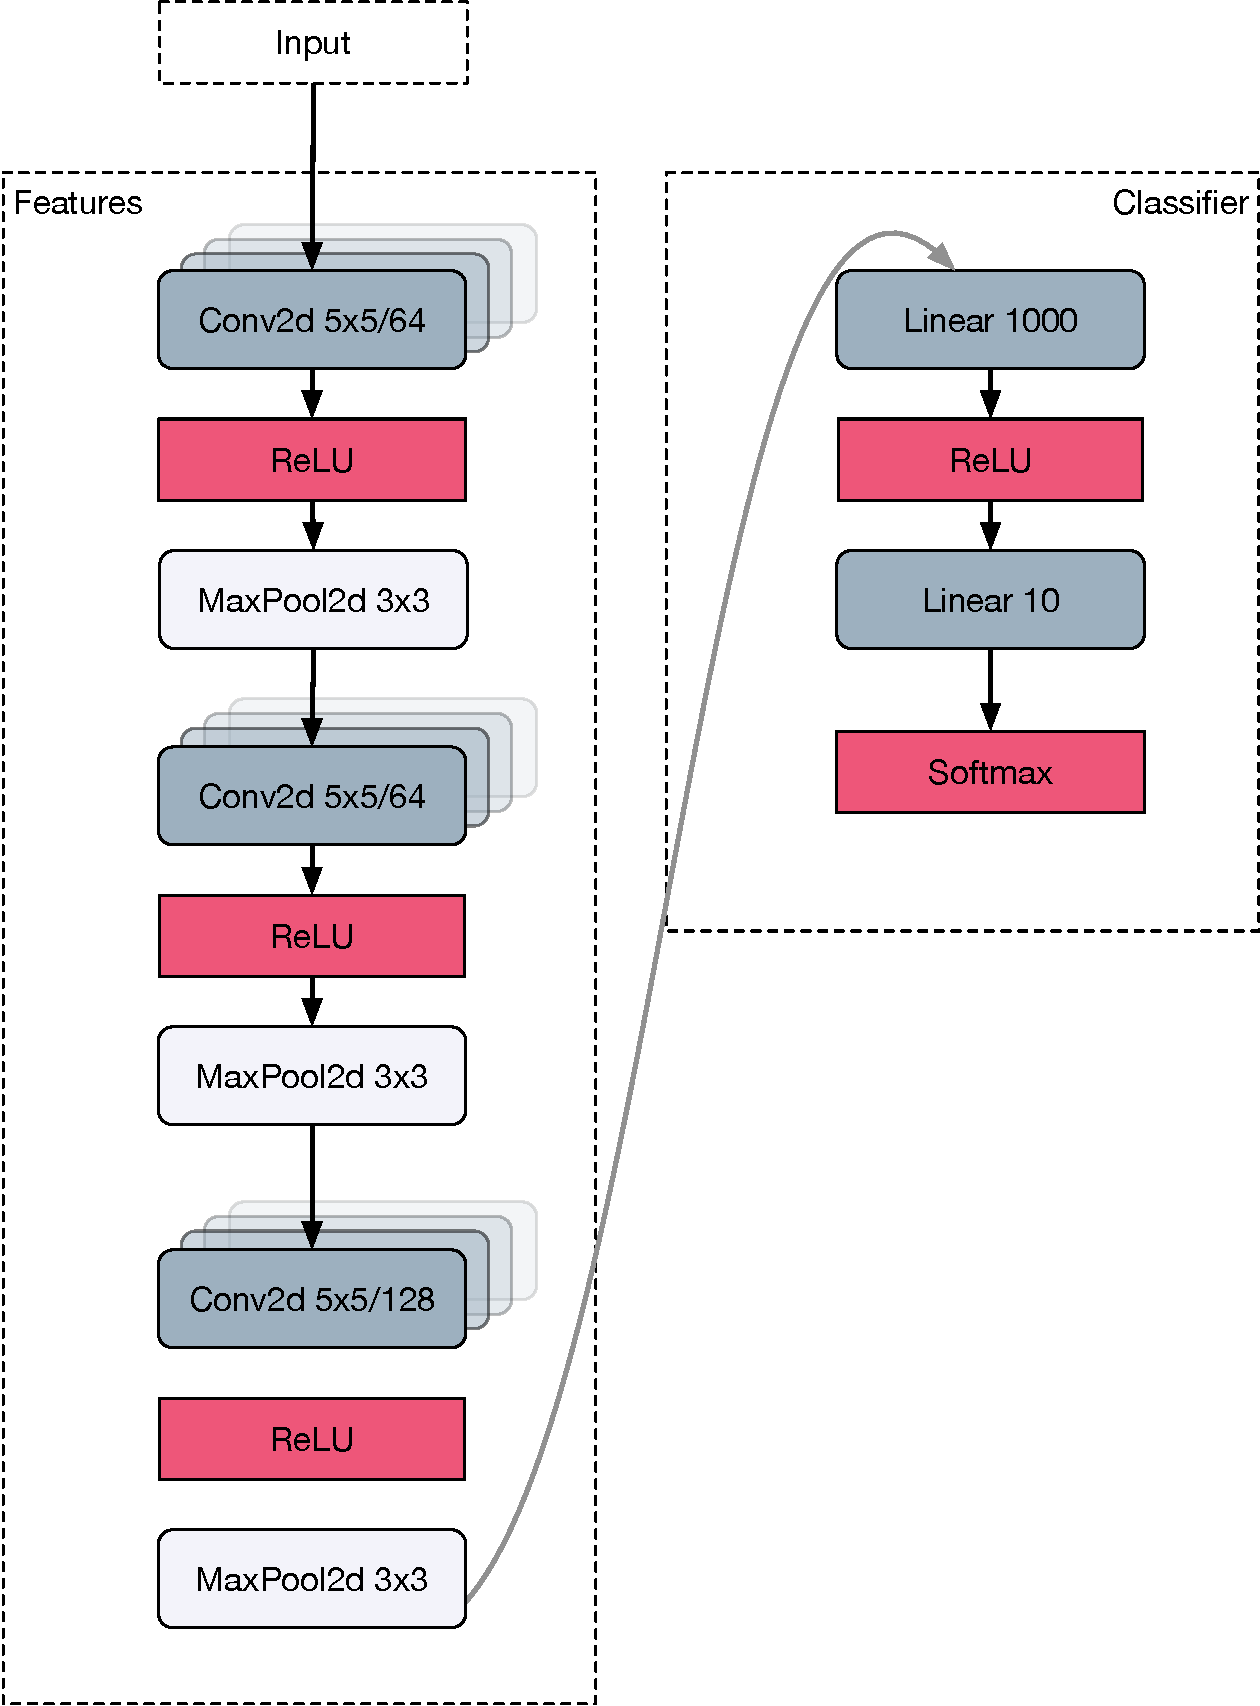
\includegraphics[width=.8\linewidth]{gfx/diagrams/neural_network/adammodel.pdf}
    \caption{Probable Adam model architecture}
    \label{fig:adammodel}
\end{figure}

\begin{figure}
    \centering
    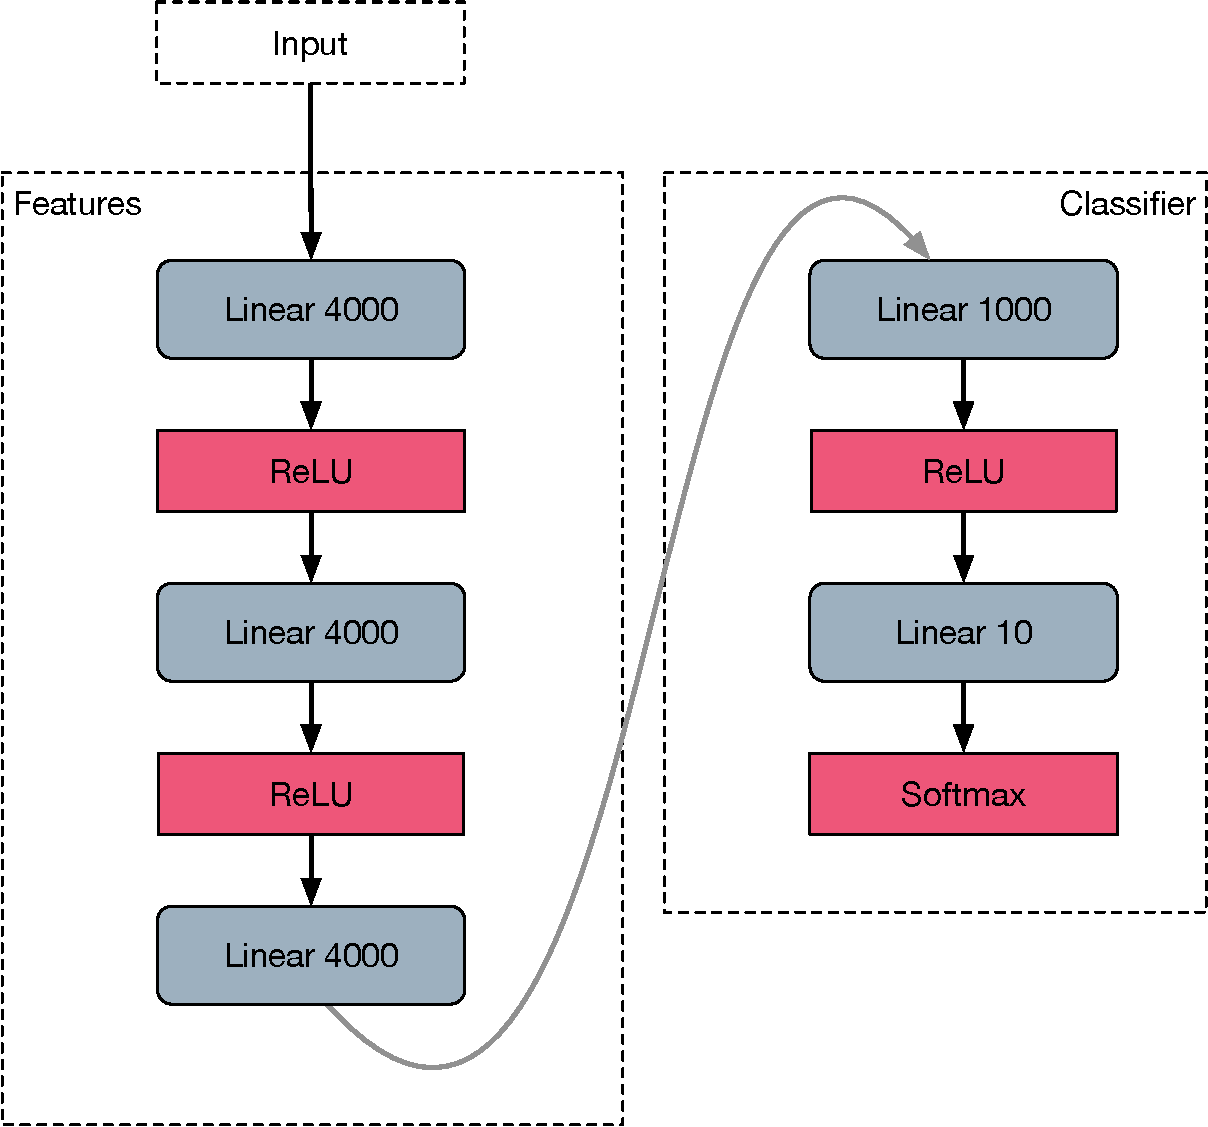
\includegraphics[width=.8\linewidth]{gfx/diagrams/neural_network/fullyconnected.pdf}
    \caption{Purely dense model}
    \label{fig:fully-connected}
\end{figure}

We want to employ \texttt{ikkuna} to monitor the quantities in Adam's update
rule on varous architectures. This will allow us to investigate whether there is
a qualitative difference in how Adam operates on different architectures, as
well as shed light on its behaviour in cases where it fails to optimise the
network. We also track the same quantites with vanilla SGD for comparison.
Additionally, the authors make claims in the publication without accompanying
evidence, notably

\begin{itemize}
    \item \label{itm:adam-claim-1} Convolutional layers should be assigned a smaller learning rate than
        linear ones and that---presumably---Adam does this automatically.
    \item
        That the update for the experiment with the convolutional network is
        dominated by the mean estimate and $\epsilon$ while the gradient
        variance estimate vanishes to zero after a few epochs.
\end{itemize}
Whether these assertions hold true will also be investigated.

It should be noted that the quantities used in \cref{eq:adam} are tensor-valued,
i.e. the estimates of the gradient moments are computed for each parameter.
Since visualising all parameters individually is not only computationally
infeasible, but also useless, some level of granularity with an appropriate
summary measure needs to be defined. The next level of organisation above
individual layer weights are the weight tensors themselves. Since layers are the
basic building blocks, it makes sense to investigate Adam's behaviour on the
level of individual layers. The question of how to summarise e.g. the gradient
mean estimate for an entire layer remains. Candidates are
\begin{enumerate}
    \item the average over all units
    \item the norm of the estimate
    \item the median over all units
\end{enumerate}
The first option suffers from the fact that the gradient distribution is
centered around zero, so the values for most layers empirically average out.
The norm of the estimate on the other hand gives a sense of the total magnitude and thus the total
change to a layer. The last option is computationally more demanding, but
prevents the problem of outliers, while also suffering from the fact that the
gradient distribution is mostly centered around zero. We will therefore plot the
norm of the first moment estimate since we are mostly interested in how much
total contribution the term has for in the update. For the second moment, we
plot the median, since all values are larger than $1$ and thus cannot average
out. Norm, mean and median will exhibit similar qualitative behaviour for this
term anyway, so the choice is less critical. For plotting effective learning
rates, we once again report the median, as they vary a lot within a layer and we
would like to have some form of average so it fits with our concept of a
actual learning rate.

\subsubsection{Reproducing the Convnet experiment}

As a start, we check whether we can successfully recreate the experiment from
\citep{kingma2014adam} with the convolutional architecture. On p. 7 they show
the performance of the network over the first three epochs and the entire
training time. Our reproduction with the exact same parameters  is shown in
\cref{fig:adam-repro}.

\begin{figure}
    \begin{subfigure}{\textwidth}
        \centering
        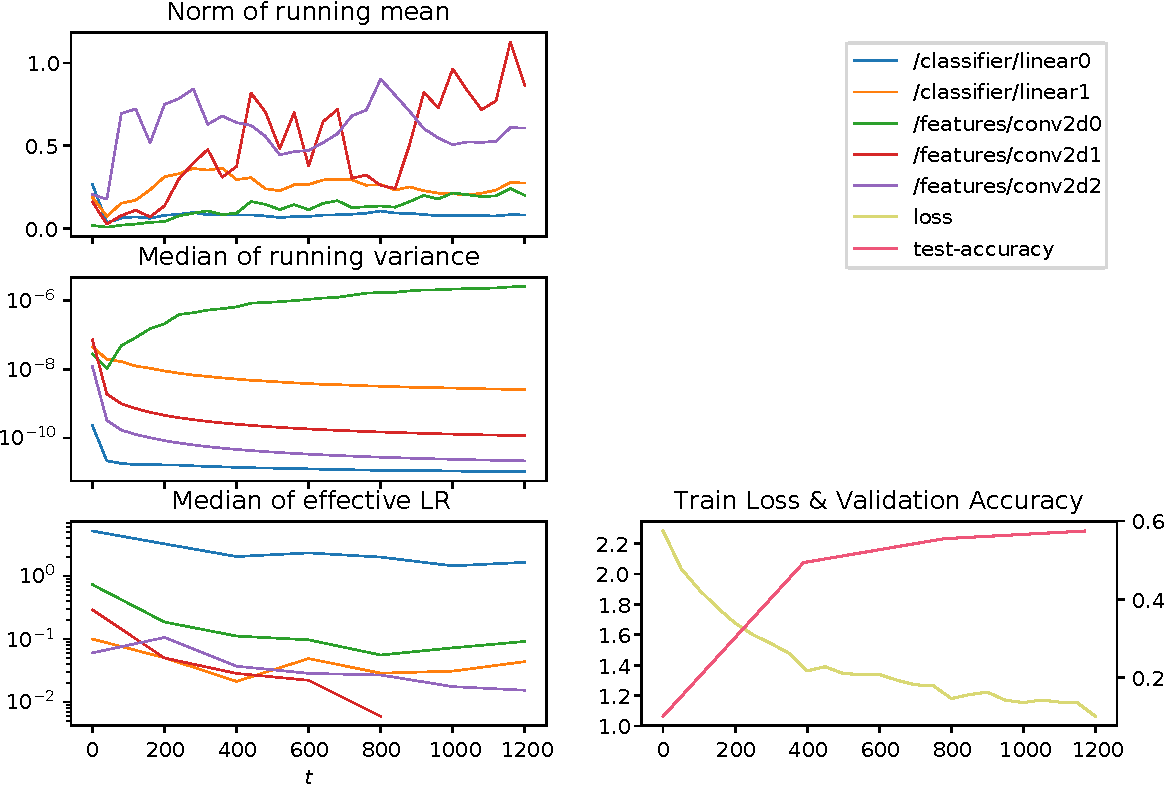
\includegraphics[width=\linewidth]{gfx/diagrams/experiments/adam/adammodel_adam_0001_0_1200.pdf}
        \caption{Adam convnet with learning rate $0.001$, first three epochs}
        \label{fig:adam-repro-1}
    \end{subfigure}

    \begin{subfigure}{\textwidth}
        \centering
        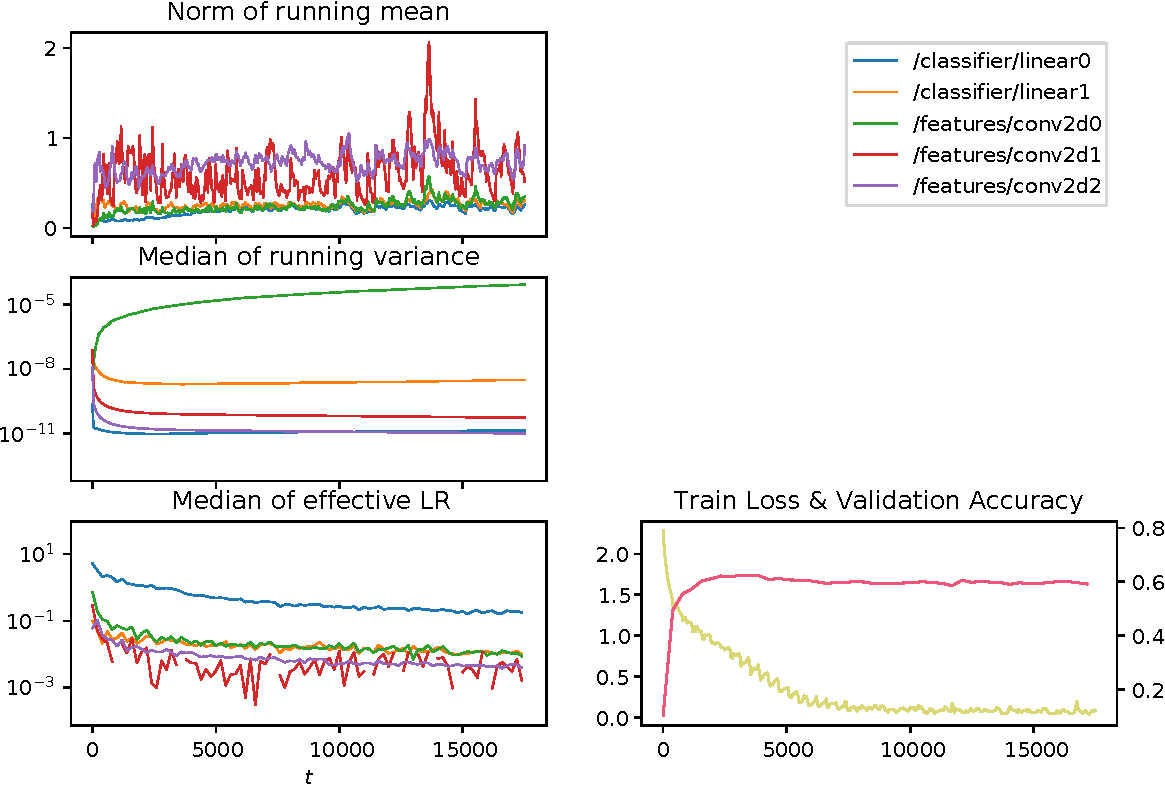
\includegraphics[width=\linewidth]{gfx/diagrams/experiments/adam/adammodel_adam_0001_0_-1.pdf}
        \caption{Adam convnet with learning rate $0.001$, entire training}
        \label{fig:adam-repro-2}
    \end{subfigure}
    \label{fig:adam-repro}
\end{figure}

\citeauthor{kingma2014adam} report a decrease of the training cost from $\sim
2.2$ down to around $0.4$ over the course of the first three epochs. In our
reproduction (\cref{fig:adam-repro-1}), the loss does not decrease that rapidly,
but the trajectory is broadly similar, also when considering the entire training
(\cref{fig:adam-repro-2}). Nevertheless, the original setup achieves training
loss of less than $0.001$ while our experiment does not improve beyond $0.05$.
In \citeauthor{kingma2014adam}'s experiment, the training loss almost saturates
after about 20 epochs, the same holds for our reproduction. However, the
original result shows the network gradually learning the entire time whereas
performance basically stalls in our reproduction after 20 epochs. We can thus
not completely reproduces the original experiment.  Possible reasons are an
incorrectly specified architecture, a different loss function\footnote{This is
    very unlikely, as the categorical crossentropy is almost always used for
classification tasks, and also the absolute values are rather similar.}, or
details of the training procedure which \citeauthor{kingma2014adam} do not
mention.

We can also see that in our experiment, the claim that
\begin{quote}
 the second moment estimate $v_t$ vanishes to zeros after a few epochs and is
 dominated by the $\epsilon$ in [the update rule]
\end{quote}
does not hold true. Just as in the paper, we set $\epsilon = 10^{-8}$, but the
median second moment estimate only vanishes for some layers and increases even
for the first convolutional layer. Saying that the update is ``dominated'' by
$\epsilon$ may therefore be inaccurate, at least we cannot show this to be the
case. It is unclear how \citeauthor{kingma2014adam} evaluate the tensor-valued
second moment estimate to arrive at this conclusion.

We will now turn to a qualitative and quantitative evaluation of how Adam
performs on fully-connected and convolutional architectures and whether it
actually tunes the learning rate like \citet{kingma2014adam} suggest.

\subsubsection{Behaviour of the Adam Update Rule on different Neural
Architectures}
\label{subsec:adam-behaviour}

\Cref{fig:adammodel} shows the evolution of Adam's terms and the effective
learning rate for different base learning rates. We can see that, surprisingly,
Adam appears very sensitive to the base learning rate, despite the fact that it
is supposed to automatically tune it. It is curious that Adam performs best with
the smallest learning rate and gradually worse with larger ones. We find that in
the best-performing case, the second moment estimate does not actually vanish
toward zero. To the contrary, gradient variance gradually increases for all
layers througout training. Moreover, the per-layer learning rates used by Adam
for the smaller two learning rates are quite similar (beware of the log-scale), but still a large
performance gap exists. Their observation that the second moment estimate
vanishes leads \citeauthor{kingma2014adam} to the hypothesis that
\begin{quote}
     The second moment estimate is therefore a poor
     approximation to the geometry of the cost function in CNNs comparing to
     fully connected network [\ldots].
\end{quote}
and we see here that there may be a point to this and a vanishing second moment
is a bad sign for the learning process. The best-performing learning rate is the
one with second moments most strongly diverging from zero. This could mean it is
a useful metric to monitor during training and anneal the learning rate
accordingly. The Adam update rule uses the second moment to do precisely this,
so we can draw the conclusion that the learning rate schedule automatically
instituted by a significant gradient variance is superior to one where the
variance stagnates. It is not clear how to derive a
``learning-rate-appropriateness metric'' from this finding, but it is a hint
that the running gradient variance could play a role in such a metric.

\begin{figure}
    \begin{subfigure}{\textwidth}
        \centering
        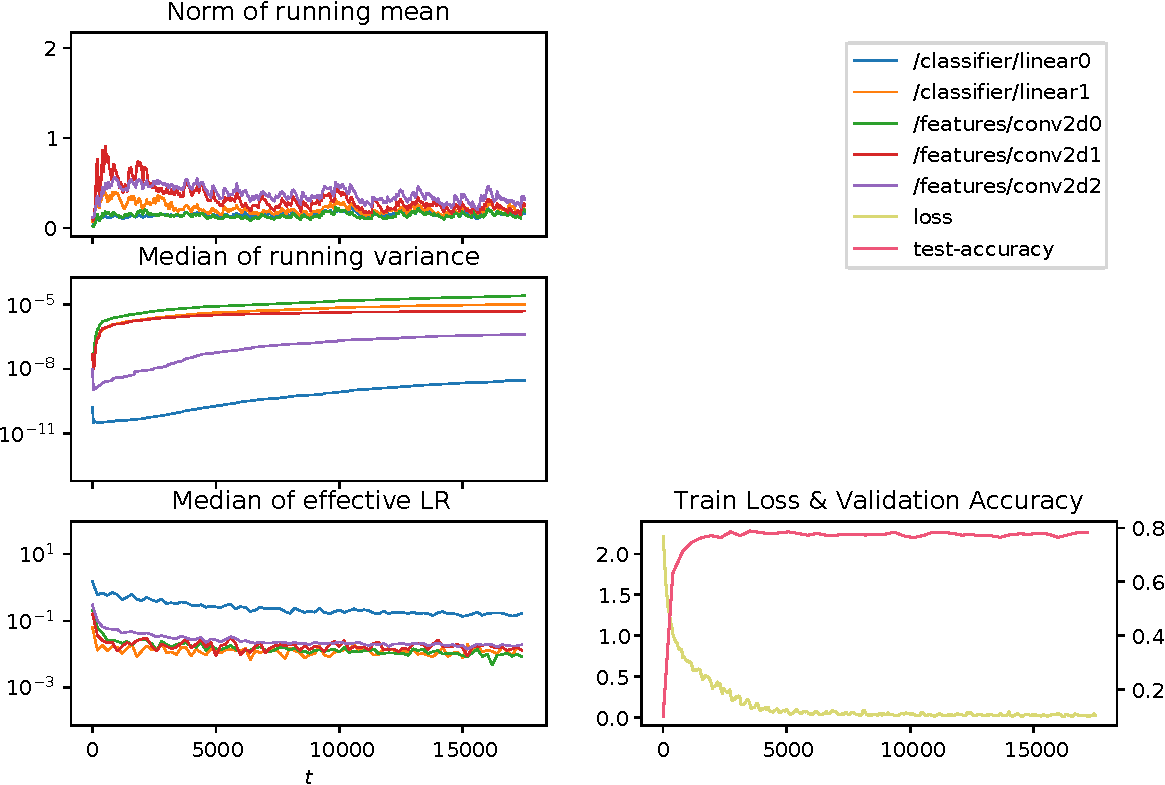
\includegraphics[width=\linewidth]{gfx/diagrams/experiments/adam/adammodel_adam_00005_0_-1.pdf}
        \caption{Adam convnet with learning rate $0.0005$}
    \end{subfigure}

    \begin{subfigure}{\textwidth}
        \centering
        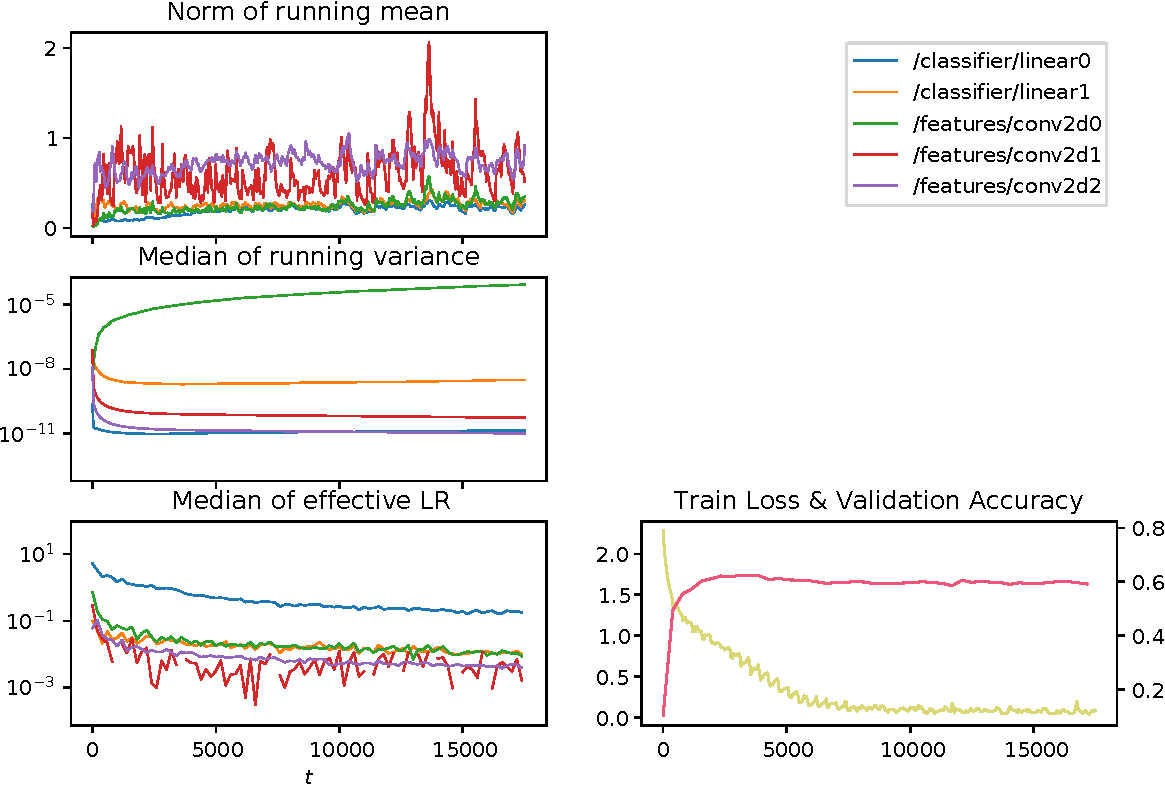
\includegraphics[width=\linewidth]{gfx/diagrams/experiments/adam/adammodel_adam_0001_0_-1.pdf}
        \caption{Adam convnet with learning rate $0.001$}
    \end{subfigure}

    \begin{subfigure}{\textwidth}
        \centering
        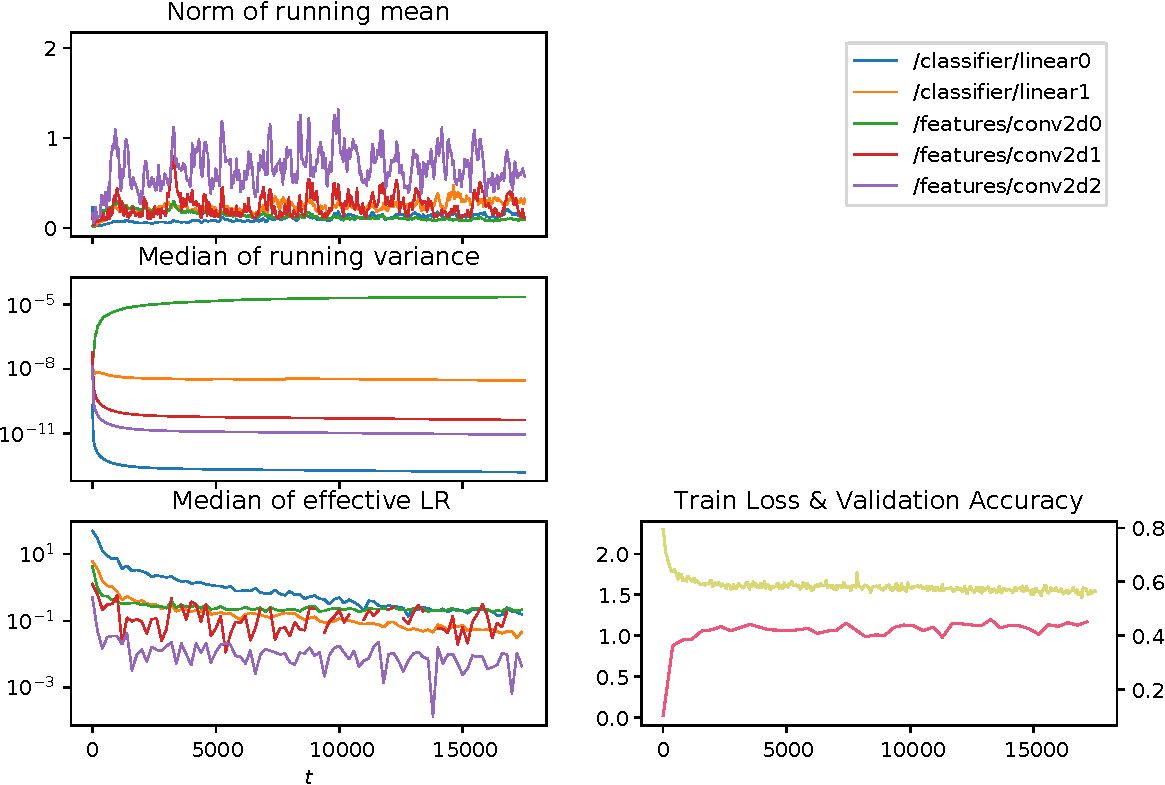
\includegraphics[width=\linewidth]{gfx/diagrams/experiments/adam/adammodel_adam_001_0_-1.pdf}
        \caption{Adam convnet with learning rate $0.01$}
        \label{fig:adammodel-3}
    \end{subfigure}
    \label{fig:adammodel}
\end{figure}

If we consider the SGD algorithm instead (\cref{fig:adammodel-sgd}), we can see
however, that the variance estimate does not vanish in any of the cases, but
instead approaches its asymptote more quickly with increasing learning rate.
This paired with the insights from \cref{fig:adammodel} hints at the importance
of increasing gradient variances in some fashion througout training. Possibly,
an increase in variance is correlated with layers becoming more differentiated
and sensitive to more patterns and is thus indicative of learning progress.
It would be interesting to perform these same experiments with batch
normalisation applied between layers to see whether their influence---which
should counteract any variance increase---invalidates this hypothesis.

\begin{figure}
    \begin{subfigure}{\textwidth}
        \centering
        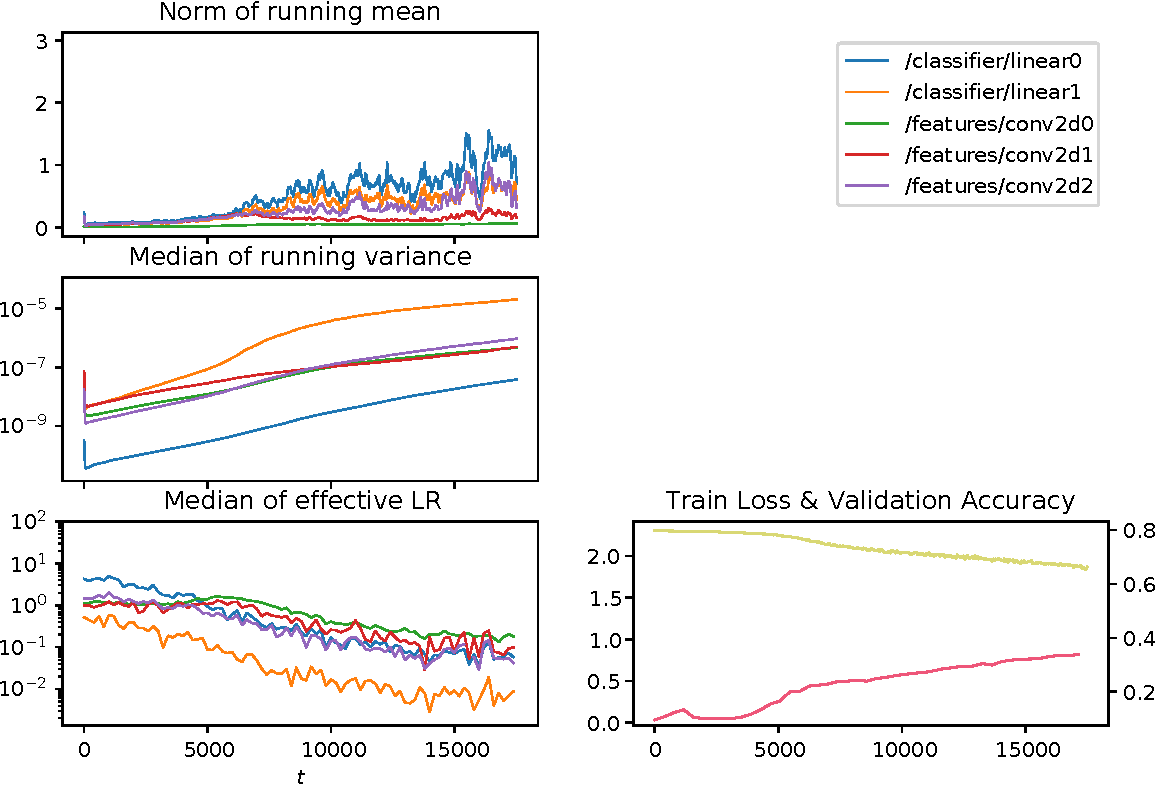
\includegraphics[width=\linewidth]{gfx/diagrams/experiments/adam/adammodel_sgd_00005_0_-1.pdf}
        \caption{Adam convnet with learning rate $0.0005$, optimised with SGD}
    \end{subfigure}

    \begin{subfigure}{\textwidth}
        \centering
        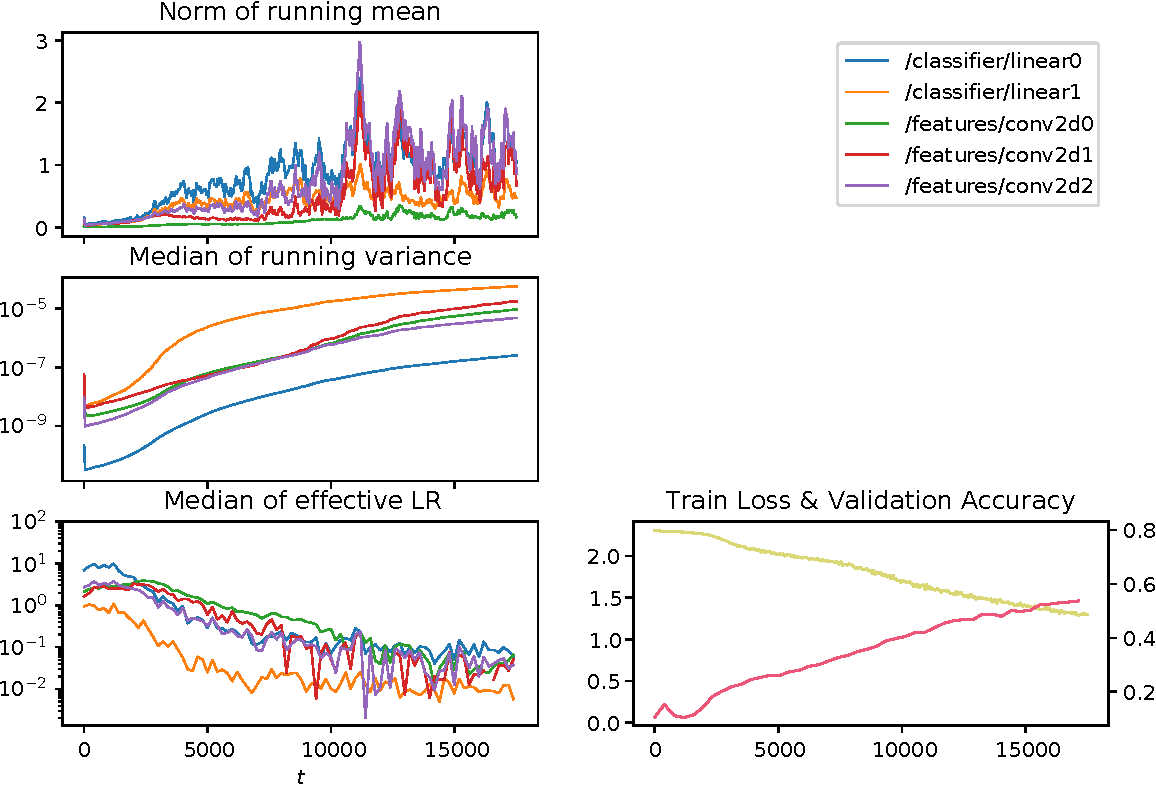
\includegraphics[width=\linewidth]{gfx/diagrams/experiments/adam/adammodel_sgd_0001_0_-1.pdf}
        \caption{Adam convnet with learning rate $0.001$, optimised with SGD}
    \end{subfigure}

    \begin{subfigure}{\textwidth}
        \centering
        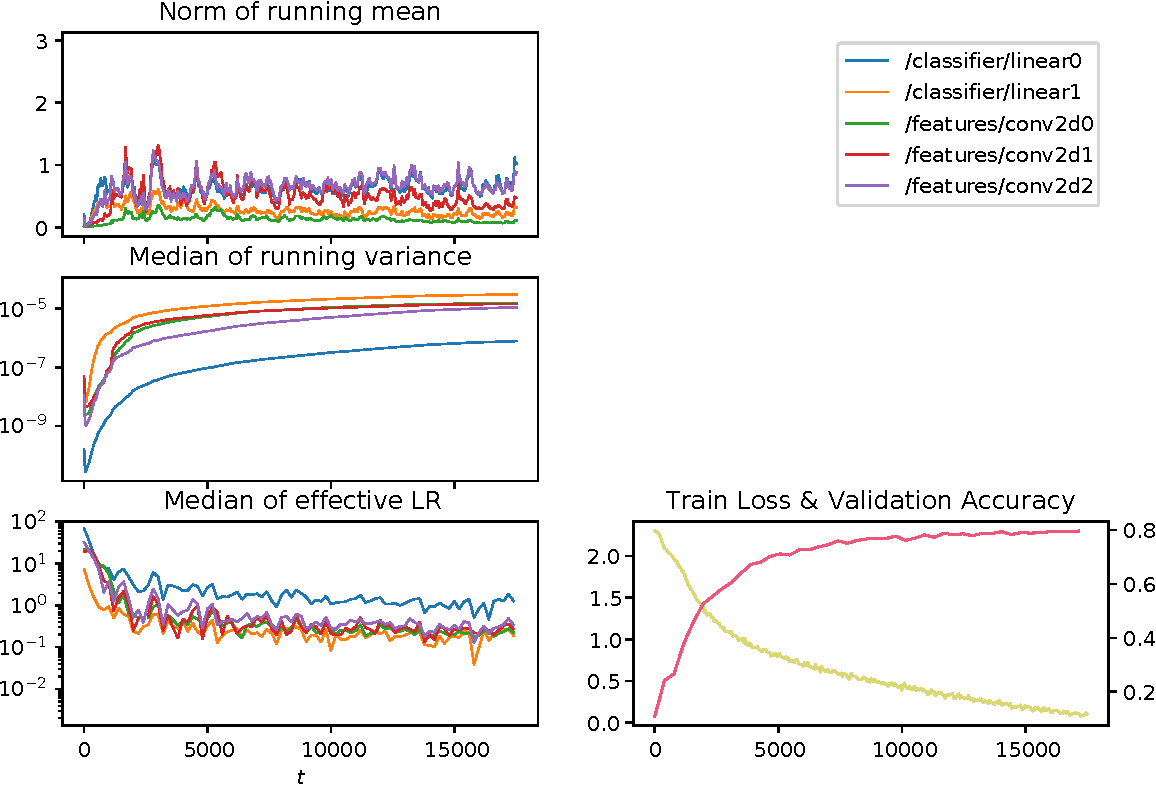
\includegraphics[width=\linewidth]{gfx/diagrams/experiments/adam/adammodel_sgd_001_0_-1.pdf}
        \caption{Adam convnet with learning rate $0.01$, optimised with SGD}
        \label{fig:adammodel-3}
    \end{subfigure}
    \label{fig:adammodel-sgd}
    \caption[Adam moments with SGD]{Adam moments with SGD. The effective learning rate is not used, but
    is what would be used in the Adam update.}
\end{figure}

The experiments above where run on the fully connected model as well (see
\cref{fig:fully-connected}). The results are shown in
\cref{fig:fully-connected-experiment}. The first thing we notice is that Adam
behaves very differently in the absence of convolutional layers. Whereas we saw
a difference in performance between learning rates of $0.0005$ and $0.001$ on
the Convnet, the fully connected model behaves identically in both cases.
\citeauthor{kingma2014adam} state that there is a qualitative difference between
the gradients of dense and convolutional layers, and we see this fact
demonstrated here, as the learning rate does not seem to affect the gradient
distributions much, in contrast with the previous experiment.

Similarly to earlier findings, we see again that Adam is in fact quite sensitive
to the base learning rate set. Once again, a value of one order of magnitude
beyond the best one makes performance deteriorate. In this case, the first
moment estimate vanishes completely, leading to zero-valued gradients and no
learning at all.

\begin{figure}
    \begin{subfigure}{\textwidth}
        \centering
        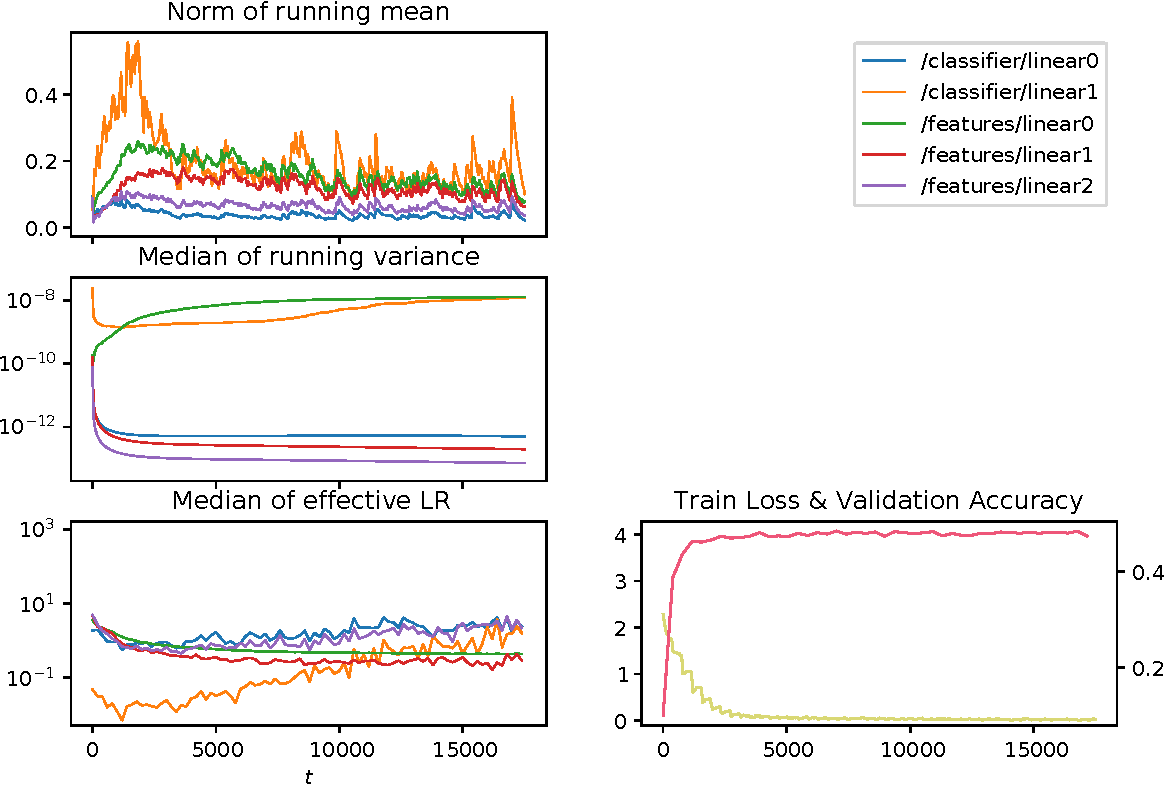
\includegraphics[width=\linewidth]{gfx/diagrams/experiments/adam/fullyconnectedmodel_adam_00005_0_-1.pdf}
        \caption{Dense model with learning rate $0.0005$, optimised with Adam}
    \end{subfigure}

    \begin{subfigure}{\textwidth}
        \centering
        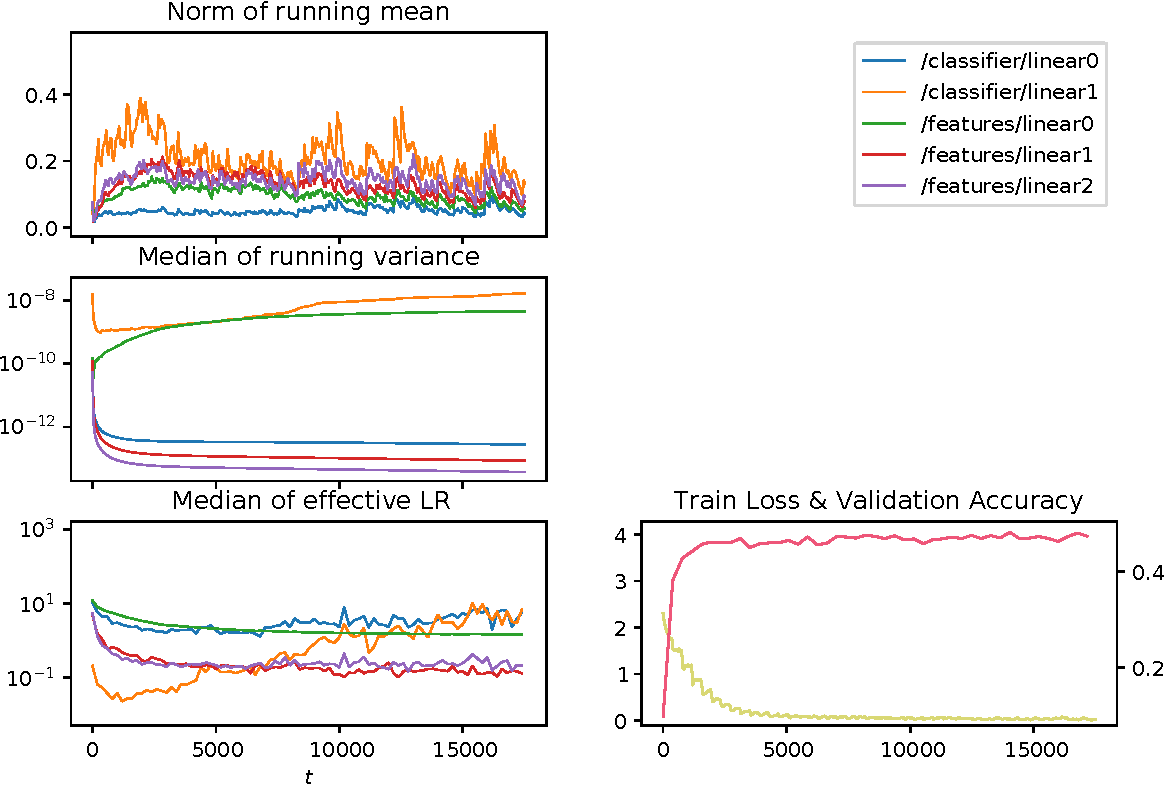
\includegraphics[width=\linewidth]{gfx/diagrams/experiments/adam/fullyconnectedmodel_adam_0001_0_-1.pdf}
        \caption{Dense model with learning rate $0.001$, optimised with Adam}
    \end{subfigure}

    \begin{subfigure}{\textwidth}
        \centering
        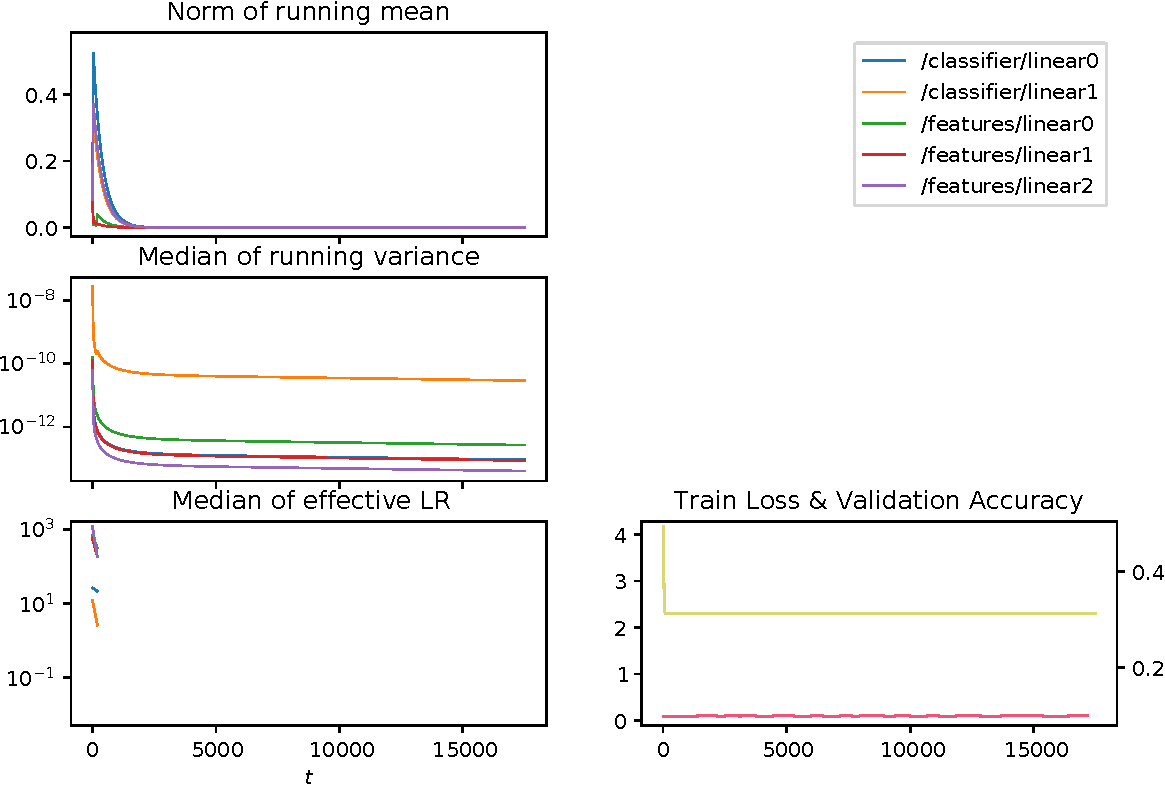
\includegraphics[width=\linewidth]{gfx/diagrams/experiments/adam/fullyconnectedmodel_adam_001_0_-1.pdf}
        \caption{Dense model with learning rate $0.01$, optimised with Adam}
    \end{subfigure}
    \label{fig:fully-connected-experiment}
    \caption{Adam moments on a purely dense model}
\end{figure}

One question not answered yet is \cref{itm:adam-claim-1}. From
\cref{fig:adammodel} and \cref{fig:fully-connected-experiment} we clearly see
that Adam does in fact tend to assigning higher learning rates to dense layers
and lower ones to convolutions. If this heuristic were to be used for manually
tuning SGD, it would indeed be automatically handled by Adam. Ignoring the final
classification layer (\texttt{/classifier/linear1}) in the Convnet, this seems
to come from the fact that dense layers exhibit a gradient variance several
orders of magnitude smaller, while the gradient mean---while still being
smaller---differs by less than one order of magnitude.

We omit here the results for the fully connected model trained with SGD (because
it learns only for the largest learning rate), as well as the larger VGG16
convolutional architecture trained with both optimisers, since the latter
appears to be invariant to any change and may simply be too powerful to exhibit
large differences. See \cref{ch:appendixC} for these experiments.

\subsection{Summary}

With the experiments performed here, we have evaluated the qualitative behaviour
of the Adam optimisation algorithm compared to vanilla stochastic gradient
descent on three architectures, with several learning rates. We find that Adam
is---in spite of its promise---very sensitive to the learning rate and the
correct order of magnitude must be determined beforehand. We have validated that
it automatically assigns smaller learning rates to convolutional layers than to
dense once, a finding in line with a popular heuristic employed manually for
SGD. We also examined the behaviour of the second moment estimate and find that
it appears to be related to the speed of learning, albeit not in a trivial
fashion. A further interesting phenomenon is that median learning rates for
individual layers can range from $10^{-3}$ all the way up to $10$, which would
never work when applied to an entire network. More work would be necessary to
check whether using these learning rates for SGD would achieve the same
performance. If not, then this would prove that Adam finds qualitatively
different paths through the weight space by incoporating past gradient
information. Reason to believe that this is indeed the case is supported by
\citet{NIPS2018_7815} who find that the representations learned by the same
network with different learning rates are qualitatively different.

The \texttt{ikkuna} library was used to extract all metrics during training and
log them to a database. While code for the experimental setup had to be written,
the code for computing and logging the metrics is simple and short, and only
needs to be written once. This software could have been used to easily perform
more experiments than \citet{kingma2014adam} provided.

\section{Detecting Learning Rate Problems}%
\label{sec:detecting_learning_rate_problems}

\subsection{Ratio-Adaptive Learning Rate Scheduling}%
\label{sub:ratio_adaptive_learning_rate_scheduling}

The first problem to be investigated is that of choosing an appropriate learning
rate. We begin with a brief review of gradient descent and then evaluate how
the update-to-weight ratio of model weights can be used to identify bad learning
rates or automate learning rate selection.

As a first hypothesis, we investigate a claim made by \citet{karpathycs231n} who
states that the ratio between updates and weights is a quantity which should be
monitored and constrained. He suggests a target of $\frac{1}{t} = 10^{-3}$ as a
reasonable value, but to the author's knowledge there has never been a thorough
investigation of this hypothesis. Because of this lack of exploration and the
celebrity of the proponent, this merits further investigation.

It seems intuitive that this target cannot be static throughout training, since
we usually decay the learning rate towards the end, leading to smaller magnitude
of updates (this is a prerequisite for theoretical convergence guarantees for
SGD, see \citet[p. 20]{saad1998online}). As a matter of fact, this can be easily
verified by running training with an update rule that scales each gradient so
that the update hits the target (the network does learn, but to a significantly
smaller final accuracy; see \cref{fig:fixed-ratio-opt}). It is also not clear
whether the target should apply to all layers equally, since this would
constitute a strong regulariser on the network parameters, limiting
expressiveness of the model. For instance, in networks with the (now outdated)
$\text{tanh}$ activation function, the later layer's gradients are larger as
fewer backpropagation steps have been done to them, and for this activation
function at least, each application of the chain rule entails multiplication
with a factor $< 1$ (as the tanh derivative never exceeds $1$ and decreases to
almost $0$ in both limits), so gradients become exponentially small. In fact,
the vanishing gradient problem was the main driver to introduce non-saturating
activation functions.  Other nonlinearites such as the rectified linear unit do
not exhibit the same behaviour, but that does not mean all layers must change at
the same rate.

\begin{figure}
    \centering
    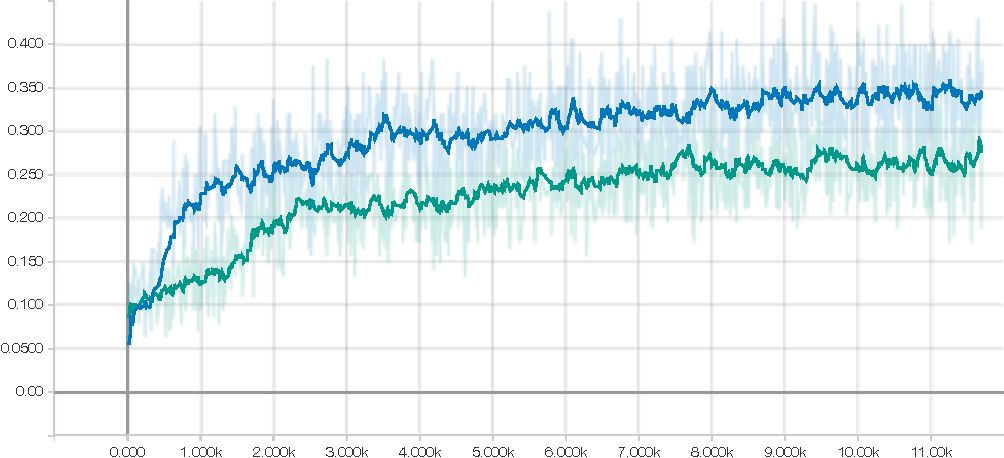
\includegraphics[width=\linewidth]{gfx/diagrams/experiments/ratio_loss_correlation/alexnetmini_sgd_fixed_ratio_01.pdf}
    \caption[Fixed-Ratio optimisation with AlexNetMini on CIFR10]{AlexNetMini on CIFAR10 at $0.1$ learning rate. The blue line is
    vanilla SGD while the green one is obtained by scaling the gradients to have
the updates meet a target ratio of $10^{-3}$.}
    \label{fig:fixed-ratio-opt}
\end{figure}

As a first approach to an evaluation, we want to try and select the learning
rate in such a way as to hit the target postulated by
\citeauthor{karpathycs231n}, but not precisely for each layer, but on average
over all layers. This would allow for more flexibility in the weight updates
compared to fixing each update to the same value.

The experimental setup uses the simplified AlexNet architecture
(\cref{sec:pack-models}) shown in \cref{fig:alexnetmini}. The dataset used is
the well-known CIFAR-10 dataset consisting of $60,000$ $32\times32$ colour images
from ten object categories \citep{krizhevsky2009learning}. The optimisation
algorithm used is plain stochastic gradient descent on minibatches of size $128$. The
dataset does not constitute a hard problem to solve; state of the art accuracies
lie around $95\%$. For this reason, a decision must be made about how to make
the problem hard enough so that improvements to the training schedule can
actually be made. The learning rate has thus been fixed to a high value of $0.2$
which is not the optimal value (a learning rate of $0.1$ solves the problem to
$45\%$ accuracy).

\begin{figure}
    \centering
    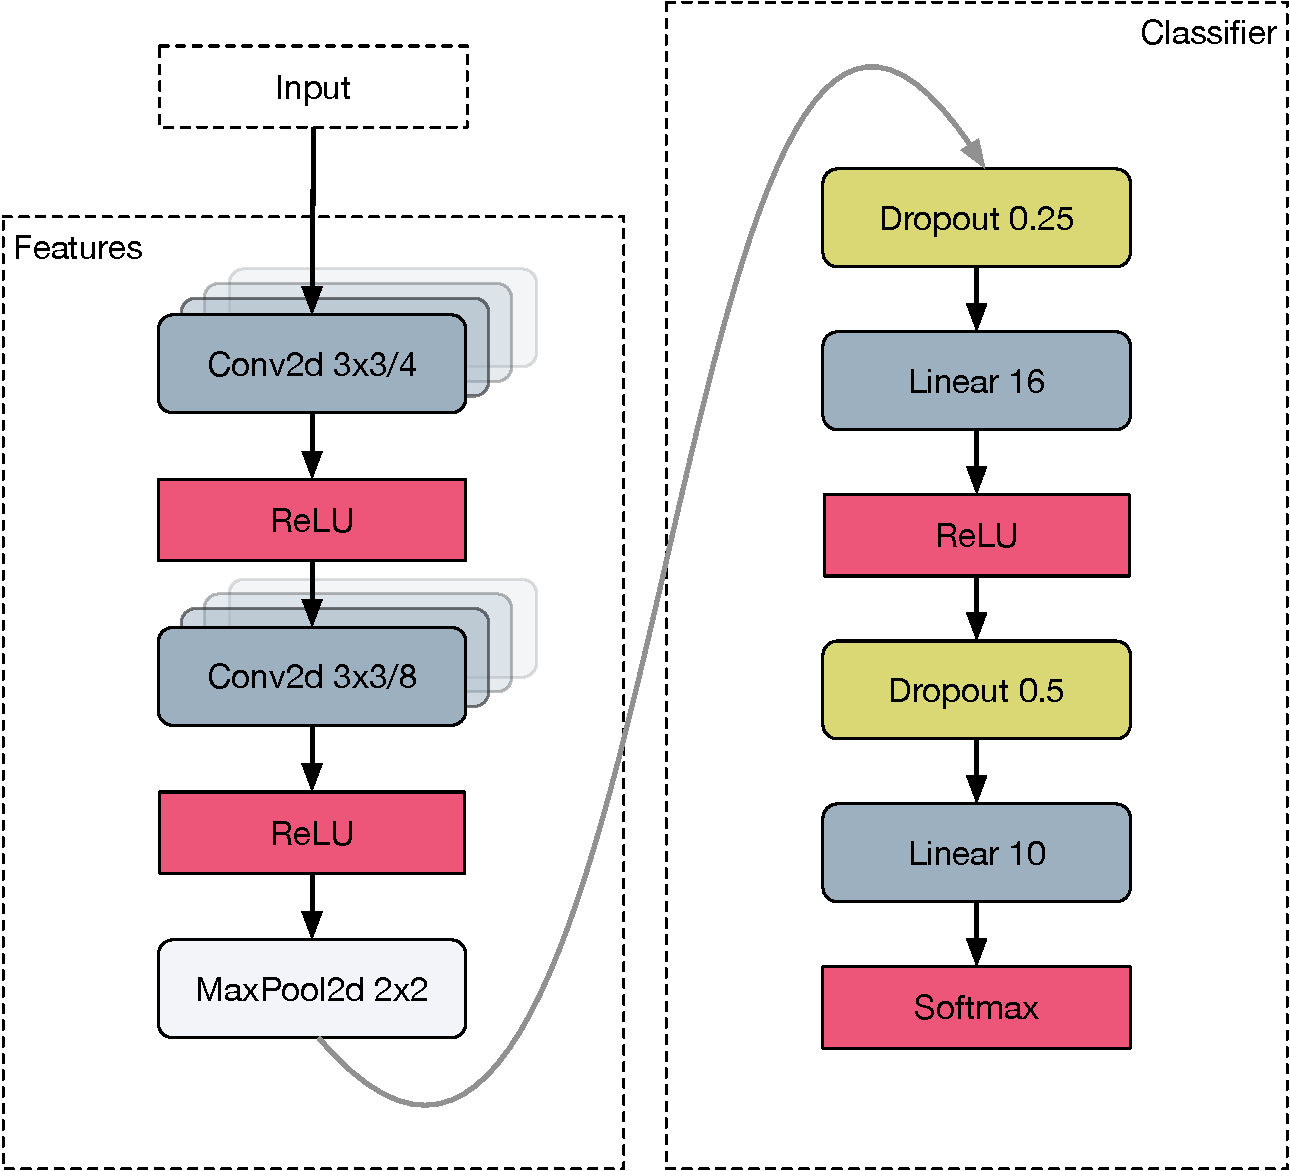
\includegraphics[width=\linewidth]{gfx/diagrams/neural_network/alexnetmini.pdf}
    \caption[Simplified AlexNet architecture]{The network used in this
    experiment. Image features are extracted by $4$ and $8$ convolutional
    filters, respectively, with ReLU nonlinearities. Maximum pooling is applied
    with a filter and stride size of $2$ leading to a resolution a fourth of the
    original size. The classifier portion employs dropout layers to reduce
    co-adaptation of units and a final softmax activation to map outputs to
    class probabilities in $(0,1)$.}
    \label{fig:alexnetmini}
\end{figure}

In order to validate that there is room for improvement (i.e.~the task is not
too easy), the training has been
run about twenty times for both a constant learning rate and an exponentially
decaying rate according to
\begin{equation}
    \eta_{e+1}  = 0.98^{e+1} \eta_{e},
\end{equation}
$e$ being the epoch index.
The final accuracies after $100$ epochs of training for constant learning rate,
exponential decay are shown in \cref{fig:validation1}. As can be seen, there is
a significant improvement when decaying the learning rate over keeping it
constant.

\begin{figure}
    \centering
    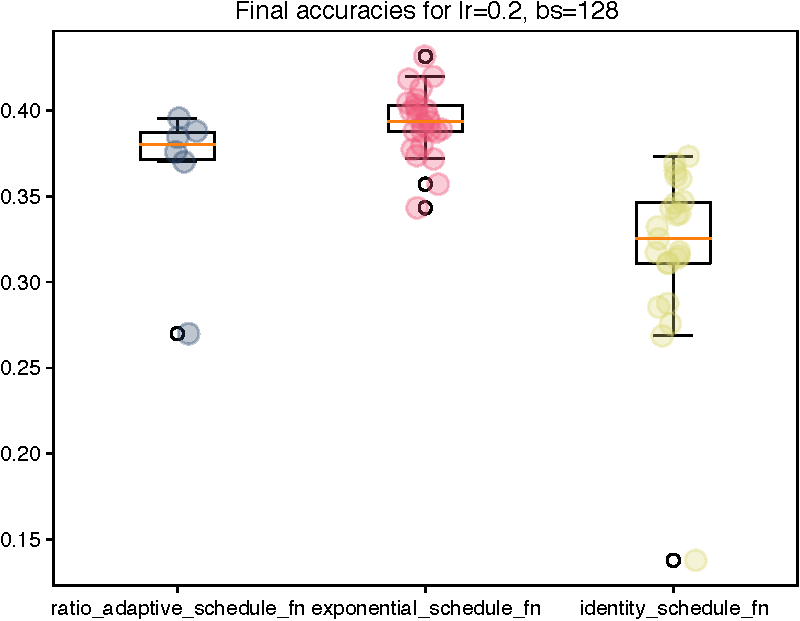
\includegraphics[width=\linewidth]{gfx/diagrams/experiments/experiment_validation.pdf}
    \caption[Final accuracies after 100 epochs]{Final accuracies after 100
    epochs with a learning rate of $0.2$ and batch size of $128$. The adaptive
    ratio schedule is discussed in\cref{sec:ratio-schedule}}
    \label{fig:validation1}
\end{figure}

\subsubsection{The Adaptive Update-to-Weight-Ratio Schedule}\label{sec:ratio-schedule}%

As a first showcase of the library and a test of the update-weight ratio
hypothesis, an adaptive learning rate based on the aforementioned ratio is
implemented with the help of the library.  We will start by formally describing
the update rule and then show how it is implemented with \texttt{ikkuna}.

Let $l$ be the number of layers with weight matrices associated with them (for
instance linear or convolutional layers, but not activation functions, dropout,
or the like). Let $\left\{W_{i,k} \mid i = 0 \ldots l - 1\right\}$ be the set of weight
matrices at training step $k$.  Let $\eta$ be the base learning rate and
$\frac{1}{t}$ be a target value to which we want the update-to-weigh ratio to
move. Furthermore, let $\gamma \in (0, 1)$ be a decay factor for exponential
smoothing.  Now, let

\begin{equation}
    R_{i,k} = \frac{||W_{i,k} - W_{i,k-1}||_2}{||W_{i,k}||_2}
\end{equation}
be the ratio between the $L2$-Norms of layer $i$'s weight updates before step $k$ step
and the weights at step $k$ themselves.  We then select the new learning rate
for batch step $k+1$ as

\begin{align}
    \eta_{k+1}   = \eta_{k}
                   \left(
                   t \cdot \frac{1}{l}
                   \sum_{i=0}^{l-1} \gamma R_k + (1 - \gamma) R_{k-1}
                   \right)^{-1}
\end{align}
for $k \ge 2$.  This is the average exponentially smoothed update-weight-ratio,
divided by the target range. This learning rate is used for vanilla gradient
descent without any other modifications beyond capping it to some value in case
of very small ratios. The effect of adapting the learning rate according to this
schedule is that the average ratio between the weight updates and the weights
moves towards the target range.  It should be noted that this update rule biases
the learning rate in favour of the smaller layers since all ratios are weighted
equally, regardless of the number of weights.
\Cref{fig:schedule-accuracies} displays a set of accuracy traces for each of the
schedules (constant, exponential decay, ratio-adaptive) with different base
learning rates. The network was trained from scratch $5$ times for each combination.

\begin{figure}
    \centering
    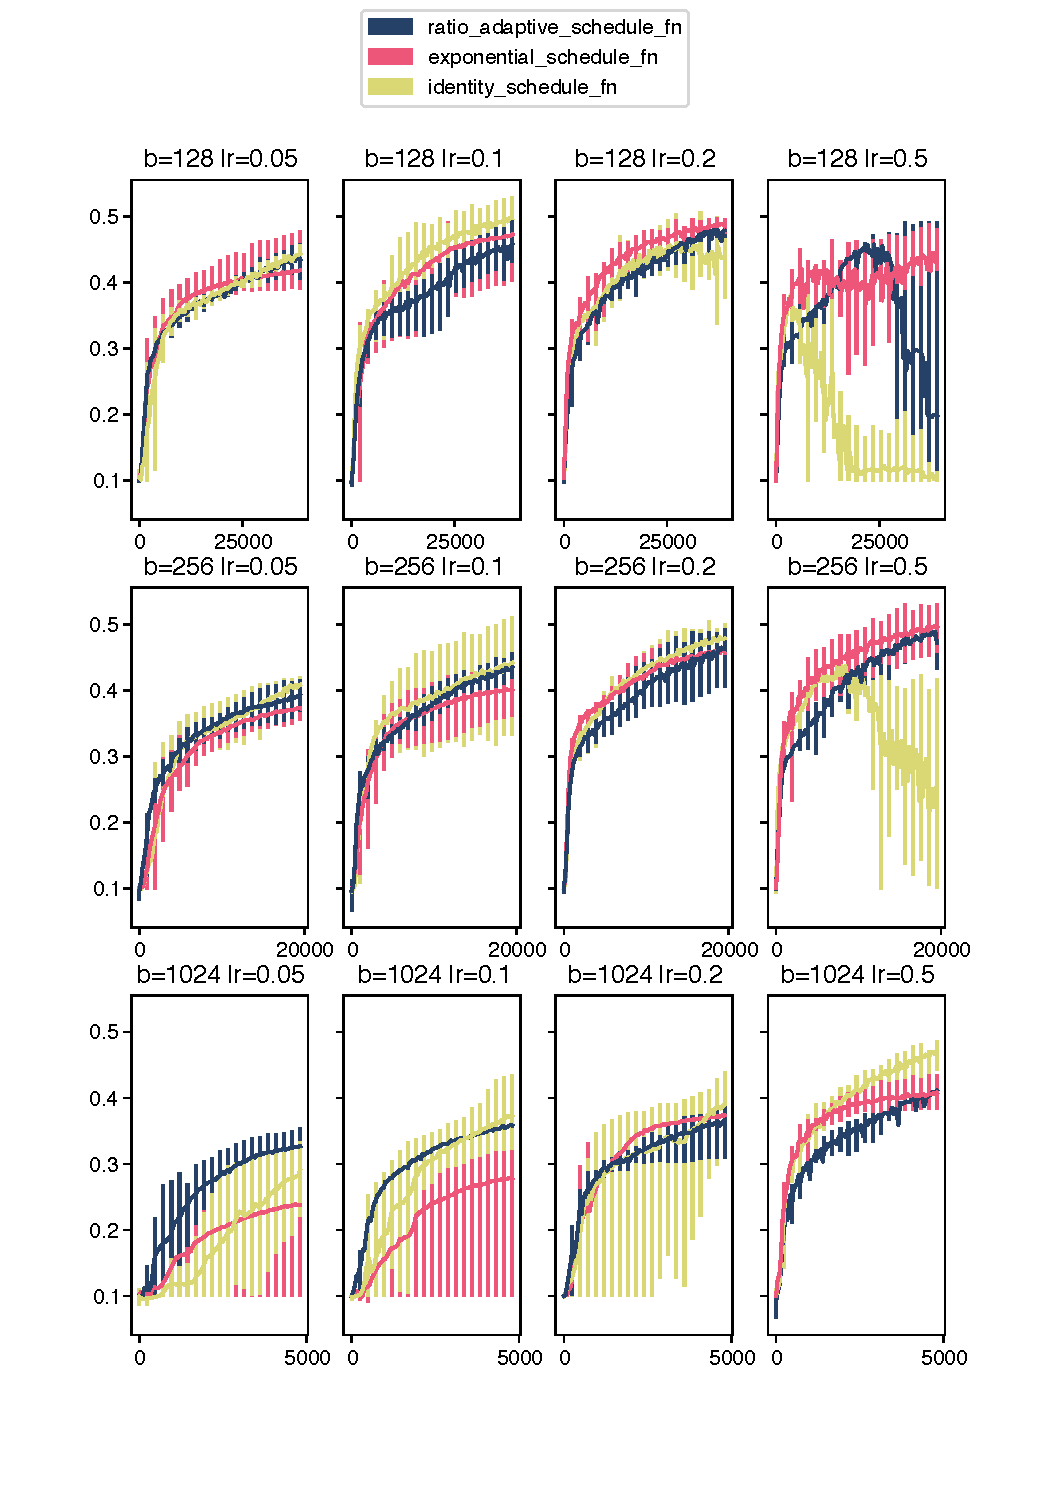
\includegraphics[width=\linewidth]{gfx/diagrams/experiments/ratio_adaptive_accuracies.pdf}
    \caption[Accuracy traces for different schedules on CIFAR-10]{Accuracy traces
    for different schedules on CIFAR-10. Batch size and initial learning rate are
    shown above each subplot. The exponential decay schedule uses a decay factor of
    $0.98$. Chance level is $0.1$. The experiments are run for $100$ epochs
    each.}
    \label{fig:schedule-accuracies}
\end{figure}

The results are not overwhelming, which is unsurprising for such a
simple schedule. For the smaller learning rates, it is not better or worse than
a constant or exponentially decaying schedule. However, for unnecessarily high
learning rates, the adaptive schedule outperforms the constant one, hinting at a
possible signal for identifying too high learning rates. This holds for the
smaller of the three batch sizes, which makes sense as a high batch size is
generally more amenable to a high learning rate, as the larger sample size
reduces the noise in the gradient and makes for a smoother loss landscape as the
gradients for more samples are averaged. On the other hand, the adaptive schedule
is also better than a constant one for very small learning rates on large batch
sizes. So it not only works in preventing too-high learning rates, but also too
low ones. This signal could hence be useful for
identifying inappropriate learning rates in small or large batch sizes.

As an impression of how the library presented in \cref{ikkuna} simplifies a
general implementation of such a learning rate schedule, code is provided here.

When an \verb+Exporter+ is configured for a given model, a
\verb+RatioSubscriber+ (see \cref{tbl:subscribers}) must be added to the message
bus in order for the update-weight-ratio ($R_{i,k}$ in the above equations) to be
published. One can then subscribe them and process the information with this
subscriber:
\begin{lstlisting}
class RatioLRSubscriber(PlotSubscriber):
    def __init__(self, base_lr, smoothing=0.9, target=1e-3, max_factor=500):
        subscription = Subscription(self, ['weight_updates_weights_ratio', 'batch_started'],
                                    tag=None, subsample=1)
        super().__init__([subscription], get_default_bus(),
                         {'title': 'learning_rate',
                          'ylabel': 'Adjusted learning rate',
                          'ylims': None,
                          'xlabel': 'Train step'})
        # exponential moving avg of R_{i,k}
        self._ratios     = defaultdict(float)
        # maximum multiplier for base learning rate (in pathological cases)
        self._max_factor = max_factor
        # exp smoothing factor
        self._smoothing  = smoothing
        # target ratio
        self._target     = target
        # this factor is always returned to the learning rate scheduler
        self._factor     = 1
        self._base_lr    = base_lr

    def _compute_lr_multiplier(self):
        '''Compute learning rate multiplicative. Will output 1 for the first batch since no layer
        ratios have been recorded yet. Will also output 1 if the average ratio is close to 0.
        Will clip the factor to some max limit'''

        n_layers = len(self._ratios)
        if n_layers == 0:   # before first batch
            return 1
        else:
            mean_ratio = sum(ratio for ratio in self._ratios.values()) / n_layers
            # prevent numerical issues and keep current LR in that case
            if mean_ratio <=  1e-9:
                return 1
            else:
                factor = self._target / mean_ratio
                return min(factor, self._max_factor)

    # invoked by the runtime for each incoming message
    def compute(self, message):
        if message.kind == 'weight_updates_weights_ratio':
            # the `key` property for these messages will be the module/layer
            # here we compute the exponential moving average of ratios
            i               = message.key
            R_ik            = message.data
            R_ik_1          = self._ratios[i]
            gamma           = self._smoothing
            self._ratios[i] = gamma * R_ik + (1 - gamma) * R_ik_1
        elif message.kind == 'batch_started':
            # before a batch starts, update the lr multiplier
            self._factor = self._compute_lr_multiplier()

    def __call__(self, epoch):
        return self._factor
\end{lstlisting}

The subscriber implements the \verb+__call__()+ method so it can be dropped into
PyTorch's learning rate scheduler (\verb+torch.optim.lr_scheduler.LambdaLR+).
This learning rate schedule can thus be used in every model, without modification.


\subsection{Effects Of Update-to-Weight-Ratio On Training Loss}%
\label{sub:effects_update_to_weight_ratio_on_training_loss}

We have seen in the previous section that at least for pathological cases the UW
ratio can be used to correct the learning rate to some extent. In this section,
we want to examine how this ratio does or should change during training. As
discussed in \cref{sub:ratio_adaptive_learning_rate_scheduling}, it is unlikely
that a constantly high rate of change to the weights will be beneficial
throughout the entire training. We would therefore like to find a relation
between the loss decrease, the current UW ratio and the point in time during
training. This could help us improve the learning rate schedule developed above
and refine the use of the UW ratio as a signal for inappropriate learning rates.

For this experiment, we learn CIFAR-10 for $75$ epochs, again with a batch size
of $128$, with vanilla SGD and the Adam optimizer and different learning rates.
We use the AlexNetMini architecture again, as well as a larger, more powerful
VGG network (schema in \cref{fig:vgg16}). We employ \verb+ikkuna+ to record
losses, accuracies and UW ratios for each layer automatically during training.
In order to make larger trends visible, we smooth the loss trace with a gaussian
kernel.

\begin{figure}
    \centering
    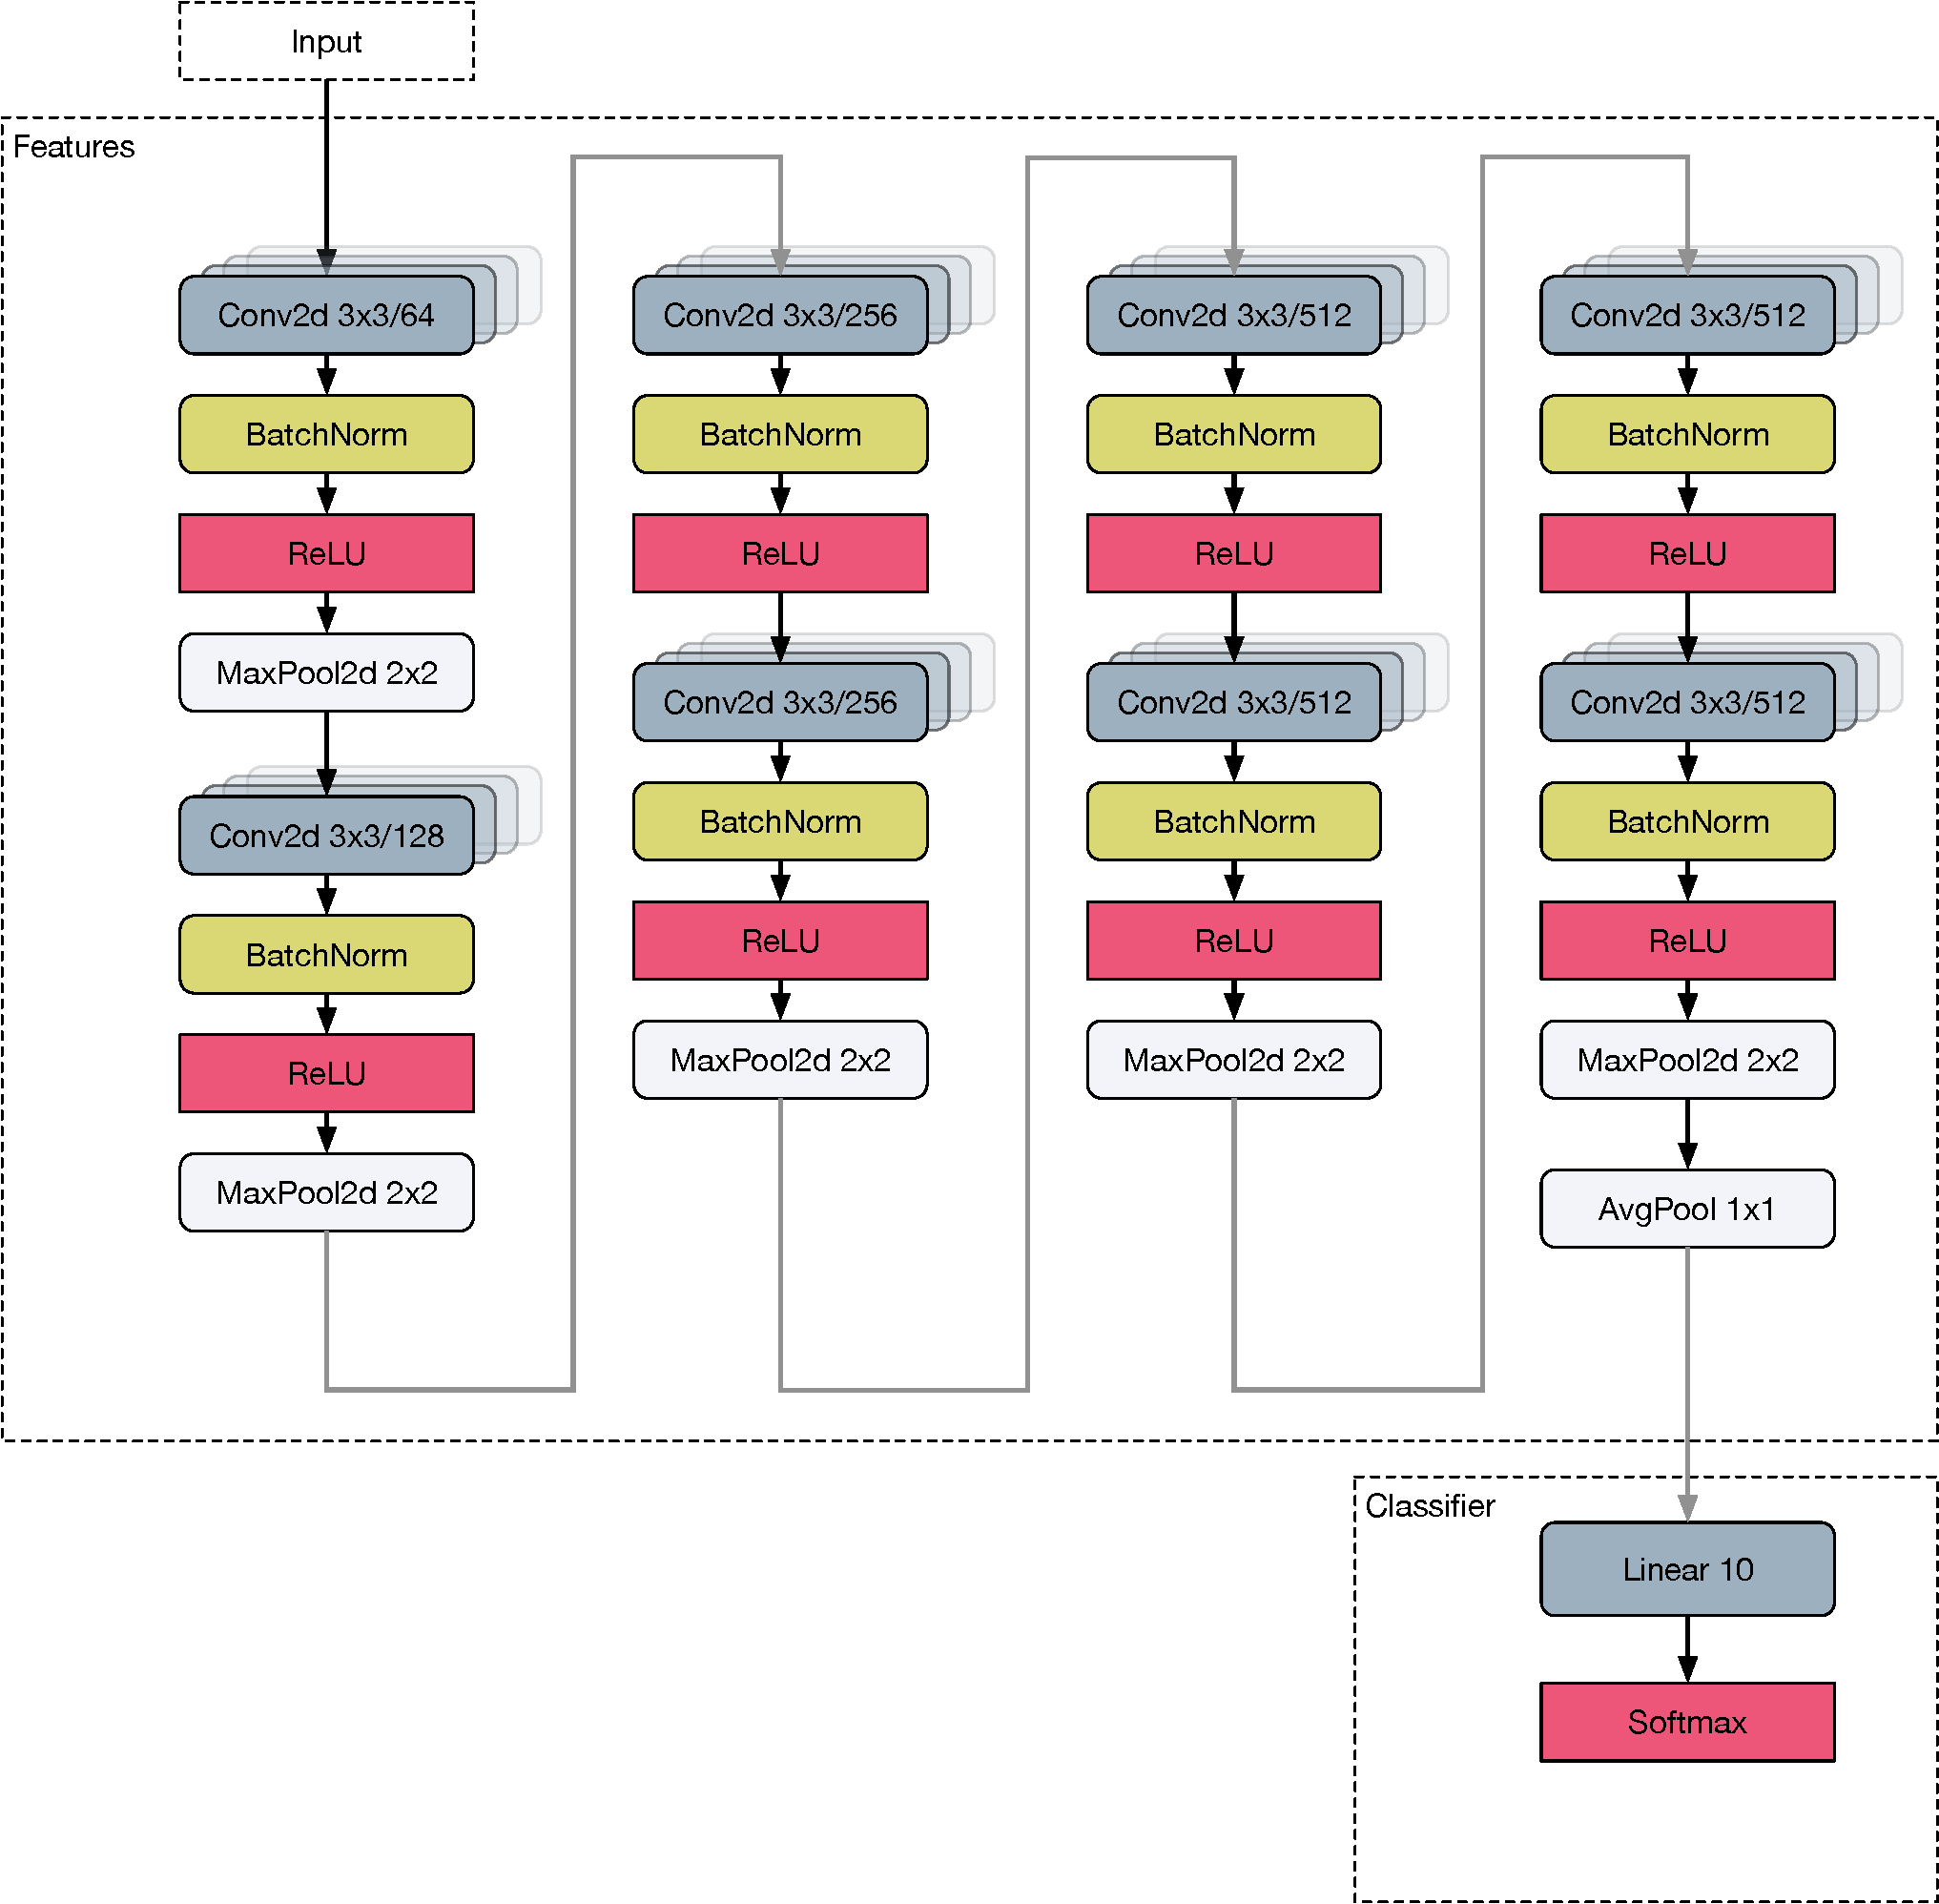
\includegraphics[width=\linewidth]{gfx/diagrams/neural_network/vgg.pdf}
    \caption[VGG network with $8$ convolutionsl layers.]{VGG network with $8$ convolutional layers.}
    \label{fig:vgg16}
\end{figure}

In the following figures, we plot the loss traces and their negative
derivative\footnote{Erratum: The plots incorrectly refer to the ``inverse``
derivative.}
(the amount of decrease) in the upper right, the average weight-update ratio in
the lower right, and a scatter plot of ratio versus loss decrease on the left.
The scatter plot has the time step colour-coded (blue is early, red is late) and
in addition offsets according to time on the $z$-axis. Due to the number of
points (up to $30,000$ time steps times the number of runs), the plots have been
subsampled where many points overlap. This was necessary to render the data for
this document. Care has been taken to not destroy the topology of the data.  The
density in a given area may thus not be entirely accurate. In the UW ratio
plots, the line displayed is the average over multiple runs.

\subsubsection{VGG with Stochastic Gradient Descent}

The plots in for this network only show the first $10,000$ training steps since
nothing of note happens afterwards. Since most of the ratio values cluster
around the same values towards the end of training, logarithmic subsampling was
applied.  For the VGG network, we observe a smooth decrease in the training loss
alongside a decrease in the average update-to-weight ratio. Training basically
stalls after around $10,000$ steps (about $25$ epochs).  We observe the trend
that the UW ratio is initially fairly high and falls off subsequently, which
correlates with a decrease in loss. However, there is no particular value of the
ratio that exhibits any significant correlations beyond other values. The
ratio in the beginning of training is also proportional to the learning rate, as
is to be expected.

It is curious that in the very beginning of training, the UW ratio has the
highest value, but the decrease in loss for these steps increases throughout the
first few batches (i.e. learning accelerates) before tapering off. This is
barely visible in the line plots, but shows as a prominent feature in the
scatter plot. It should be noted that this phenomenon happens on a very small
timescale---the number of data points in the arc is orders of magnitude smaller
than in the rest of the plot, therefore it is no more than a curiosity. As a
preliminary conclusion, we can affirm that there is no linear correlation
between the ratio and the decrease in loss.

Furthermore, the smallest of the evaluated learning rates converges fastest.
The loss flatlines at $0$ after little more than $4,000$ steps, while the larger
learning rates need proportionally more time. The difference is marginal
however. The phenomenon might relate to the motivation for annealing the
learning rate: As we approach a local minimum, we need smaller learning rates to
not jump over it in a different direction in every update, but slowly fall into
the minimum itself instead. This may be an indication that an appropriate learning rate
for this particular problem is $\le 0.01$. None of the configurations exhibit UW
ratios close to Karpathy's suggestion of $10^{-3}$, but with the smallest
learning rate, we get closest, and converge fastest. Perhaps this could motivate
Karpathy's constant.

\begin{figure}
    \begin{subfigure}{\textwidth}
        \centering
        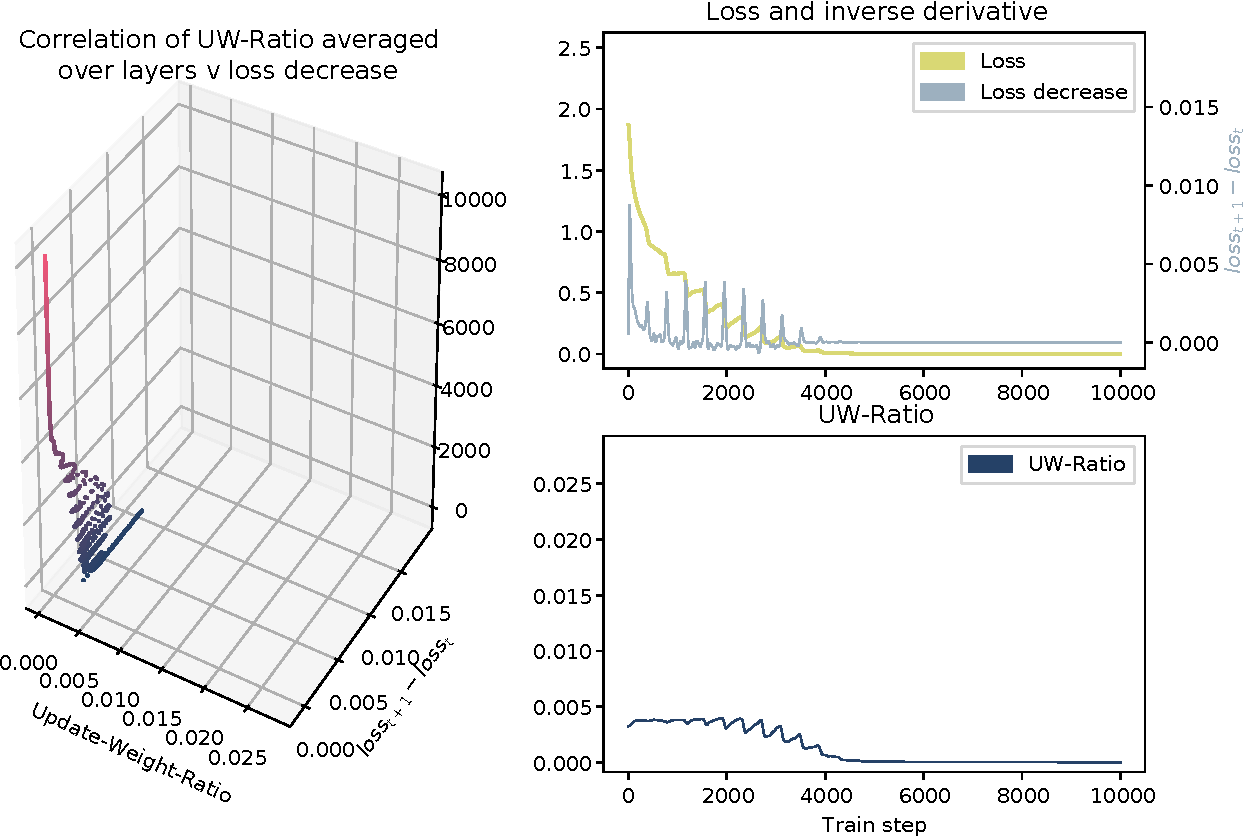
\includegraphics[width=\linewidth]{gfx/diagrams/experiments/ratio_loss_correlation/vgg_sgd_001_0_10000.pdf}
        \caption{UW ratio experiment for VGG with SGD and learning rate $0.01$}
        \label{fig:ratio_loss_corr_vgg_sgd_001}
    \end{subfigure}

    \begin{subfigure}{\textwidth}
        \centering
        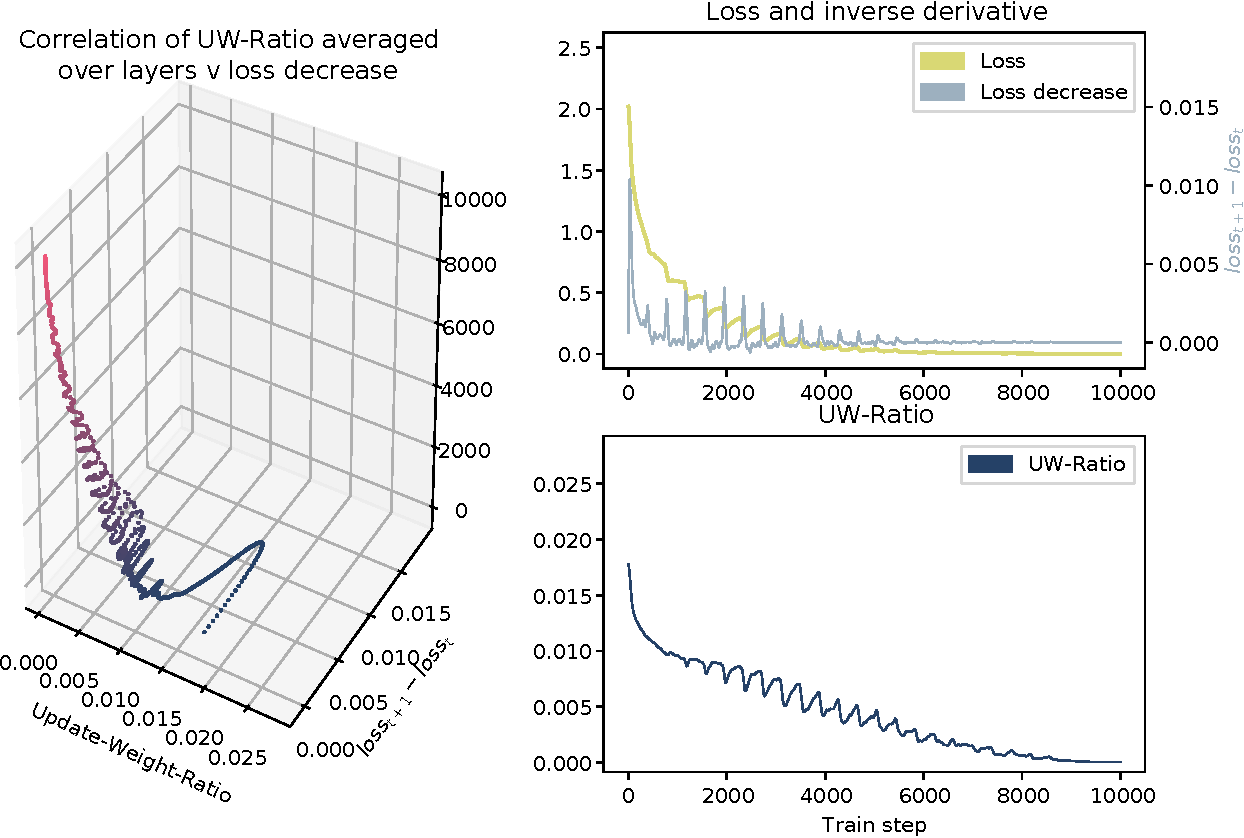
\includegraphics[width=\linewidth]{gfx/diagrams/experiments/ratio_loss_correlation/vgg_sgd_005_0_10000.pdf}
        \caption{UW ratio experiment for VGG with SGD and learning rate $0.05$}
        \label{fig:ratio_loss_corr_vgg_sgd_005}
    \end{subfigure}

    \begin{subfigure}{\textwidth}
        \centering
        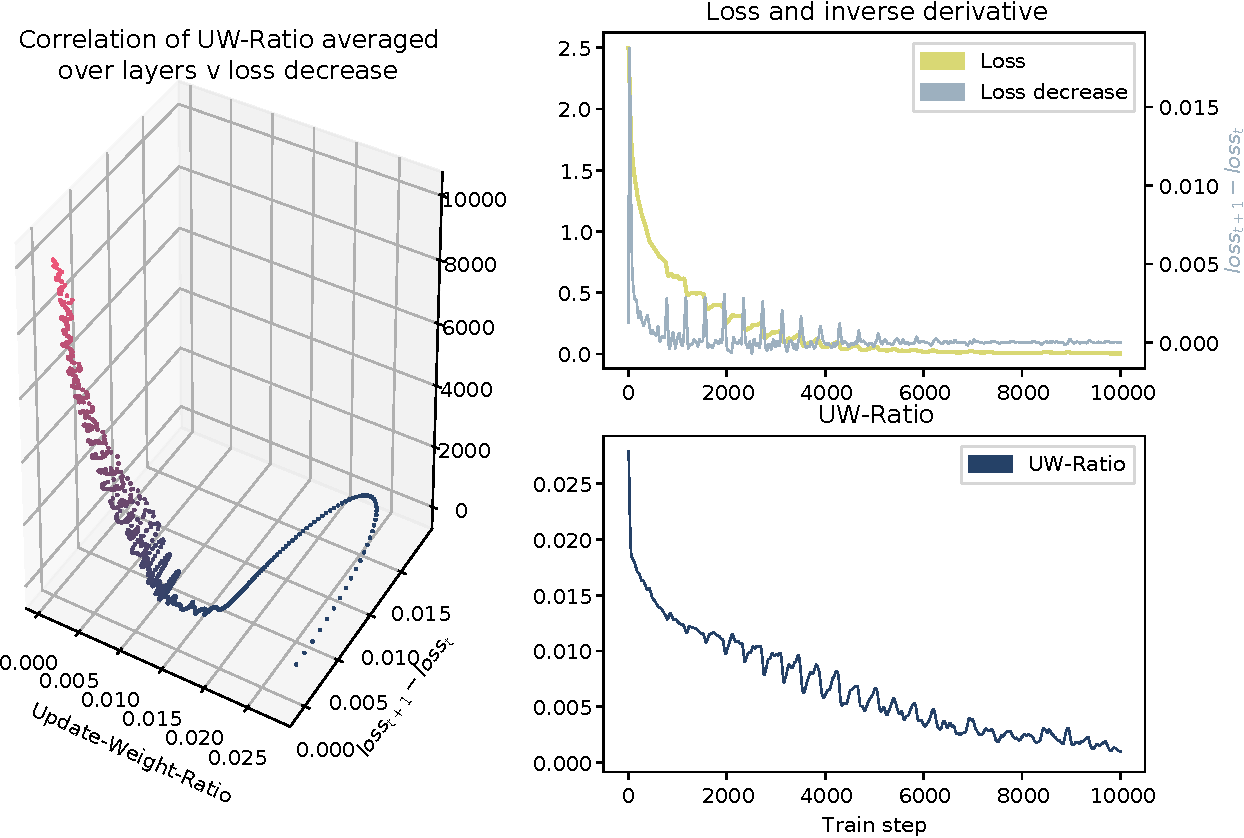
\includegraphics[width=\linewidth]{gfx/diagrams/experiments/ratio_loss_correlation/vgg_sgd_01_0_10000.pdf}
        \caption{UW ratio experiment for VGG with SGD and learning rate $0.1$}
        \label{fig:ratio_loss_corr_vgg_sgd_01}
    \end{subfigure}
\end{figure}

\subsubsection{VGG with Adam}

The same experiment has been run with the Adam optimizer \citep{kingma2014adam}
and has been found to produce quite different results. We mainly observe that
the steplike nature of the loss function (sharp decreases at epoch boundaries)
are much less pronounced with the Adam optimizer. This removes the loops  which we see for
SGD from the scatterplots. In absolute terms, Adam begets a much higher UW ratio
in the beginning of training, which falls off quickly to SGD's values.
Convergence takes minimally longer and doesn't occur at all with a learning rate
of $0.1$ (\cref{fig:ratio_loss_corr_vgg_adam_01}). Counterintuitively, the
adaptive optimiser is unable to adapt to the high learning rate and is
outperformed by vanilla SGD. The Adam optimiser keeps running estimates of the
mean and variance of the gradient of each parameter, with exponential smoothing
applied. The learning rate is adjusted for each parameter by multiplying it with
$\frac{\mu_{\text{grad}}}{\sqrt{\sigma_{\text{grad}}} + \epsilon}$. The argument
by \citet{kingma2014adam} is that in locations of high gradient variance, a
lower learning rate is appropriate since the estimate of the gradient at this
spot is noisy and unreliable, so smaller steps are a safer choice. Furthermore,
they claim that the mean of the gradient vanishes closer to an optimum, which is
also where we need to anneal the learning rate lest we jump over the minimum.
The Adam optimiser thus has learning rate annealing built-in. The step size
parameter $\eta$ is supposed to be of less importance since in Adam's parameter
update rule, it gives an upper bound on the size of the steps taken in parameter
space, but it can always be adjusted downward if the gradient variance is too
high. It can also be adjusted upward up to the upper bound if the gradient mean
is high, giving Adam momentum-like behaviour. The primary proposition of
\citet{kingma2014adam} is that manually tuning the learning rate per layer or
even per parameter is no longer necessary, but we see here that cases can be
found where precisely this behaviour of Adam would be needed---we have set a
too-high learning rate, but Adam fails to compensate for this negligence. This
casts doubt on the universality of the Adam optimiser.\footnote{The hypothesis
that Adam starts to show its merit in the absence of batch normalisation could
not be tested on the VGG architecture, since training did not progress at all
with any learning rate or optimiser when batch normalisation layers were
removed. For the smaller AlexNetMini architecture with added batch
normalisation, Adam did not outperform SGD in the absence of batch norm. To the
contrary, Adam even lead to vanishing gradients when using batch normalisation.}

\begin{figure}
    \begin{subfigure}{\textwidth}
        \centering
        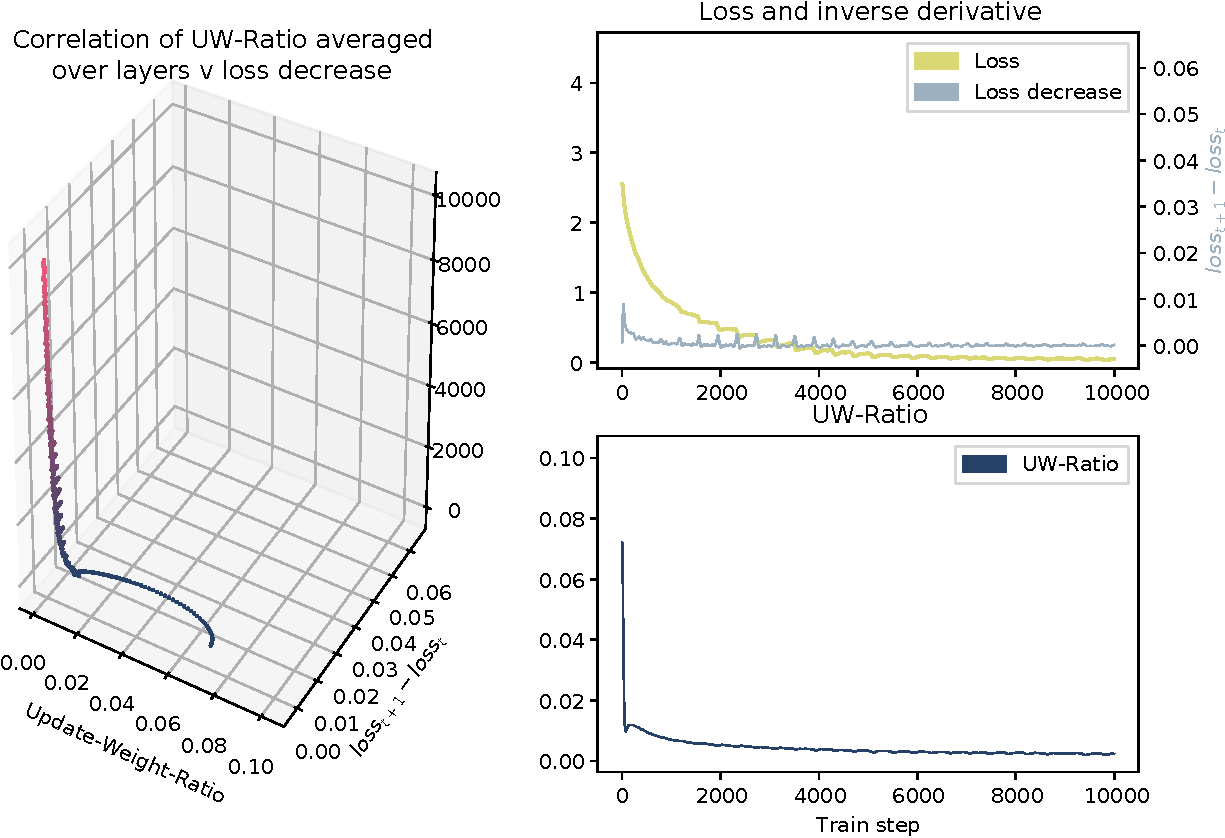
\includegraphics[width=\linewidth]{gfx/diagrams/experiments/ratio_loss_correlation/vgg_adam_001_0_10000.pdf}
        \caption{UW ratio experiment for VGG with Adam and learning rate $0.01$}
        \label{fig:ratio_loss_corr_vgg_adam_001}
    \end{subfigure}

    \begin{subfigure}{\textwidth}
        \centering
        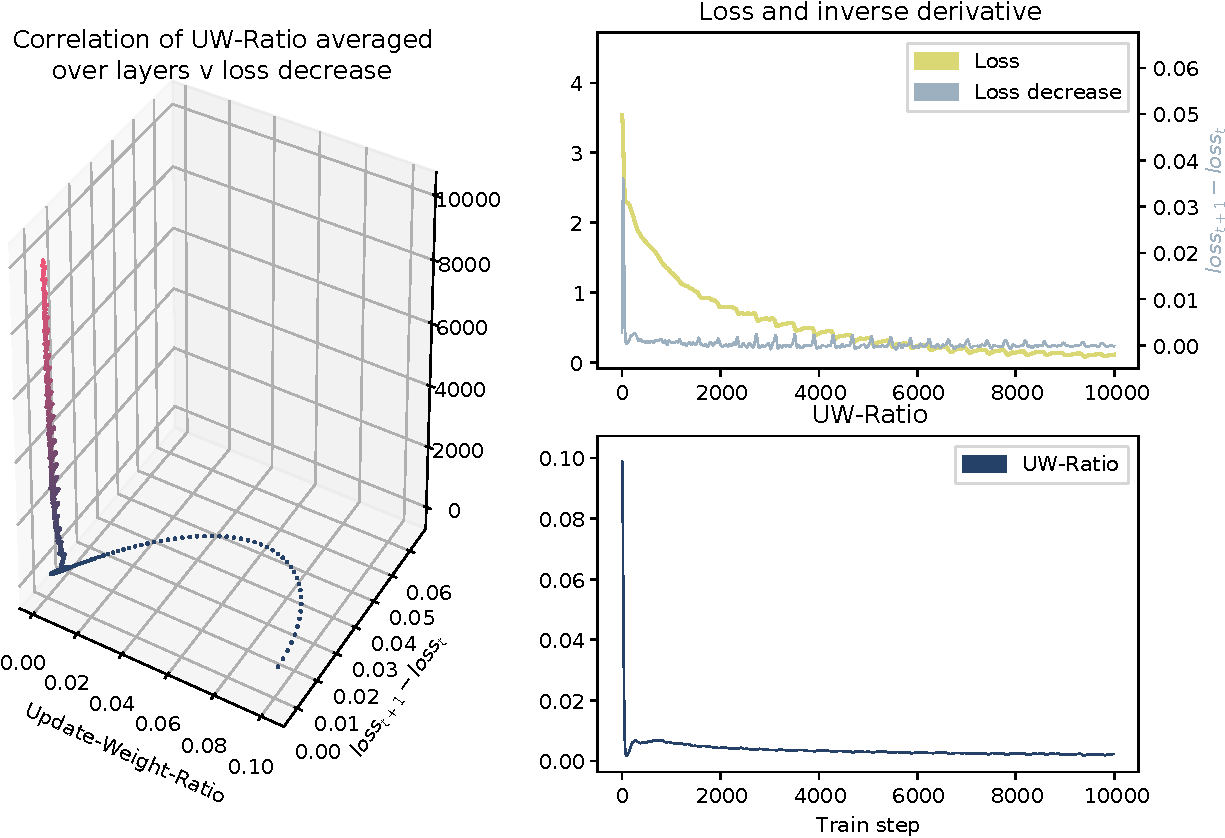
\includegraphics[width=\linewidth]{gfx/diagrams/experiments/ratio_loss_correlation/vgg_adam_005_0_10000.pdf}
        \caption{UW ratio experiment for VGG with Adam and learning rate $0.05$}
        \label{fig:ratio_loss_corr_vgg_adam_005}
    \end{subfigure}

    \begin{subfigure}{\textwidth}
        \centering
        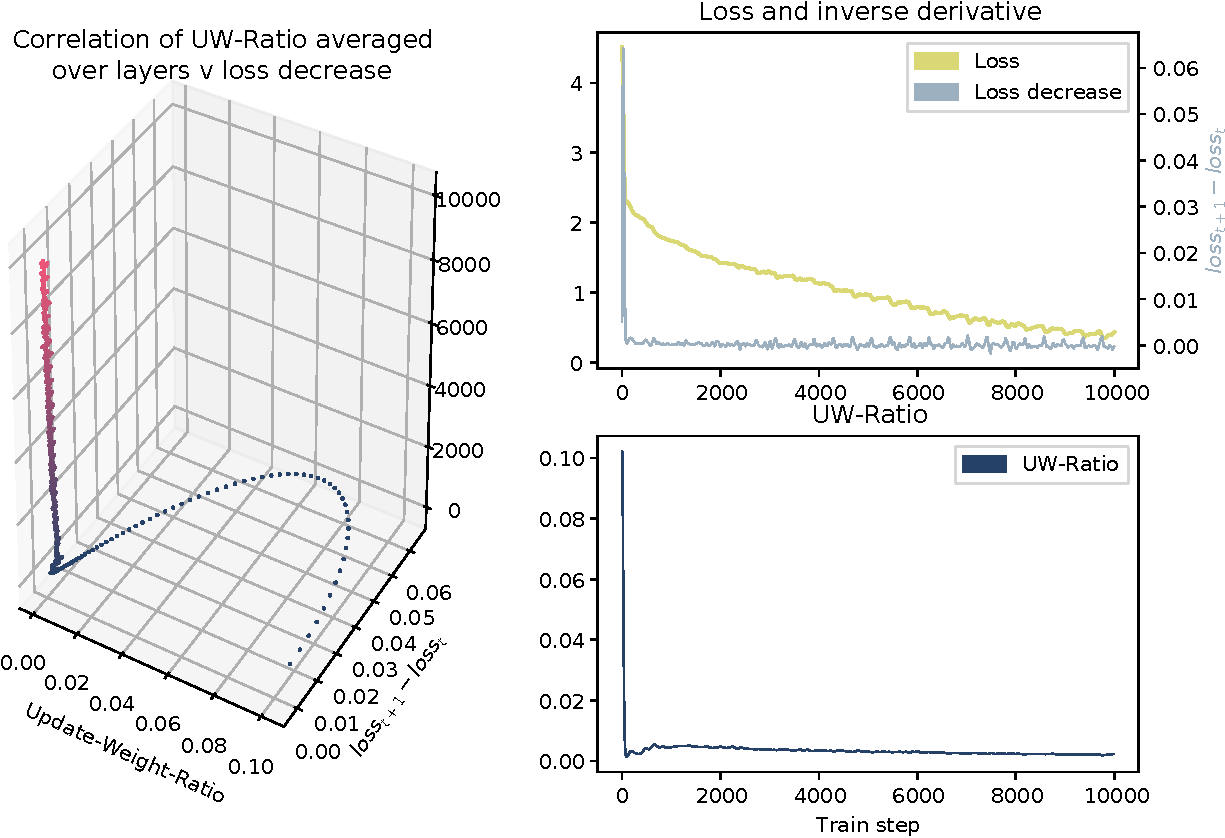
\includegraphics[width=\linewidth]{gfx/diagrams/experiments/ratio_loss_correlation/vgg_adam_01_0_10000.pdf}
        \caption{UW ratio experiment for VGG with Adam and learning rate $0.1$}
        \label{fig:ratio_loss_corr_vgg_adam_01}
    \end{subfigure}
\end{figure}

Remarkably, the qualitative behaviour is the opposite of SGD, which becomes visible
when omitting the first few hundred training steps. While for SGD (plots omitted
for brevity), higher learning rates lead to higher initial values in the UW
distribution, the opposite seems to hold for the adaptive optimizer. This can be
seen in
\cref{fig:ratio_loss_corr_vgg_adam_001_500,fig:ratio_loss_corr_vgg_adam_005_500,fig:ratio_loss_corr_vgg_adam_01_500}
where the first $500$ training steps are omitted to avoid squishing the
scatter plot because of the quickly decaying arcs in the beginning of training.
A possible explanation is that Adam uses estimates of the mean and variance of
gradients, and possibly overcorrects the learning rate.

\begin{figure}
    \begin{subfigure}{\textwidth}
        \centering
        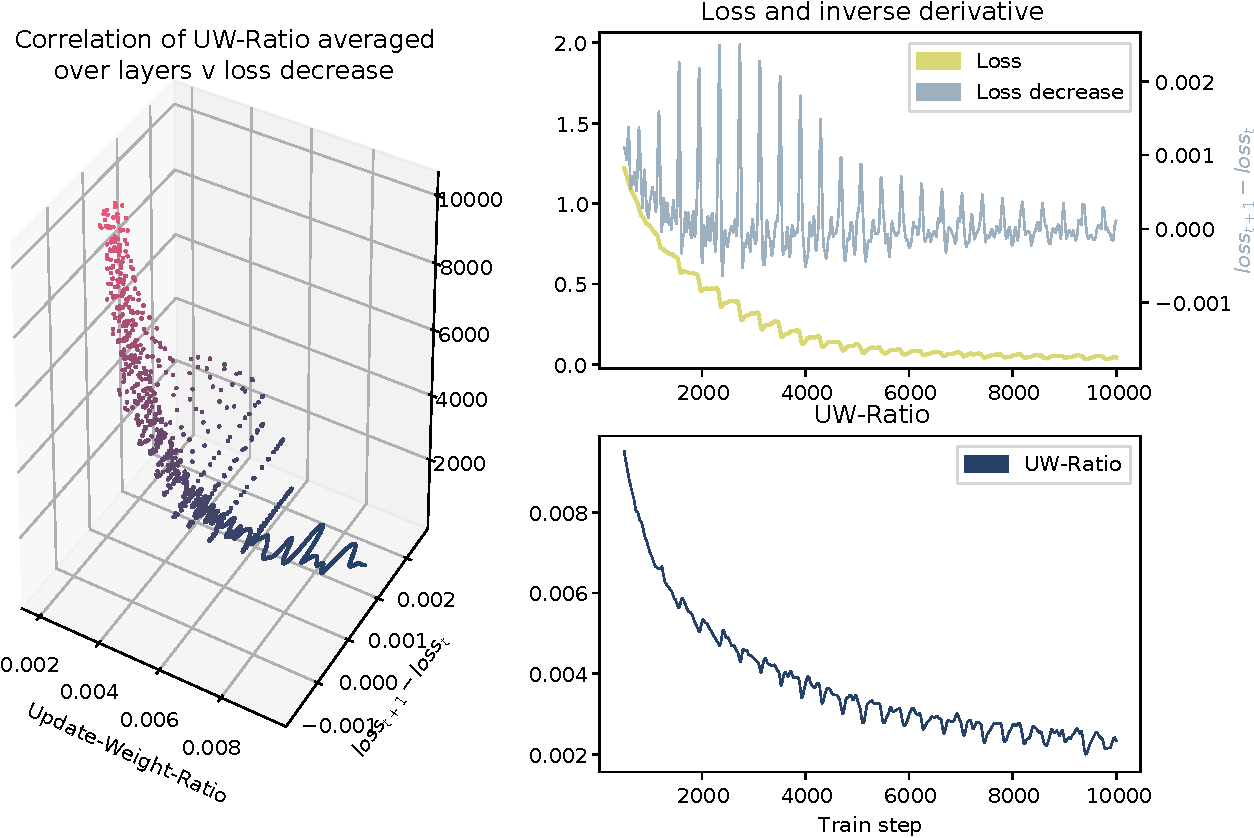
\includegraphics[width=\linewidth]{gfx/diagrams/experiments/ratio_loss_correlation/vgg_adam_001_500_10000.pdf}
        \caption{UW ratio experiment for VGG with Adam and learning rate $0.01$,
        beginning at step $500$}
        \label{fig:ratio_loss_corr_vgg_adam_001_500}
    \end{subfigure}

    \begin{subfigure}{\textwidth}
        \centering
        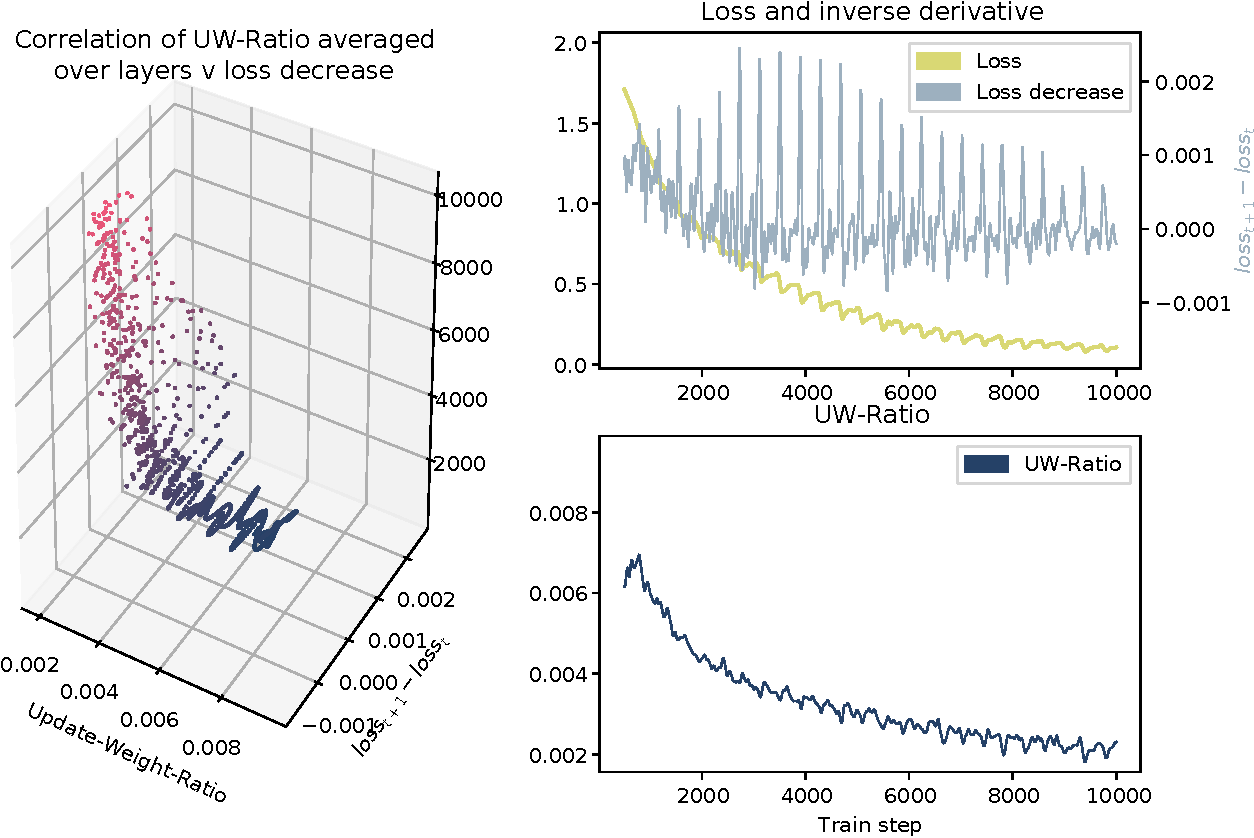
\includegraphics[width=\linewidth]{gfx/diagrams/experiments/ratio_loss_correlation/vgg_adam_005_500_10000.pdf}
        \caption{UW ratio experiment for VGG with Adam and learning rate $0.05$,
        beginning at step $500$}
        \label{fig:ratio_loss_corr_vgg_adam_005_500}
    \end{subfigure}

    \begin{subfigure}{\textwidth}
        \centering
        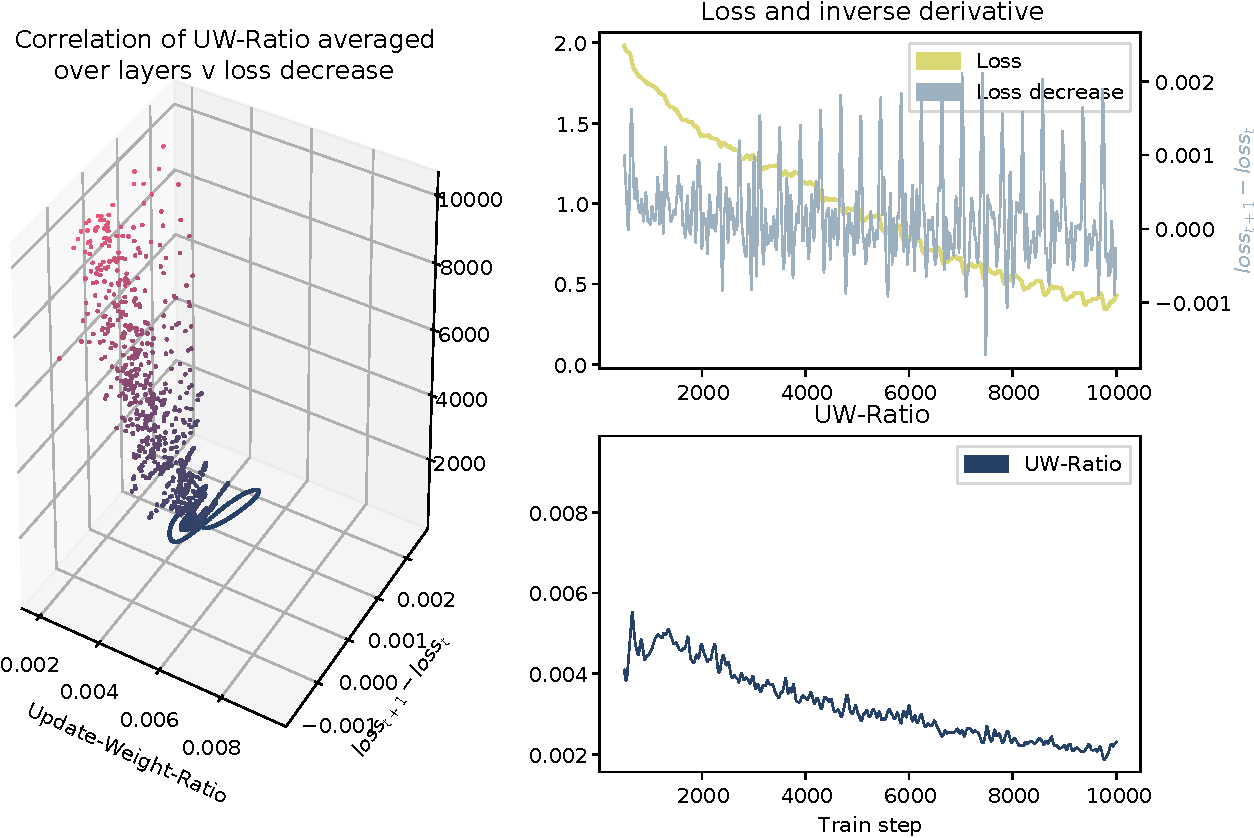
\includegraphics[width=\linewidth]{gfx/diagrams/experiments/ratio_loss_correlation/vgg_adam_01_500_10000.pdf}
        \caption{UW ratio experiment for VGG with Adam and learning rate $0.1$,
        beginning at step $500$}
        \label{fig:ratio_loss_corr_vgg_adam_01_500}
    \end{subfigure}
\end{figure}

\subsubsection{Other Architectures}

Several analyses were conducted on the data, but not displayed here due to
inconclusive results. \textcolor{red}{Put plots into appendix to beef up thesis!}
The experiments were run on the AlexNetMini architecture as well, without
results, as the network does not converge within $75$ epochs.
The same experiment on the ResNet18 architecture exhibited the same qualitative
behaviour as the VGG network, except for a larger variance in loss decreases for
a given ratio value. Slicing the training into pieces and graphing every slice
of $5,000$ training steps separately reveals nothing beyond a decrease in
absolute value of ratio and loss, which is expected. Any correlations between
the two quantities do not change after the initial few steps.

\subsubsection{Summary}

The results from all these experiments do not demonstrate that a ratio value
of $0.001$ is any more significant than others. While it is intuitive that the loss
can only decrease significantly if the weights change accordingly (unless the
loss surface is extremely rough), we find no particular insights as to what
ratio is appropriate for any given point in training.

\subsubsection{Fixing The Learning Rate for Karpathy's Constant}

We now want to check how the UW ratio relates to the loss when we attempt to
artificially fix the ratio value to a target of $0.001$. Since the updates to the
weights in vanilla SGD (see \cref{sec:review_stochastic_gradient_descent}) are a
function of the learning rate and the gradient magnitude, this could be done in
one of two ways:
\begin{enumerate}
    \item Scale the gradients with the constant learning rate in mind
    \item Set the learning rate according to the ratio-adaptive schedule from
        \cref{sub:ratio_adaptive_learning_rate_scheduling}
\end{enumerate}

Using the ratio-adaptive schedule results in the behaviour shown in
\cref{fig:ratio_loss_corr_vgg_sgd_0001_adaptive,fig:ratio_loss_corr_vgg_sgd_001_adaptive,fig:ratio_loss_corr_vgg_sgd_01_adaptive}.
In contrast to previous experiments, we also have a configuration with $0.001$
learning rate, dropping the $0.05$ value. We also plot the learning rate caused
by the scheduling over the UW ratio.

Note that for this set of plots, the axis limits are different. This serves to
illustrate that the qualitative behaviour is identical for all learning rates
(ignoring the fast arc at the beginning for $\text{lr}=0.1$). The learning rate
trajectories are very similar; the learning rate rises as the UW ratio
decreases. The primary insight from these experiments is that the empirical UW ratio is
not linearly related to the learning rate. Recall from
\cref{sec:review_stochastic_gradient_descent} that the weight update is given by
\begin{align}
    \eta \nabla_{\boldsymbol\theta}J,
\end{align}
so it is a linear function of the learning rate and the gradient magnitude. We
would therefore expect that a tenfold reduction in learning rate would result in
an equal reduction in the UW ratio. However, the difference is not quite as
pronounced in reality. Considering
\cref{fig:ratio_loss_corr_vgg_sgd_001_adaptive} and
\cref{fig:ratio_loss_corr_vgg_sgd_01_adaptive} we see the learning rate
differing by a factor of $\sim{}5$, whereas the UW ratios only differ by a factor of
$\sim{}2$. The cleft between reality and expectation is even more pronounced for
learning rates $0.001$ and $0.1$. This hints at a qualitative difference between
the paths through parameter space taken by higher vs. lower learning rates. If
we assume the directions are mostly the same, we would also expect the higher
learning rate to traverse them quicker (entailing a larger weight change and
thus a higher UW ratio, but possibly suffering from the usual problems of
too-high learning rate). If instead the path taken by the higher learning rate
is actually less steep than the one taken by the smaller rate, we could observe
the phenomenon documented here.

\begin{figure}
    \begin{subfigure}{\textwidth}
        \centering
        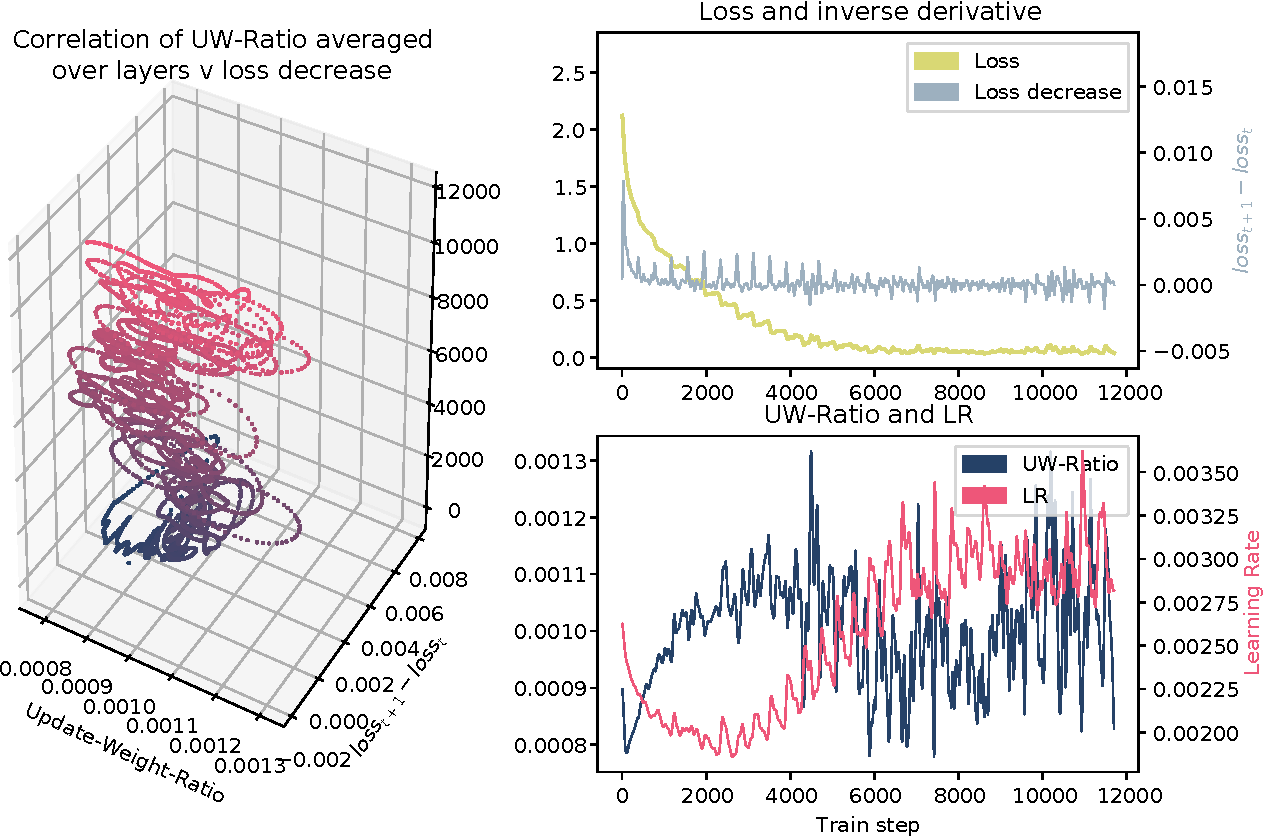
\includegraphics[width=\linewidth]{gfx/diagrams/experiments/ratio_loss_correlation/vgg_sgd_0001_0_11700_ratio_schedule.pdf}
        \caption{UW ratio experiment for VGG with SGD and adaptive learning rate
            from $0.001$}
        \label{fig:ratio_loss_corr_vgg_sgd_0001_adaptive}
    \end{subfigure}

    \begin{subfigure}{\textwidth}
        \centering
        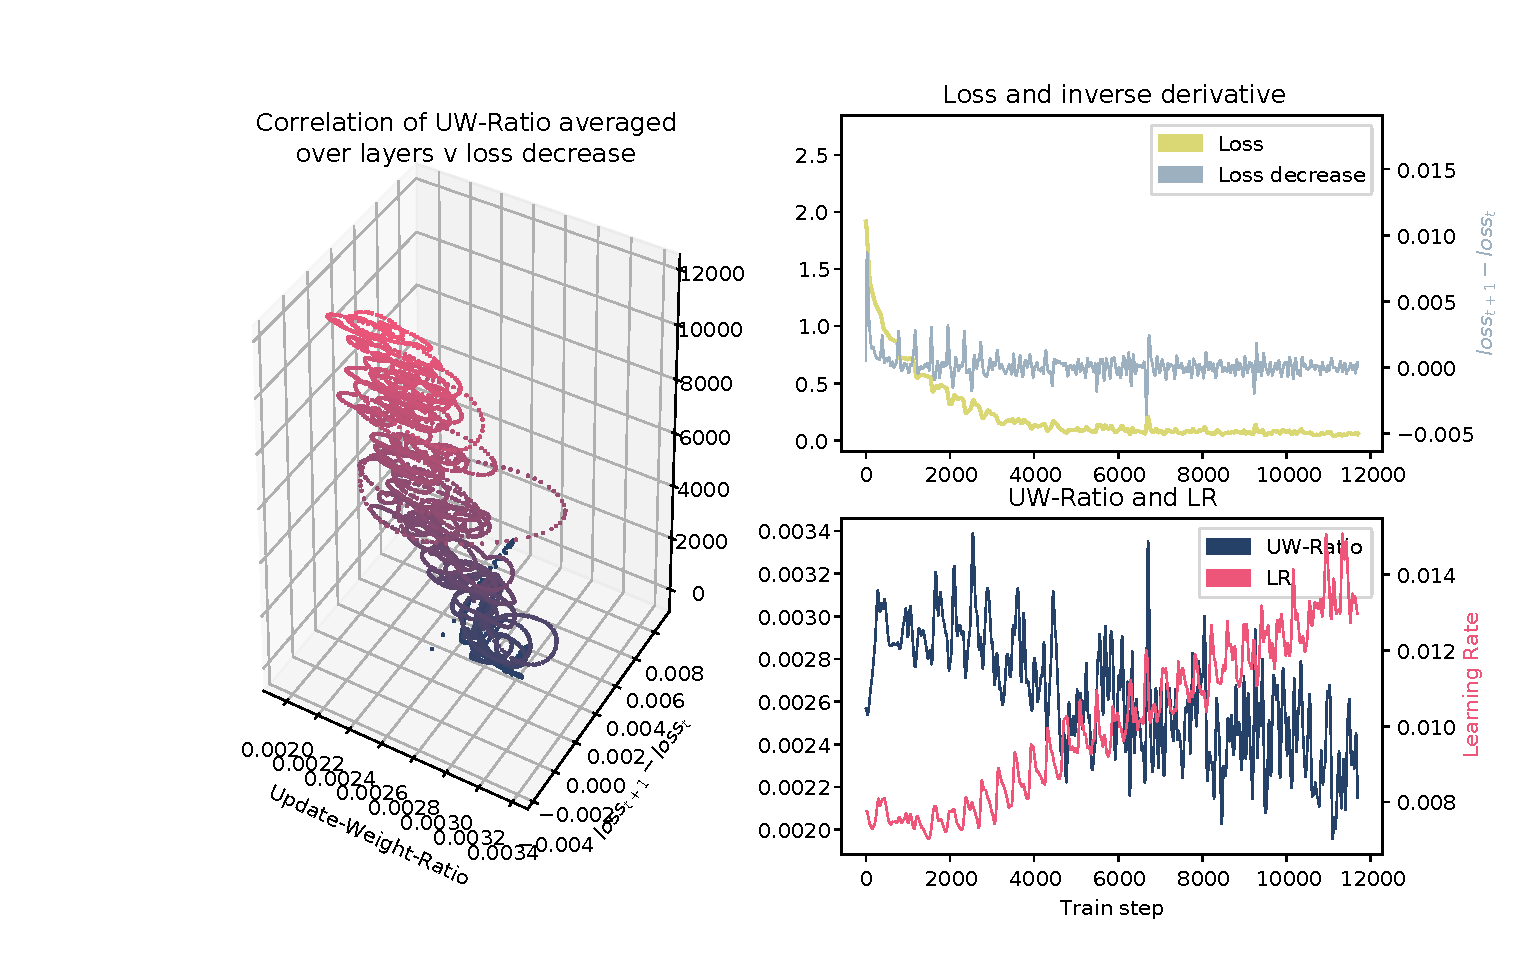
\includegraphics[width=\linewidth]{gfx/diagrams/experiments/ratio_loss_correlation/vgg_sgd_001_0_11700_ratio_schedule.pdf}
        \caption{UW ratio experiment for VGG with SGD and adaptive learning rate
            from $0.01$}
        \label{fig:ratio_loss_corr_vgg_sgd_001_adaptive}
    \end{subfigure}

    %% leave this as only 3 fit on one page
    % \begin{subfigure}{\textwidth}
    %     \centering
    %     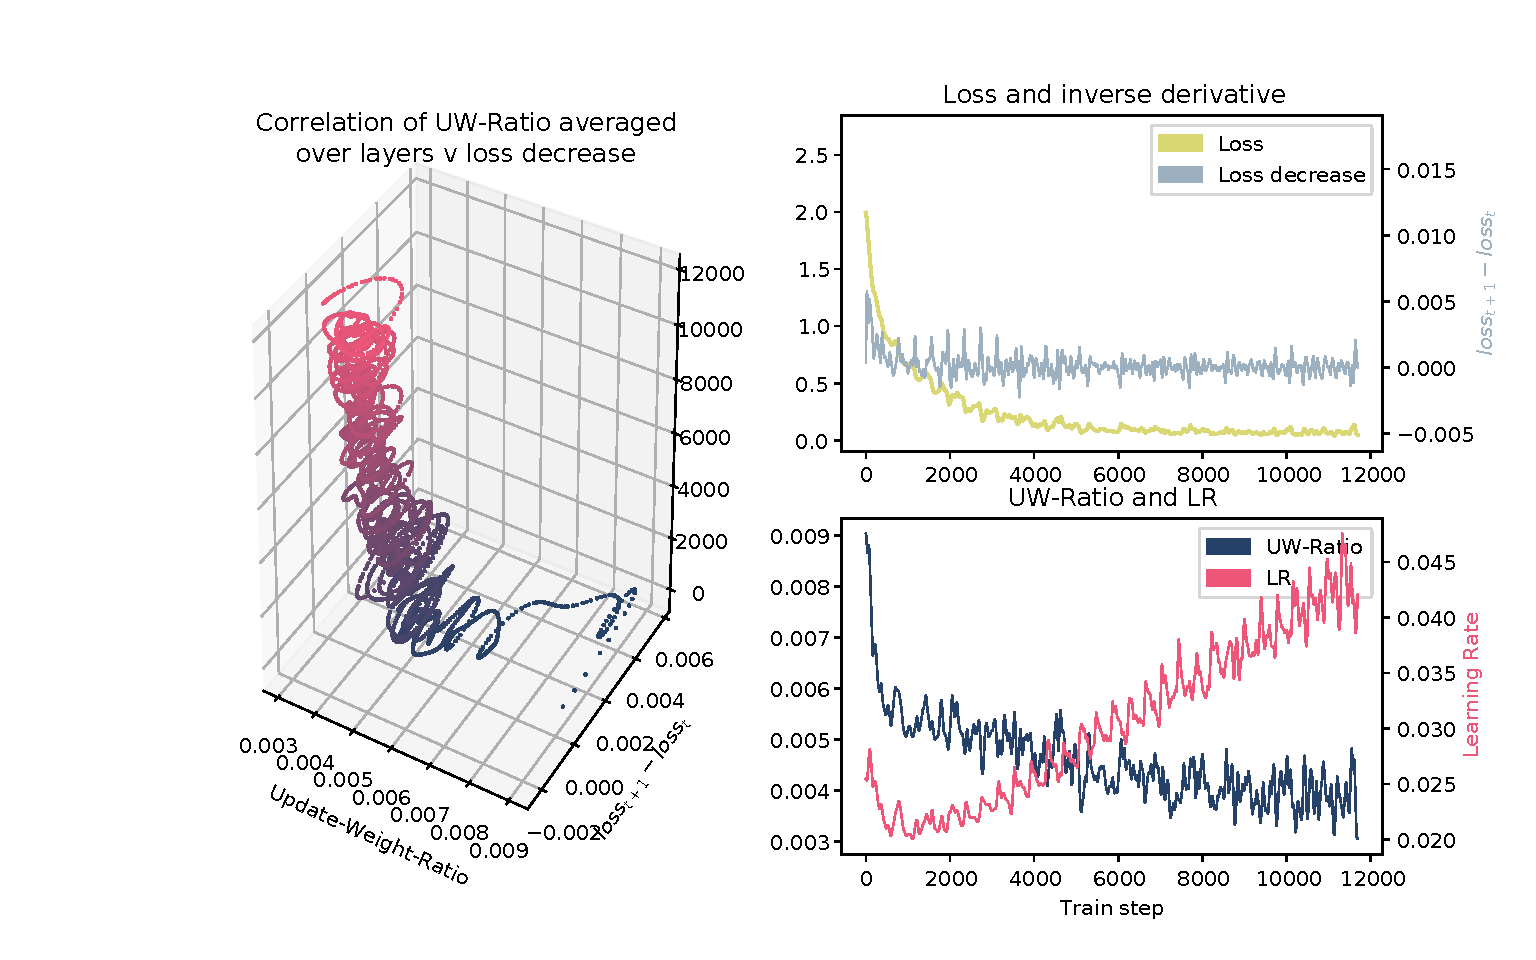
\includegraphics[width=\linewidth]{gfx/diagrams/experiments/ratio_loss_correlation/vgg_sgd_005_0_11700_ratio_schedule.pdf}
    %     \caption{UW ratio experiment for VGG with SGD and learning rate adaptive
    %         from $0.05$}
    %     \label{fig:ratio_loss_corr_vgg_sgd_005_adaptive}
    % \end{subfigure}

    \begin{subfigure}{\textwidth}
        \centering
        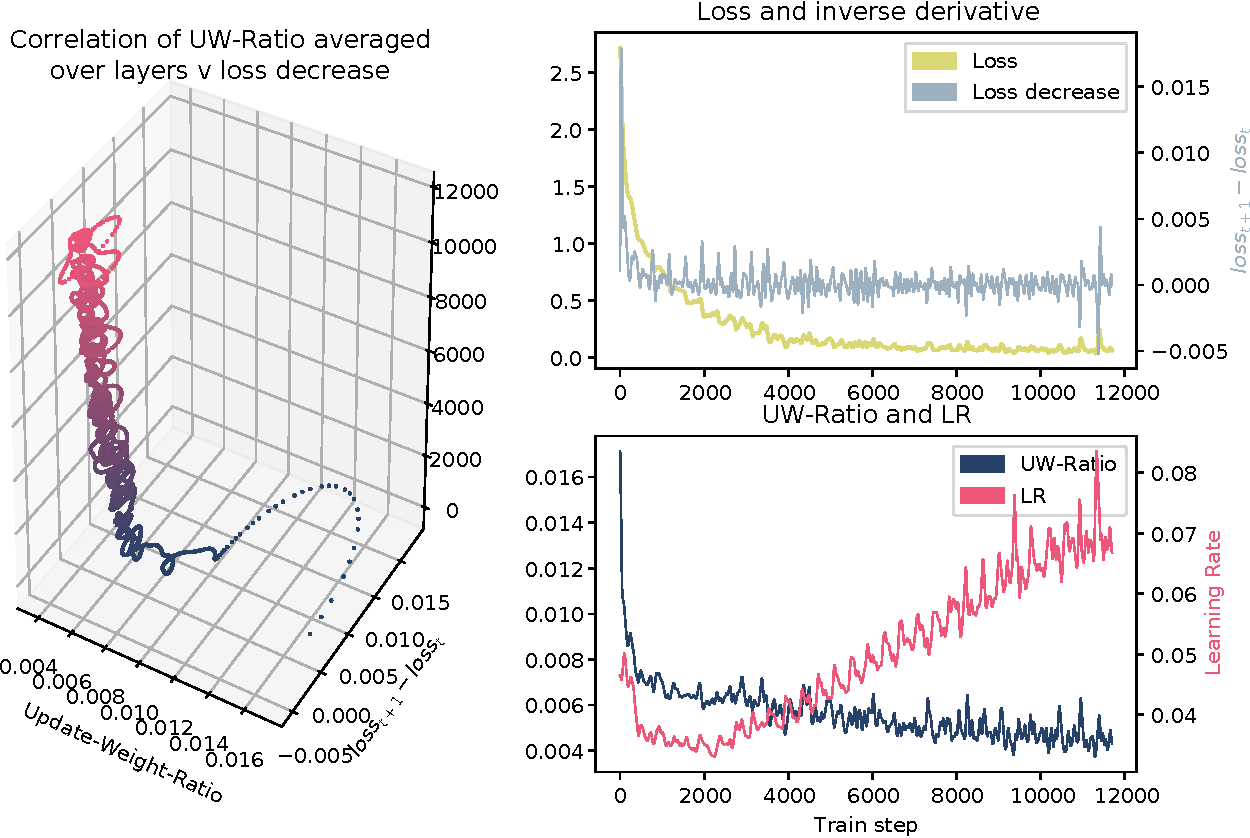
\includegraphics[width=\linewidth]{gfx/diagrams/experiments/ratio_loss_correlation/vgg_sgd_01_0_11700_ratio_schedule.pdf}
        \caption{UW ratio experiment for VGG with SGD and adaptive learning rate
            from $0.1$}
        \label{fig:ratio_loss_corr_vgg_sgd_01_adaptive}
    \end{subfigure}
\end{figure}

\subsubsection{Summary}

The two experiments with a dynamic learning rate schedule based on the average
ratio of updates and parameters do not yield any definitive insights into
whether any one value should be considered a target metric. It was obvious from
the beginning that as the loss curve approaches its asymptote, the change to the
weights needs to decrease, and indeed this has been demonstrated clearly. It is
not clear at this point whether the UW ratio provides additional information
over other metrics such as the loss curve itself or the norm of the gradients,
but the experiments in influencing the ratio have proven that there is no
obvious dependency between them---problems can still be learned with a smooth
loss decrease even when influencing the UW ratio via learning rate scheduling.

However, more work would be necessary to check whether a moving target could
help optimisation. We have seen througout this section that  when learning works
well, the ratio decays similarly to a an exponential, which opens the
possibility for scheduling the learning rate with some decay function and a base
value (such as $10^{-3}$).  While this may not aid convergence in cases that are
well-behaved, it could move models out of areas they would otherwise spend too
much time in, or reduce parameter oscillations in the face of highly noisy loss
surfaces.

With the help of \texttt{ikkuna}, one could easily implement a ratio-based
learning rate schedule with e.g. exponential decay built-in and test its
performance on a wide range of models and datasets.

\section{Measuring Layer Saturation for Early Stopping}%
\label{sec:detecting_layer_saturation}

As a last study, we want to investigate an approach for automatically detecting
when a good time for stopping parameter updates for a layer comes around. In
other words, we are concerned with \emph{freeze training} in which we freeze
layers according to some criterion, thus saving computation time during the
backward pass. This only makes sense, however, if we do not lose validation
accuracy this way.

The term ``early stopping'' generally refers to halting training completely
based on some criterion, often derived from the current training and validation
accuracy of the model. It is used to avoid overfitting the model to the dataset
by iterating over the dataset too often, until the model essentially memorises
the data. In contrast, we use the term for the more fine-grained approach to
freezing individual layers at points during training.

\subsection{Background}%
\label{sub:saturation-background}

Recently, the idea of saving computation by progressively freezing layers has
been put forth by \citet{brock2017freezeout}. They use individual decaying
learning rates for each layer so that the rate drops to zero at some point in
training. Different schedules for annealing the learning rates are investigated
and tradeoffs between validation accuracy and computational savings are
reported. The results are that up to $20\%$ of total training time can be saved
with less than $3\%$ loss in accuracy for DenseNets \citep{huang2017densely} and
ResNets \citep{he2016deep} while a VGG variant does not show the same promise.
\citeauthor{brock2017freezeout} hypothesise that skip-connections play an
important role for enabling a good time-accuracy tradeoff, as they are not
present in the fully convolutional VGG model.

The approach investigated in this section draws inspiration from
\citep{raghu2017svcca}, where a similarity measure between the representations
learned by different layers in the same or different neural networks is defined
an evaluated. \citeauthor{raghu2017svcca}'s experiments show that layers
generally converge bottom-up by computing their similarity between points during
training and the final state. This insight motivates freezing each layer at a
percentage of training time, which is a simpler heuristic than the one proposed
by \citeauthor{brock2017freezeout}. Freezing layer $i$ at time
$\frac{i}{n_\text{layers}} \cdot n_\text{iterations}$ even leads to small improvements
in validation accuracy.

After introducing the method of Singular Vector Canonical Correlation Analysis
(SVCCA) used by \citeauthor{raghu2017svcca}, we will apply it as a metric for
measuring layer saturation or convergence by computing the similarity between
each layer and itself after the previous epoch. We will compare the usefulness
of this metric in informing a freezing schedule with the aforementioned fixed
schedule.

\subsection{Singular Vector Canonical Correlation Analysis}%
\label{sub:singular_vector_canonical_correlation_analysis}

\citet{raghu2017svcca} propose a measure for comparing the similarity of
``representations'' learned by layers in neural networks. In this context, the
representation is defined as the set of activations of a layer's neuron over
some dataset $D$ (usually a subset of the training data). Formally, a layer is given
as the set of activation vectors of its units, each of which has $n := |D|$ individual
activations.
\begin{align}
    L_k & :=  \left\{ (a_{k,i}(\mathbf{x}_0), \ldots, a_{k,i}(\mathbf{x}_{n-1})) \mid i \in [0,n_\text{units})\right\}
\end{align}
A layer's representation can hence be thought of as a subspace of
$\mathcal{R}^n$. However, this primitive concept of a layers learned
representation has several problems
\begin{itemize}
    \item It is not clear whether all directions in the subspace are equally
        important. Indeed, as the number of parameters often exceeds the number
        of training examples, most networks are mathematically overparameterised
        and thus redundant by default (in the absence of regularisation).
        Previous work (e.g.
        \citet{lecun1990optimal,srinivas2015data,molchanov2016pruning} report
        significant computational savings through removing unnecessary units).
        Using the representations as they are would therefore incorporate many
        noisy, unstable and unimportant parameters.
    \item Since the dimension spanned by the activation vectors can be different
        between layers---as different numbers of units enable more or fewer
        linearly independent basis vectors---layers of different size could not
        be straightforwardly compared e.g. by finding an transformation from one
        space to the other, but it is desirable to compare representations
        between layers and even networks
\end{itemize}

The first issue is addressed by reducing the dimensionality of $\Span{L_k}$ by
principal component analysis.

\begin{align}
    \label{eq:cov}
    \intertext{First we obtain the data matrix for a layer}
    L_k   & = (a_{k,i,0}, a_{k,i,1}, \ldots, a_{k,i,n-1})^T  \in \mathcal{R}^{n_\text{units} \times n} \\
        & =
            \begin{bmatrix}
                a_{k,0}(\mathbf{x}_0) & \ldots & a_{k,0}(\mathbf{x}_{n-1}) \\
                \vdots          & \ddots & \vdots \\
                a_{k,n_\text{units}-1}(\mathbf{x}_0) & \ldots & a_{k,n_\text{units}-1}(\mathbf{x}_{n-1})
            \end{bmatrix} \\
    \intertext{We then get a matrix whose rows are identical---the mean over the first dimension}
    M_k & = (1, \ldots, 1)^T \cdot \frac{1}{n}\sum_{i=0}^{n-1} L_k(i,:)
    \intertext{We can then compute the centered covariance matrix of the data}
    C   & = (L_k - M_k)^T \cdot (L_k - M_k)
    \intertext{Diagonalising this matrix through SVD yields}
    C   & = U \Sigma V
\end{align}
with $\Sigma$ containing the singular values and $U\Sigma$ being
the transformation matrix to the lower-dimensional space (according to
number of singular values and vectors chosen).

In doing so, a new
lower-dimensional basis of orthogonal singular vectors is found, a projection
to which preserves the most possible variance in the data. The dimensionality
can be selected by considering that the magnitude of the singular values is
proportional to the amount of variance in the data that is captured by the
associated singular direction. A number of singular directions is selected so
as to capture $99\%$ of the variance of the data. After projecting the data onto
the thusly determined principal components, low-variance directions (which are
neurons) are removed.

PCA is performed on both layers to compare, in our case, the same layer at
different points in training. The dimensionality-reduced layer representation is
then processed with canonical correlation analysis (CCA).  Given vectors of
random variables $X=(X_0, \ldots, X_m)$, $Y=(Y_0, \ldots, Y_l)$, CCA finds
linear combinations $a$, $b$ of both sets so that the correlation $\rho =
corr(aX^T, bY^T )$ between the transformed random variables is maximised. When
the first transformation is found, a second one can be computed under the
constraint that the resulting transformed random variables be uncorrelated with
the first pair of transformed variables, then the third and so forth. The result
of CCA is a set of $\min\{m,l\}$ correlation coefficients which can be distilled
into a similarity measure for learned representations, e.g. by taking the
average. The result is a correlation between sets of neuronal activations that
is invariant to linear transformations and is not influenced by low-variance or
zero activations. The motivation for using this similarity as opposed to simply
correlating activations between two time steps is that the CCA correlation
allows a layer to change in a linear way between two steps, but we are not
interested in how a layer's output distribution is located in space exactly, but
what kind of representation it has learned. This additional invariant behaviour
could be more robust to noisy and ultimately pointless changes in a layer's
weights which we would otherwise conclude from that the layer has changed
significantly while it effectively has not.

As a side-effect of CCA, layers of different size can be related, since the
input vectors of random variables need not be of the same length. This property
is important for comparing different layers and architectures, but immaterial
for our experiments.

Todo: Elaborate on difference between linear and conv layers

\subsection{Implementation of SVCCA}%
\label{sub:implementation_of_svcca}

\citeauthor{raghu2017svcca} released the code used for the
publication\footnote{\url{https://github.com/google/svcca}} under an Apache 2.0
open source license. The implementation uses NumPy and therefore only runs on
the CPU. For this work, a fork was created which enables the computations to run
transparently on NumPy, PyTorch or CuPy\footnote{CuPy is a GPU-enabled library
implementing a subset of the NumPy API; it is developed for the deep learning
framework Chainer.}\footnote{The library can be found at
\url{https://github.com/themightyoarfish/svcca-gpu}}, so  that expensive memory
transfers between CPU and GPU can be avoided. Additionally, many of the matrix
operations can benefit from GPU acceleration. Making the computations fast
enough to compute the similarity often enough on each layer is essential for
using it as an on-line metric.

An issue was discovered during benchmarking the CPU and GPU versions against one
another: The covariance matrix computed on the activations for many layers
turned out to be highly ill-conditioned when using PyTorch for computing it,
seemingly due to small numerical deviations. While almost identical to the human
observer, the small differences between the covariances often leads to a
convergence failure of the SVD routine used in PyTorch. Since it is not unlikely
that different units in a layer exhibit the same response to data points --
especially in the beginning of training---some redundancy in the activations
can be expected and repeated datapoints lead to ill-conditioned covariance
matrix. For this reason \citeauthor{raghu2017svcca} implement a robust version
of the similarity computation in which noise is progressively added to the
activations before the computations until the procedure converges successfully.
Other potential workarounds for ill-conditioned covariances include
\begin{itemize}
    \item Adding a small constant to the diagnoal of the covariance matrix (this
        is known as \emph{nugget regularisation})
    \item Adjusting the threshold parameter generally used in SVD algorithms to
        cut off singular values close to zero
\end{itemize}
The efficacy of these parameters would need extensive evaluation.

This solution notwithstanding, it turned out
that the \texttt{torch.mean()} function behaves slightly differently from the
the NumPy equivalent, possibly losing precision somewhere, which changes the
covariances (see \cref{eq:cov}).  The entries of the covariance matrices are
often smaller than $0.1$, while maximal differences between NumPy and PyTorch
computations reach values of $0.05$, which is very large in relation to the
values.
Floating point arithmetic, at least in the IEEE 754 specification generally used
in computing, is neither completely commutative nor associative, so the order in
which operations are performed can impact the result, so this behaviour is
expected\footnote{\url{https://github.com/pytorch/pytorch/issues/16569}}. This
does not usually lead to problems, but in this use case appears to be highly
dangerous. It is unclear in which circumstances the problem arises exactly and a
more thorough investigation would be necessary.

For this reason, the experiments
performed here use NumPy for computing the SVCCA metric. This incurs high data
transfer overhead, but is more stable and sufficient to answer the question of whether the
metric can be useful at all. An investigation of the limitations of the GPU
impelementation is left for future work.


\subsection{Experiments}%
\label{sub:saturation-experiments}

The hypothesis to be tested in this seciton is whether the similarity of a layer
to itself at previous point in training can be used as a heuristic for
determining when to stop training the layer, thus saving all gradient
computation for this layer. For this purpose a dedicated subscriber is
implemented which periodically feeds a dataset through the network, recording
all activations and then computing the SVCCA similarity with the current
activations and the ones recorded from the previous time step. The subscriber is
shown in \cref{lst:svcca_sub}.

\begin{lstlisting}[label={lst:svcca_sub},
caption={SVCCA Subscriber}]
class SVCCASubscriber(PlotSubscriber):

  def __init__(self, dataset_meta, n, forward_fn, freeze_at=10,
               message_bus=get_default_bus(), tag='default', subsample=1,
               ylims=None, backend='tb'):

    # unfortunately, we need access to the model for this subscriber in
    # order to initiate evaluation on the dataset
    self._forward_fn     = forward_fn
    self._previous_acts  = dict()
    self._current_acts   = dict()

    # get some random subset of the data
    indices              = np.random.randint(0, dataset_meta.size,
                                             size=n)
    dataset              = Subset(dataset_meta.dataset, indices)
    self._loader         = DataLoader(dataset, batch_size=n,
                                      shuffle=False,
                                      pin_memory=True)
    # cache input tensors so we don't repeatedly deserialize and copy
    self._input_cache    = []

    # similarity threshold for when to freeze layer
    self._freeze_at      = freeze_at
    self._ignore_modules = set()

    # subscribe 'batch_finished' message and also 'activations' with a
    # certain tag chosen by this subscriber to identify messages which come up
    # because it called forward() itself
    subscription1 = Subscription(self, ['batch_finished'], tag=tag, subsample=subsample)
    subscription2 = Subscription(self, ['activations'], tag='svcca_testing',
                                 subsample=1)

    # ... call super() and announce publications

  # these methods can be overriden by subclasses that implement more complex
  # forward propagations such as doing it in batches if the entire data set
  # can't be pushed through at once
  def _module_complete_previous(self, module):
    '''Check if activations for module are completely buffered from the previous step.'''
    return module in self._previous_acts

  def _module_complete_current(self, module):
    '''Check if activations for module are completely buffered from the current step.'''
    return module in self._current_acts

  def _record_activations_previous(self, module, data):
    '''Record activations into the ``previous`` buffer'''
    self._previous_acts[module] = data

  def _record_activations_current(self, module, data):
    '''Record activations into the ``current`` buffer'''
    self._current_acts[module] = data

  def _do_forward_pass(self):
    # cache inputs initially
    if not self._input_cache:
        loader = iter(self._loader)
    else:
        loader = iter(self._input_cache)

    # here we make use of the modified forward() function patched in the
    # Exporter class. It accepts additional params for controlling the tag
    # under which messages are published as a result of this call.
    for i, (X, labels) in enumerate(loader):
        X = X.cuda()
        if len(self._input_cache) < i + 1:
            self._input_cache.append((X, labels))
        self._forward_fn(X, should_train=False, tag='svcca_testing')

  def _compute_similarity(self, name):
    # now both current and previous acts are complete and we can compute

    previous_acts = self._previous_acts.pop(name)
    current_acts = self._current_acts.pop(name)

    # current acts are now previous ones
    self._previous_acts[name] = current_acts

    # convolutional filters need to be reshaped to 2-d
    if previous_acts.ndimension() > 2:
      c = previous_acts.shape[1]  # channel dim
      previous_acts = previous_acts.permute([0, 2, 3, 1]).reshape(-1, c)

    if current_acts.ndimension() > 2:
      c = current_acts.shape[1]  # channel dim
      current_acts = current_acts.permute([0, 2, 3, 1]).reshape(-1, c)

    previous_acts = previous_acts.detach().cpu().numpy()
    current_acts = current_acts.detach().cpu().numpy()
    result_dict = svcca.cca_core.robust_cca_similarity(
                        previous_acts.T,
                        current_acts.T,
                        epsilon=1e-8,
                        threshold=0.98,
                        verbose=False,
                        compute_dirns=False,
                        rescale=True)
    return result_dict['mean'][0]

  def _freeze_module(self, module):
    print(f'Freezing {module}')
    freeze_module(module)
    self._ignore_modules.add(module)

    # clear any orphaned data
    if module in self._previous_acts:
        self._previous_acts.pop(module)
    if module in self._current_acts:
        self._current_acts.pop(module)

  def compute(self, message):

    if message.tag == 'default' and message.kind == 'batch_finished':
      # this means we are not in a state where we initiated forward
      # passes.
      # This assumes that the subsample initialiser parameter is set so
      # that this does not happen after every batch (unless desired)
      self._do_forward_pass()

    elif message.tag == 'svcca_testing':
      # we are receiving activation messages as a result of out call to
      forward_fn()
      module, name = message.key

      if module in self._ignore_modules:
        # maybe already frozen
        return

      if not self._module_complete_previous(module):
        self._record_activations_previous(module, message.data)
      elif not self._module_complete_current(module):
        self._record_activations_current(module, message.data)

      if self._module_complete_current(module) and self._module_complete_previous(module):
        mean = self._compute_similarity(module)
        self._backend.add_data(name, mean, message.global_step)

        # ... publish to message bus

        if mean > self._freeze_at:
          self._freeze_module(module)
\end{lstlisting}

The \texttt{SVCCASubscriber} holds a dataset and listens for messages that a
batch has ended. At this point, it will interrupt the training by passing its
dataset through the network, and attaches a custom \texttt{tag} to the messages
resulting from this call. This allows it to identify activation messages
originating from the call. It would be more ergonomic to have the data returned
directly from the call to \texttt{forward()}, but since the only way PyTorch
offers for retrieving intermediate layers' activations and gradients is
callback-based, \texttt{ikkuna} does not provide a simpler way of doing this at
the time of writing.

The activation messages are buffered until activations for both the previous
time step and the current one have been received, at which point the similarity
can be computed and published to the backend and message bus.

Several hyperparameters need to be decided on, and some parameters for the
similarity routine were fixed for theses experiments.
\begin{itemize}
    \item The dataset on
        which to evaluate the similarity must be decided. Since we are not interested in
        absolute predictions but simply in neuronal responses of different layers for
        the same data, it does not really matter whether the data is from training or
        validation sets. Ideally, however, it should have a maximally uniform class
        distribution so as to engage all filters that have been learned up to this
        point. If the data distribution was highly skewed, it could mean that some
        neurons never respond for any dataset, thus providing no information and
        reducing the rank of the covariance matrix (since some variables---columns of
        the data matrix $L_k$---would be linearly related) even though with a better
        dataset we might have had a larger rank and hence a different SV decomposition.
    \item A similarity threshold at which we determine the layer doesn't change
        anymore must be found. This value should be determined through thorough
        experimentation (\texttt{ikkuna} can be used to evaluate different
        thresholds on a wide range of models), but the experiments here use
        correlation thresholds of $0.99$ and $0.995$.
    \item The time scale at which significant layer changes are expected needs
        to be selected. If one was to compare a layer to itself at the previous
        training batch, one would expect very little change and thus a high
        correlation, whereas changes between the start of an epoch and the end
        would be much more significant. The experiments use epochs as the
        resolution and thus compute the measure at the end of every epoch.
\end{itemize}
\begin{table}
    \centering
    \caption{Hyperparameters for the saturation experiment}
    \label{tbl:params-saturation}
    \begin{tabular}{ll}
        Parameter            & Value \\\hline\hline
        Optimiser            & Vanilla SGD \\\hline
        Epochs               & $30$ \\\hline
        Dataset              & CIFAR10 \\\hline
        Batch size           & $512$ \\\hline
        Datapoints for SVCCA & $500$ \\\hline
        Nugget constant      & $10^{-8}$ \\\hline
        Learning rates       & $0.01, 0.1, 0.5$
    \end{tabular}
\end{table}

The hyperparameters used in these experiment are listed in
\cref{tbl:params-saturation}.  The experiment was run on the small convolutional
architecture (\cref{fig:alexnetmini}) as well as the larger VGG model
(\cref{fig:vgg16}). The self-similarity for each layer was computed at the
beginning of each epoch. We select high learning rates has have been found
appropriate for standard gradient descent. The different learning rates are
split among \cref{fig:saturation_alexnet_vgg_sgd_001_similarity} ($\eta = 0.01$),
\cref{fig:saturation_alexnet_vgg_sgd_001_similarity} ($\eta = 0.1$) and
\cref{fig:saturation_alexnet_vgg_sgd_05_similarity} ($\eta = 0.5$). All graphs are averages
of several runs, noted in parantheses in the legend. For thresholds on the
self-similarity score we use $0.99$, $0.995$ and also report control runs
without layer freezing (denoted by ``never'' in the graphs) and the heuristic
from \citep{raghu2017svcca} (see \cref{sub:saturation-background}).

\subsubsection{Layer Convergence and Validation Accuracy}

Focusing on the accuracy graphs (upper row) shows that for both thresholds and
models, accuracy is not negatively impacted, testifying that layer freezing can
always be appropriate. Except for the largest learning rate on the smaller model
(\cref{fig:saturation_alexnet_vgg_sgd_05_similarity}), the self-similarity-based
schedule for freezin is also not worse than the fixed one. For the smaller
model, freezing layers even resulted in increases accuracy. One explanation for
this could be that the model is more prone to overfit than the VGG network,
despite its smaller size. In that case, freezing layers before they start to
memorise the data could prevent this from happening.  For the higher of the two
thresholds, improvents could only be observed for the smaller two learning
rates. In contrast, at a learning rate of $0.5$, waiting until a layer reaches
$0.995$ saturation seems to allow the model to overfit too much, while the lower
learning rates are not high enough to show this problem.

On the other hand, the VGG model does not benefit from layer freezes
performance-wise. It is possible the architecture is less prone to overfit, thus
deriving no benefit from regularising it through freezes, besides reducing
computational cost.

We can draw the preliminary conclusion that progressively freezing layers is not
detrimental to performance, but saves computation.

It is also interesting to look at how the self-similarity for a layer evolves
throughout training (bottom row of plots). The similarity graphs for VGG show
strikingly, that according to this metric, layers converge bottom-up, without
fail, which is in line with \citet{raghu2017svcca}'s findings. Freezing
according to this metric therefore always results in successive layers getting
frozen, not disconnected ones. It is remarkable that in all cases, the first
layer of convolutions is converged already after the first five epochs, often
needing no more than one. All other layers need substantially longer. This makes
sense as the lower layers often learn spatial filters which act as edge
detectors. These filters are useful for any input, so the specific class
distribution almost does not matter. Because of this, it is not surprising that
$50.000$ training (one epoch) examples are enough to learn these filters.

\begin{figure}
    \centering
    \caption{Layer convergence experiment with learning rate $0.01$}
    \label{fig:saturation_alexnet_vgg_sgd_001}
    \begin{subfigure}{\textwidth}
        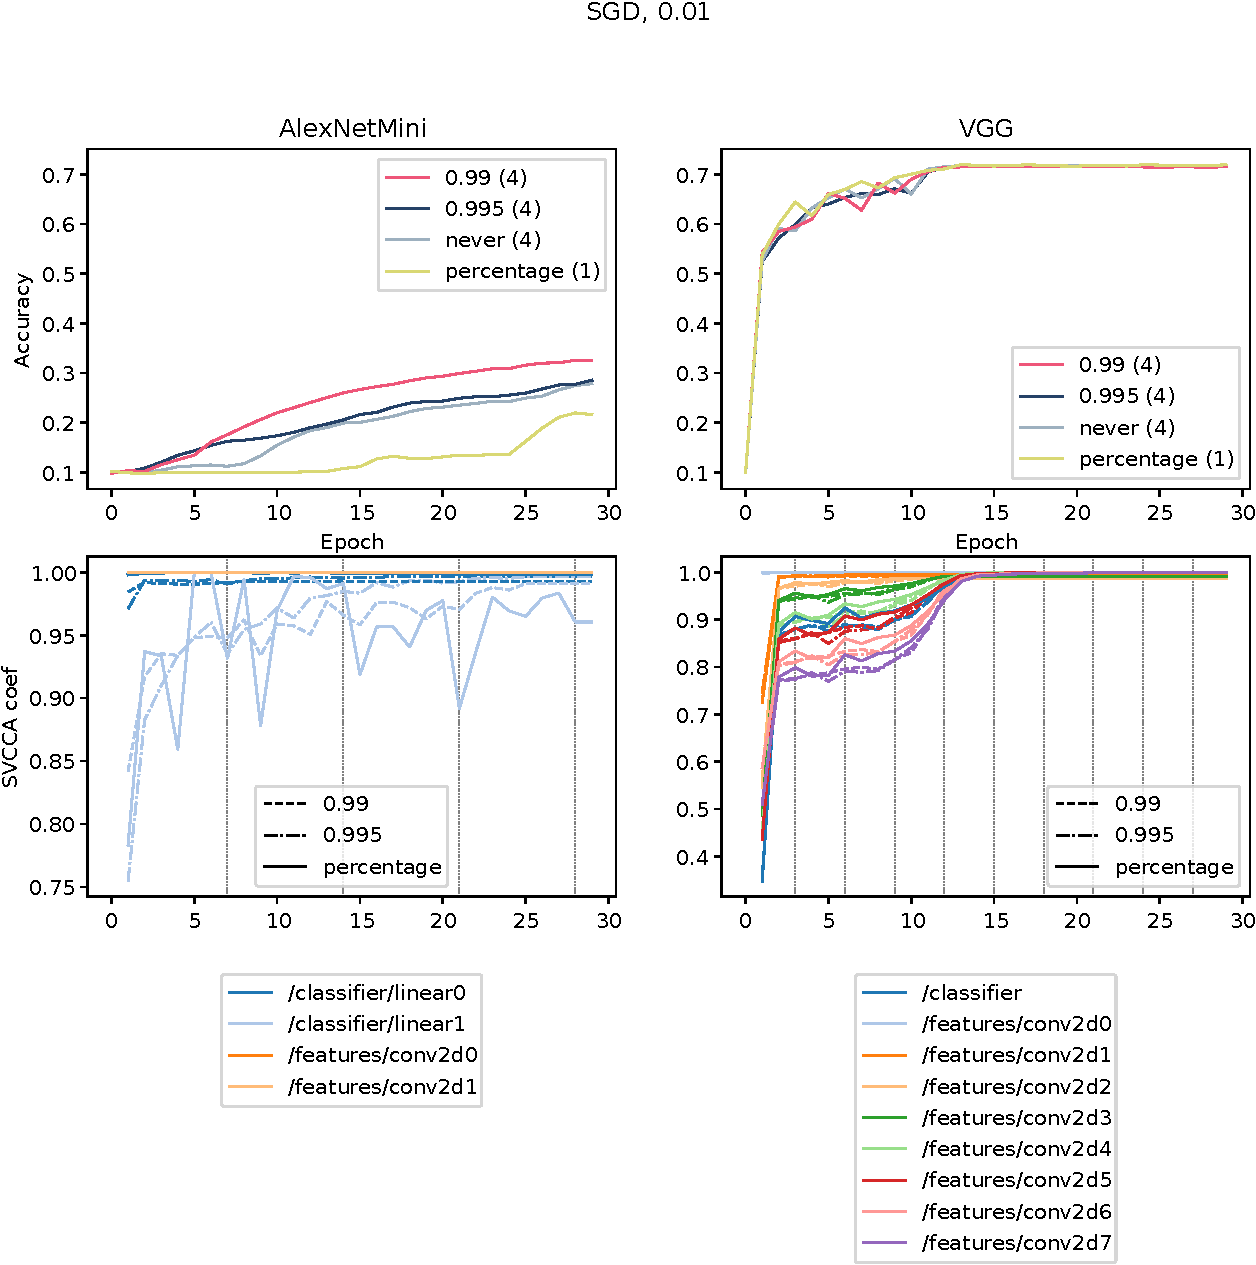
\includegraphics[width=\linewidth]{gfx/diagrams/experiments/saturation/acc_sim_alexnetmini_vgg_sgd_001.pdf}
        \caption{Accuracy and self-similarity for learning rate $0.01$}
        \label{fig:saturation_alexnet_vgg_sgd_001_similarity}
    \end{subfigure}

    \begin{subfigure}{\textwidth}
        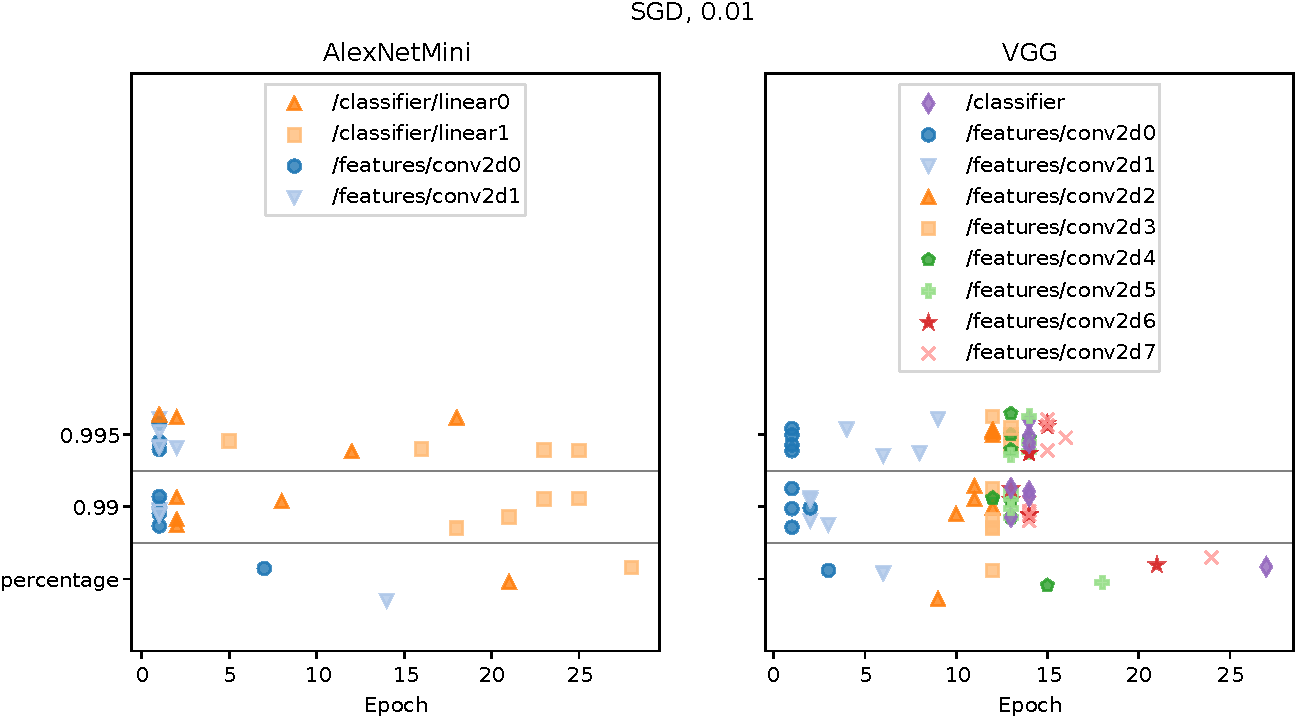
\includegraphics[width=\linewidth]{gfx/diagrams/experiments/saturation/convergence_alexnetmini_vgg_sgd_001.pdf}
        \caption{Freeze points for learning rate $0.01$}
        \label{fig:saturation_alexnet_vgg_sgd_001_convergence}
    \end{subfigure}
\end{figure}


\begin{figure}
    \centering
    \caption{Layer convergence experiment with learning rate $0.1$}
    \label{fig:saturation_alexnet_vgg_sgd_01}
    \begin{subfigure}{\textwidth}
        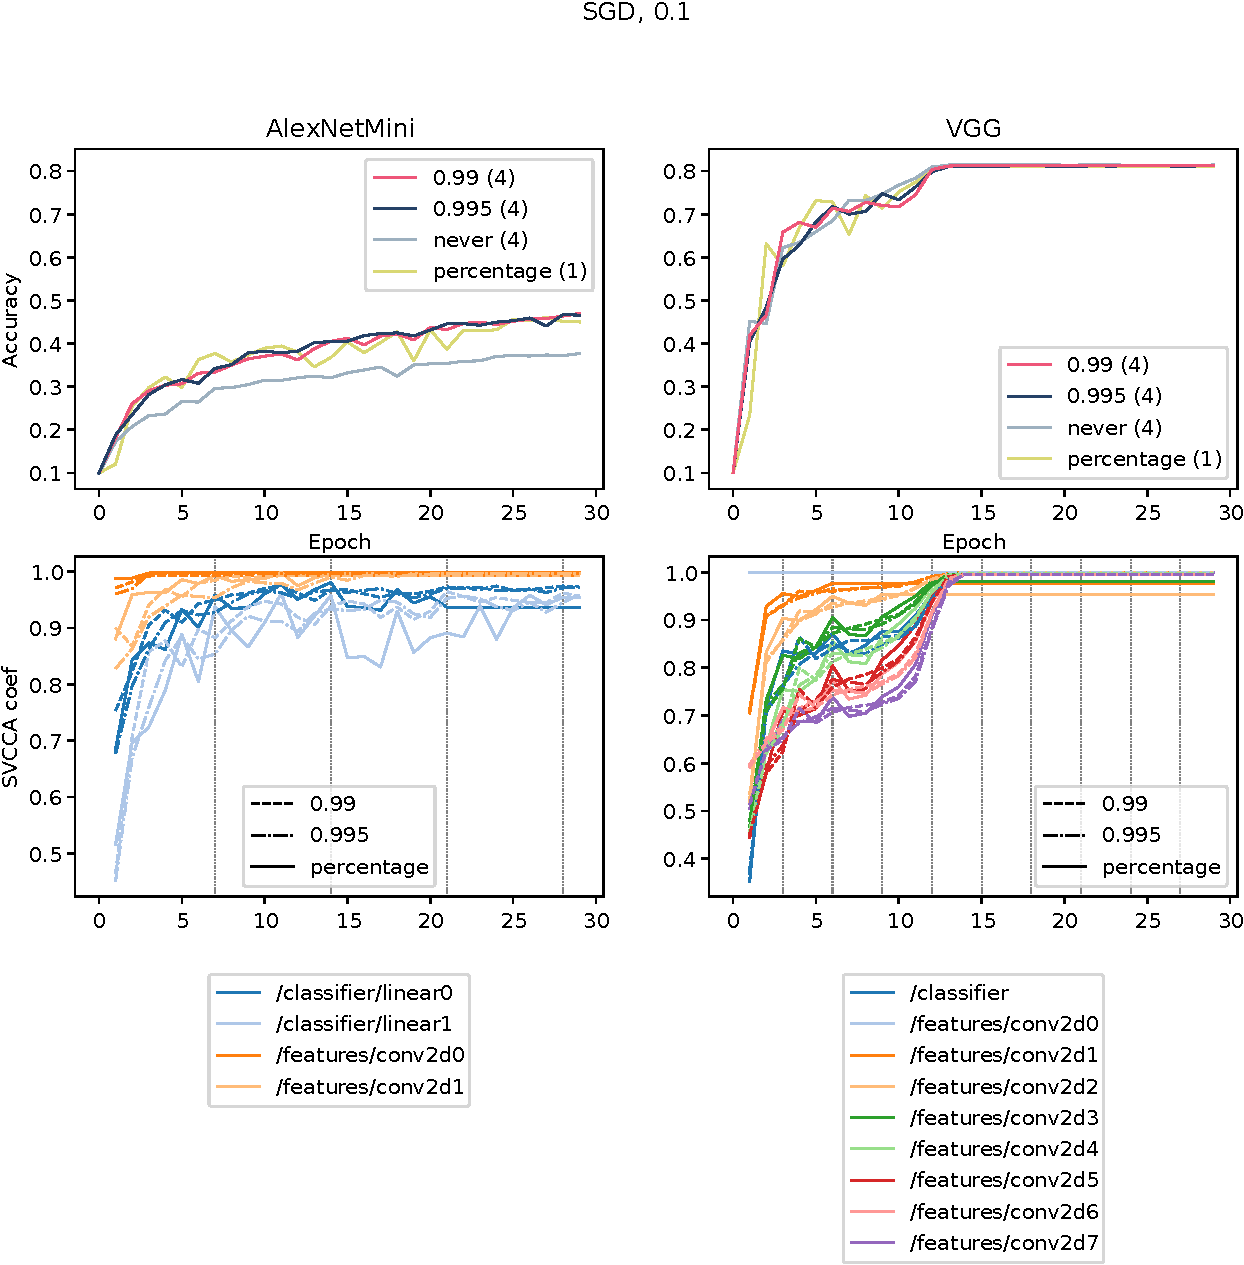
\includegraphics[width=\linewidth]{gfx/diagrams/experiments/saturation/acc_sim_alexnetmini_vgg_sgd_01.pdf}
        \caption{Accuracy and self-similarity for learning rate $0.1$}
        \label{fig:saturation_alexnet_vgg_sgd_001_similarity}
    \end{subfigure}

    \begin{subfigure}{\textwidth}
        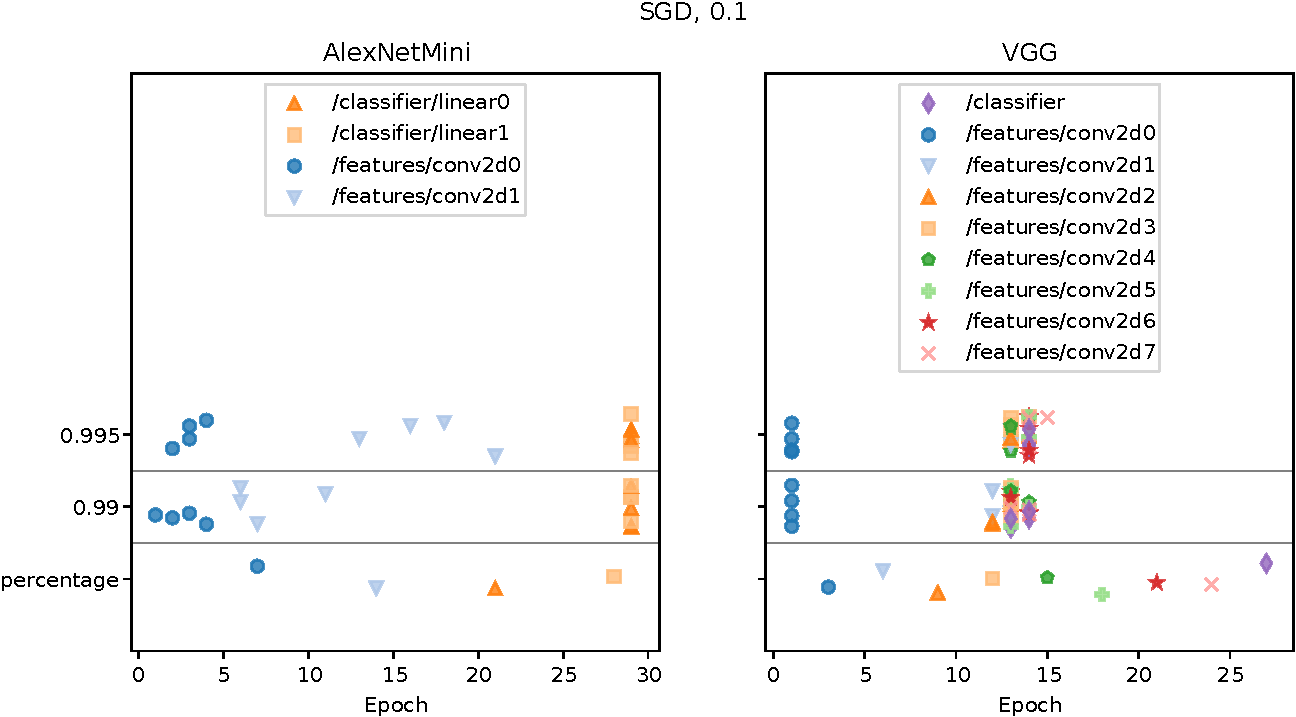
\includegraphics[width=\linewidth]{gfx/diagrams/experiments/saturation/convergence_alexnetmini_vgg_sgd_01.pdf}
        \caption{Freeze points for learning rate $0.1$}
        \label{fig:saturation_alexnet_vgg_sgd_01_convergence}
    \end{subfigure}
\end{figure}

\begin{figure}
    \centering
    \caption{Layer convergence experiment with learning rate $0.5$}
    \label{fig:saturation_alexnet_vgg_sgd_05}
    \begin{subfigure}{\textwidth}
        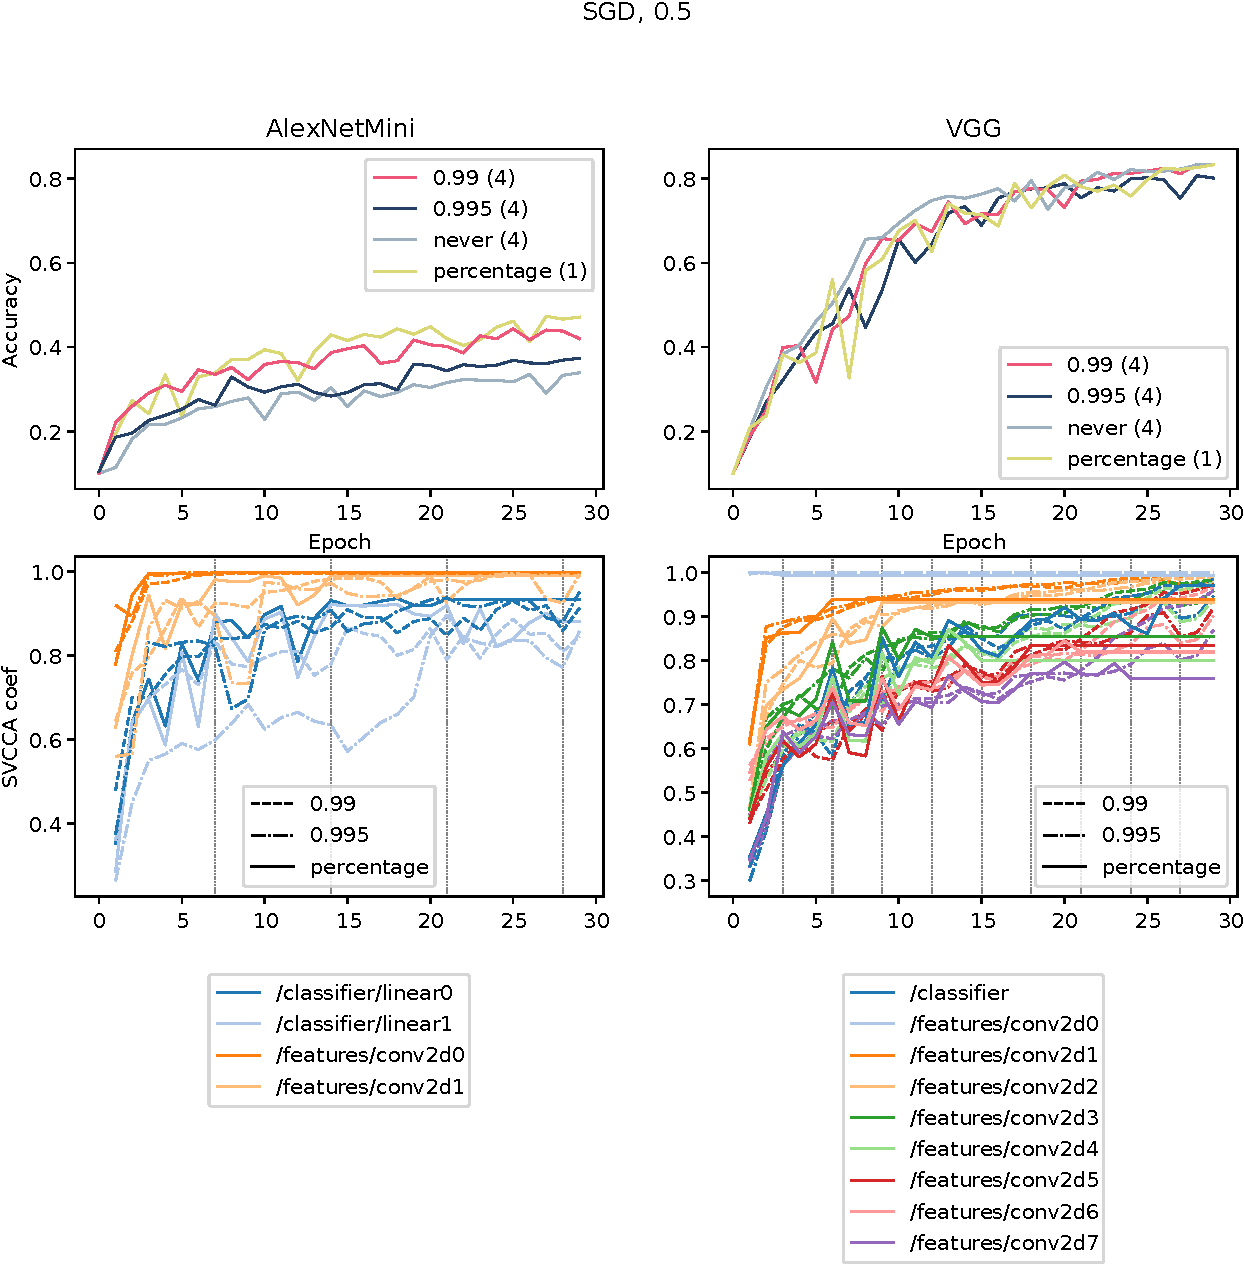
\includegraphics[width=\linewidth]{gfx/diagrams/experiments/saturation/acc_sim_alexnetmini_vgg_sgd_05.pdf}
        \caption{Accuracy and self-similarity for learning rate $0.5$}
        \label{fig:saturation_alexnet_vgg_sgd_05_similarity}
    \end{subfigure}

    \begin{subfigure}{\textwidth}
        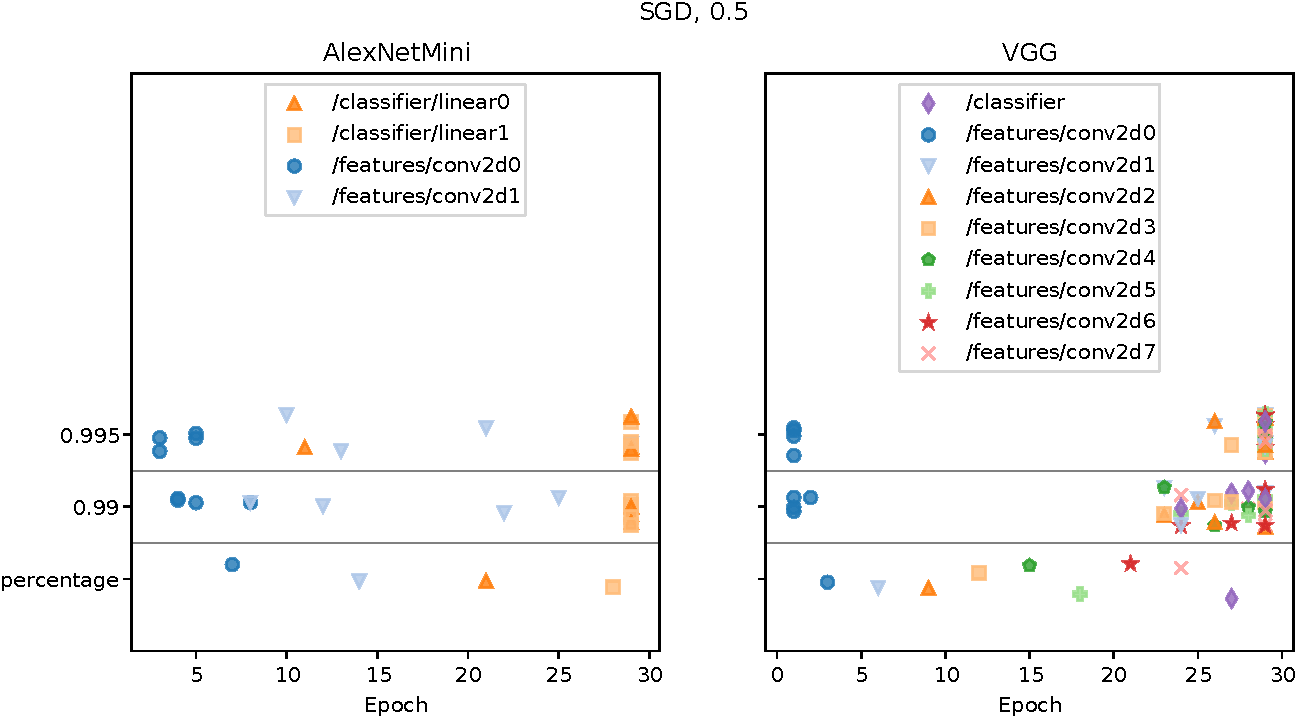
\includegraphics[width=\linewidth]{gfx/diagrams/experiments/saturation/convergence_alexnetmini_vgg_sgd_05.pdf}
        \caption{Freeze points for learning rate $0.5$}
        \label{fig:saturation_alexnet_vgg_sgd_05_convergence}
    \end{subfigure}
\end{figure}

As a last point, the high learning rate used in
\cref{fig:saturation_alexnet_vgg_sgd_05_similarity} leads to interesting reactions in the
self-similarity metric. While AlexNetMini's performance is not much worse than
for the optimal learning rate of $0.1$, training is much more unstable, with the
accuracy fluctuating. Indeed, the saturation metric reflects this constant
change in layer weights, and most of the layers do not converge at all. This
observation opens the door for evaluating the SVCCA score as a stability metric
and for guiding learning rate scheduling (see
\cref{sec:detecting_learning_rate_problems}). Both AlexNetMini and VGG exhibit
much slower convergence than would be possible, and we can read the instability
from the SVCCA score's trajectory.

\subsubsection{Computational Savings with Self-Similarity vs. Fixed Schedule}

Turning to the question of whether this heuristic performs better than the fixed
schedule from \citep{raghu2017svcca}, the point at which each layer was frozen
is graphed in
\cref{fig:saturation_alexnet_vgg_sgd_001_convergence,fig:saturation_alexnet_vgg_sgd_01_convergence,fig:saturation_alexnet_vgg_sgd_05_convergence}.
Layers are differentiated by colour and marker style, and all runs are
displayed. A random offset is added in the vertical direction to avoid the runs
overlapping.

In most cases, using self-similarity---without negatively impacting accuracy --
tends to freeze layers earlier, thus saving more computation than freezing
layers at fixed percentages of training time.
\cref{fig:saturation_alexnet_vgg_sgd_001_convergence} (both models) and
\cref{fig:saturation_alexnet_vgg_sgd_01_convergence} (VGG model) both show the
similarity-based freezing to freeze layers much earlier on average. As the high
learning rate of $0.5$ leads to unstable training, with likely very high
variance in the weight updates, it is unsurprising that layers don't converge
and are thus trained until the end. For non-pathological cases, the proposes
metric appears to save more update steps. However, additional overhead is
incurred in actually computing the metrics. An exhaustive evaluation of the
cost-benefit tradeoff is left for future work, but the results are promising,
especially in light of a possible GPU implementation of SVCCA, most of which
could be done asynchronously.

For the smaller of the two models (left plots), we see again that the two
convolutional layers areconverged right after the first epoch or the second,
respectively. The precise threshold value does not seem to matter so much.
Saturating the first linear layer takes much longer and the different thresholds
lead to different times until convergence. A higher learning rate of $0.1$ (see
\cref{fig:saturation_alexnet_vgg_sgd_01_convergence}) leads to more spaced-out
convergence points for the convolutional layers, while the linear layers are not
considered converged during training at all. What can be deduced from this fact
is that the $0.01$ is a too small learning rate for the problem and architecture
in question. The reason why the linear layers converge early for a learning rate
of $0.01$ could be that the learning rate is simply too small to translate the
gradients on this problem into substantial change in the layer's weights,
leading to a smaller validation accuracy. By contrast, the larger learning rate
will move the weights sufficiently to allow the linear layers to learn more
performant representations, and thus need longer to converge. Similar
observations can be made for a learning rate of $0.5$.

In case of the VGG model, we observe similarly fast convergence of the first
convolutional layers, reinforcing the hypothesis that the early feature
detectors are mostly architecture- and problem-agnostic. We can also see that
convergence for most layers takes longer for higher thresholds (unsurprisingly),
except for the medium learning rate
(\cref{fig:saturation_alexnet_vgg_sgd_01_convergence}) for which all layers very
consistently converge at the same time as well. Since this is the condition with
the best validation accuracy, this phenomenon may merit further investigation.

For the high learning rate of $0.5$, most VGG layers do not converge at all
according to the self-similarity metric. Nevertheless, the accuracy does reach
optimal levels $\sim 0.8$, but takes much longer than with a smaller learning
rate. This tells us that whether or not all layers converge is not necessarily
indicative of whether the network can learn the task at all, but more likely how
quickly and efficiently it can learn it. An investigation into how the solutions
found by networks with converged layers differ from unconverged ones is an
interesting application for the SVCCA metric as well. As a matter of fact,
\citet{NIPS2018_7815} use it to compare minimisers found by memorising and
generalising networks.


\subsection{Summary}%
\label{sub:svcca-conclusion}

This section has demonstrated an alternative use case for the SVCCA similarity
metric originally proposed for offline-introspection of neural networks. It was
evaluated as a heuristic for detecting layer convergence which resulted in
promising observations when compared to freezing layers at a fixed schedule. The
SVCCA self-similarity does not usually deteriorate performance and freezes
layers earlier than a fixed schedule in many cases.
More comprehensive studies should be made to validate this observation on more
architectures and datasets. Furthermore, the role of the additional parameters
introduced for computing the SVCCA metric remains to be explored---notably, how
many datapoints should be used. As computing the metric in a certain interval
incurs some computation overhead which we have not yet accounted for, more work
is necessary to definitivly answer the question whether this heuristic
outperforms the fixed schedule in absolute terms, not only in number of gradient
computations saved.
